\documentclass[hyperref={bookmarks=false},aspectratio=169]{beamer}
\usepackage[utf8]{inputenc}
%\usepackage[latin1]{inputenc}
\usepackage{amsmath}
\usepackage{xmpmulti}
\usepackage{amssymb}
\usepackage{mathrsfs}
\usepackage{animate}
\usepackage{lmodern}
\usepackage{multirow,rotating}
\usepackage{color}
\usepackage{xcolor}
\usepackage{hyperref}
\usepackage{tikz-cd}
\usepackage{array}
\usepackage{mathtools,nccmath}%
\usepackage{etoolbox, xparse} 
\usepackage[all]{xy}
\usepackage{xmpmulti}
\usepackage{comment}

\definecolor{greenn}{RGB}{34 139 34}
%\usepackage{transparent}
%\setbeamertemplate{section in toc shaded}[default][50]
%\setbeamertemplate{subsection in toc shaded}[default][50]

%\usepackage{enumitem}
%\usepackage{etoolbox}
\usetikzlibrary{matrix,decorations.pathreplacing}
 %\usepackage[frenchb]{babel}
\def\singR{\mathcal{X}_{R}}
\def\singRbar{\mathcal{\overline{X}}_{R}}

\newcommand*{\graybullet}{\textcolor{gray}{\textbullet}}
\newcommand*{\bluebullet}{\textcolor{blue}{\textbullet}}
\newcommand*{\redbullet}{\textcolor{red}{\textbullet}}

\hypersetup{bookmarks=true,unicode=true,pdftoolbar=true,pdfmenubar=true,
	pdffitwindow=false,pdfstartview={FitH},pdftitle={UMSSM},
	pdfauthor={O. Ozdal}, pdfsubject={CAP2017},
	pdfcreator={O. Ozdal},pdfproducer={O. Ozdal}, pdfkeywords={Non-minimal 
		supersymmetry}{Beyond the Standard Model Physics}{sneutrino dark matter},
	pdfnewwindow=true,colorlinks=true,
	linkcolor=,citecolor=magenta,filecolor=magenta,urlcolor=cyan}



\NewDocumentCommand{\tens}{t_}
{%
	\IfBooleanTF{#1}
	{\tensop}
	{\otimes}%
}
\NewDocumentCommand{\tensop}{m}
{%
	\mathbin{\mathop{\otimes}\displaylimits_{#1}}%
}

% ---------------  Define theme and color scheme  -----------------
\usetheme[sidebarleft]{Caltech}  % 3 options: minimal, sidebarleft, sidebarright

%\setbeamertemplate{footline}[frame number]

% ------------  Information on the title page  --------------------
\title[]
{\bfseries{Gestion synchronisée de la production d'hydrogène et des tournées de véhicules autonomes (SMEPC)}}% (Hydrogen)
%Gestion synchronisée de la production d'hydrogène et de sa consommation par des véhicules autonomes
%\subtitle{Problem description}

\author[]
{{%\textit{Présenté par}  
Eloise Yollande MOL\'{E} KAMGA}  %\textit{($3^{e}$ année de doctorat)}
\vspace{0.1cm} 
	\\ {\textit{Sup.} Fatiha Bendali \and Jean Mailfert \and  Alain Quilliot  \and  Hélène Toussaint  }}
\institute[Clermont Auvergne University]
{
      
	 Soutenance de thèse de Doctorat \\ LIMOS - CNRS, Université Clermont Auvergne
}

\date{18 Juillet 2023}%16 Juin 2021
\titlegraphic{
\includegraphics[width=1.8cm]{./figures/logo_limos_coul_def.png}
\hspace{1.5cm}  
\includegraphics[width=2.5cm]{./figures/imob.jpg}
\hspace{1.5cm}  
\includegraphics[width=2cm]{./figures/region.jpg}
\hspace{1.5cm}  
\includegraphics[width=0.8cm]{./figures/Logo-UCA.png}}

%------------------------------------------------------------

%------------------------------------------------------------
%The next block of commands puts the table of contents at the 
%beginning of each section and highlights the current section:

\AtBeginSection[]
{
%\setbeamertemplate{page number in head/foot}{}
 \addtocounter{framenumber}{-1}
  \begin{frame}
    \frametitle{Plan}
    %\addtocontents{toc}{\protect\thispagestyle{empty}}
    \tableofcontents[currentsection]
  \end{frame}
 % \setbeamertemplate{page number in head/foot}[frame number]
}


%------------------------------------------------------------
%\addtobeamertemplate{footline}{\insertframenumber/\inserttotalframenumber}

%\setbeamertemplate{page number in head/foot}[framenumber]

\setbeamertemplate{footline}[frame number]

\usepackage{csquotes}
%\newcommand{\guillemets}[1]{« #1 »}
\begin{document}

\frame{\titlepage}  % Creates title page


%---------   table of contents after title page  ------------
\begin{frame}
\frametitle{Plan}
\transboxout
\tableofcontents
\end{frame}
%---------------------------------------------------------

\section{Introduction}
\begin{frame}
\frametitle{Contexte et objectif}
\begin{itemize}
\item \textbf{Contexte local} : PAVIN (Plateforme Auvergnate pour Véhicules intelligents) plateforme dédiée aux expérimentations scientifiques sur des véhicules.% intelligents.% (planification de tournées, production d'énergies renouvelables : hydrogène produite par photolyse, etc.).
\pause
\item \textbf{Contexte sociétal} :
\begin{itemize}
\item Montée en Force des Energies Renouvelables : Hydrogène Solaire, Photo-
Voltaïque, BioMasse, etc.
\item Emergence de plate-formes de production In Situ : Problématique de l’Auto-Consommation.
%\item L'autoconsommation induit un haut niveau de synchronisation
\end{itemize}

%\item Apparition de producteurs locaux d'énergies : mettre en place un SGPPLE (Système de Gestion d'une Plateforme de Production Locale d'\'{E}nergie)
%\item  \textcolor{red}{Véhicules hybrides} : \textbf{cette nouvelle génération de véhicules apportent de nouvelles contraintes}.



\end{itemize}

	\begin{columns}[t]
\column{.3\textwidth}
\centering

\includegraphics[width=2.5cm]{./figures/imobs3.jpg}
\column{.3\textwidth}
\centering
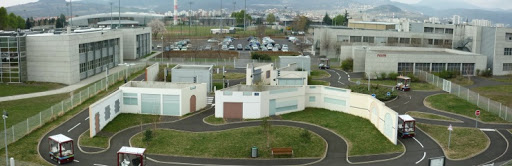
\includegraphics[width=5cm]{./figures/pavinn.jpg}%PAVIN.png
%\footnote{http://www.inmc21.com/}
\column{.3\textwidth}
\centering

\includegraphics[width=2cm]{./figures/Investissements_d'avenir_-_logo.jpeg}
\end{columns}

%\pause
 \begin{alertblock}{Notre objectif}
 %Concevoir des algorithmes pour planifier de façon \textbf{synchrone} la production d'hydrogène par photolyse et les tournées des véhicules. 
 Concevoir des modèles et algorithmes propres à permettre la synchronisation entre une
production locale d’Hydrogène Solaire et sa consommation par une flotte de véhicules
autonomes.

 \end{alertblock}
\end{frame}

\begin{frame}
\frametitle{Revue de la littérature (1/2)}
\centering{
\begin{tabular}{|c|c|c|c|c|} 
\hline
 Références & Recharge & Product. & Synchro. & \# recharges \\ \hline
 %Problème & oui & oui  & oui  & MIP & 1\\ \hline % one hydrogen vehicle, one recharging station 
\cite{article_Conrad} & \checkmark & \times  & \times& plusieurs \\ \hline %many electrics 
%vehicles,many recharging stations 
%[\textcolor{blue}{1}]
\cite{Erdeli}  & \checkmark & \times &\times  &plusieurs \\ \hline 
%[\textcolor{blue}{2}]
 \cite{Shrouf} &  \times & \checkmark &\times &  \times \\ \hline 
 %[\textcolor{blue}{3}]
 \cite{Grimes} & \times & \checkmark & \times& \times \\ \hline %\cite{Joon-Yung}\\ 
 \cite{Michael} & \times & \times& \checkmark& \times%\cite{Joon-Yung}
 %[\textcolor{blue}{4}]
 \\\hline
\end{tabular}
}
\vspace{0.01}
{\footnotesize 
\begin{thebibliography}{5}
%\setlength{\itemsep}{0.5pt}
%\setlist[thebibliography]{itemsep=5pt}
\begin{enumerate}
 \bibitem[1]{article_Conrad}
    Ryan Conrad et al. %, Miguel Figliozzi.
	\textcolor{black}{The Recharging Vehicle Routing Problem.}
	Proc. of the 61st Annual IIE Conference, 2011.
 \bibitem[2]{Erdeli}
    Tomislav Erdelić et al. %, Tonci Caric, Martina  Ravlic, Leo Tišljarić.
	\textcolor{black}{Electric vehicle routing problem with single or multiple recharges.}
	Transportation Research Procedia, 2019.%40: 217-224,
 \bibitem[3]{Shrouf}
    Fadi Shrouf et al. %, Joaquín Ordieres-Meré, García-Sánchez, Álvaro Miguel Ortega-Mier.
	\textcolor{black}{Optimizing the production scheduling of a single machine to minimize total energy consumption costs.}
	Journal of Cleaner Production, 2014.%67:0 197–207,
\bibitem[4]{Grimes}
    Helio Yochihiro et al. %, Jinwoo Park.
	\textcolor{black}{A survey of case studies in production scheduling: Analysis and perspectives}
	Journal of Computational Science, 2018.% 52:13 3922-3939, 
 %\bibitem[4]{Grimes}
 %   Joon-Yung Moon et al.%, Jinwoo Park.
%	\textcolor{black}{Smart production scheduling with time-dependent and machine-dependent electricity cost by considering distributed energy resources and energy storage.}
%	International Journal of Production Research, 2014.% 52:13 3922-3939, 
\bibitem[5]{Michael}
    Michael Drexl. 
    \textcolor{black}{Synchronization in Vehicle Routing, A Survey of VRPs with Multiple Synchronization Constraints.}
   Transportation Science, 2012.%46(3):297–316,
\end{enumerate}
\end{thebibliography}
}

%\begin{tabular}{c|c|c|c|c} 
% & Recharge & Product.  & Méthodes & \# recharges \\ \hline%& Synchro. 
 %Problème & oui & oui  & oui  & MIP & 1\\ \hline % one hydrogen vehicle, one recharging station 
%\cite{article_Conrad} & \checkmark & \times  & Construction itérative & plusieurs \\ \hline %many electrics 
%vehicles,many recharging stations 
%[\textcolor{blue}{1}]
%\cite{Erdeli}  & \checkmark & \times   & Ruin-recreate/MIP &plusieurs \\ \hline 
%[\textcolor{blue}{2}]
 %\cite{Shrouf} &  \times & \checkmark  & Algo. génétique &  \times \\ %\hline 
 %[\textcolor{blue}{3}]
 %\cite{Grimes} & \times & \checkmark & PPC/MIP & \times \\ \hline %\cite{Joon-Yung}\\ 
 %\cite{Grimes} & \times & \checkmark & PPC/MIP & \times%\cite{Joon-Yung}
 %[\textcolor{blue}{4}]
%\end{tabular}
%Ruin-recreate : similaire au recuit simulé (on doit juste faire de grande modication de la solution)

%Recuit simulé : À chaque itération de l'algorithme une modification élémentaire de l'état est effectuée. Cette modification entraîne une variation {\displaystyle \Delta _{E}}\Delta _{E} de l'énergie du système (toujours calculée à partir du critère que l'on cherche à optimiser). Si cette variation est négative (c'est-à-dire qu'elle fait baisser l'énergie du système), elle est appliquée à l'état courant. Sinon, elle est acceptée avec une probabilité {\displaystyle e^{-{\frac {\Delta _{E}}{T}}}}e^{{-{\frac  {\Delta _{E}}{T}}}}. Ce choix de l'exponentielle pour la probabilité s'appelle règle de Metropolis.

%PPC : La programmation par contraintes (PPC, ou CP pour constraint programming en anglais) est un paradigme de programmation apparu dans les années 1970 et 19801,2 permettant de résoudre des problèmes combinatoires de grande taille tels que les problèmes de planification et d'ordonnancement3. En programmation par contraintes, on sépare la partie modélisation à l'aide de problèmes de satisfaction de contraintes (ou CSP pour Constraint Satisfaction Problem), de la partie résolution dont la particularité réside dans l'utilisation active des contraintes du problème pour réduire la taille de l'espace des solutions à parcourir (on parle de propagation de contraintes).

%Algo. génétiques: Les algorithmes génétiques utilisent la notion de sélection naturelle et l'appliquent à une population de solutions potentielles au problème donné. La solution est approchée par « bonds » successifs, comme dans une procédure de séparation et évaluation (branch & bound), à ceci près que ce sont des formules qui sont recherchées et non plus directement des valeurs.On itère ensuite selon ce procédé en gardant la température constante.
%\hspace{2cm}
%\scriptsize{
%\begin{itemize}
%\item [1] Ryan Conrad, Miguel Figliozzi. {\emph{The Recharging Vehicle Routing Problem}.}{\emph{Proc. of the 61st Annual IIE Conference}, 2011.}
%Cette recherche présente le problème de l'itinéraire des véhicules de recharge (RVRP), une nouvelle variante du problème bien connu de l'itinéraire des véhicules (VRP) où les véhicules à autonomie limitée sont autorisés à se recharger chez les clients en cours de route. Le problème a des applications pratiques potentielles dans les problèmes d'acheminement du monde réel où des véhicules électriques avec des capacités de recharge rapide peuvent être utilisés pour des livraisons de moins d'un camion (LTL) dans les zones urbaines. Le problème général est présenté comme un problème capacitif (CRVRP) et un problème capacitif avec contraintes de fenêtre temporelle du client (CRVRP-TW). Un énoncé du problème est formulé et les résultats expérimentaux ainsi que les limites de solution dérivées sont présentés. Des résultats intuitifs sont observés lorsque l'autonomie du véhicule est limitée et lorsque le temps de recharge est long. Il est également démontré que la longueur moyenne de la tournée est fortement corrélée avec les limites de la solution dérivée. Les estimations de la longueur moyenne de la tournée peuvent être utilisées dans une application de planification pour estimer les coûts et la consommation d'énergie en fonction des caractéristiques du véhicule et du client.


%\item [2] Tomislav Erdelić, Tonci Caric, Martina  Ravlic, Leo Tišljarić. \emph{Electric vehicle routing problem with single or multiple recharges.} \emph{Transportation Research Procedia, 40: 217-224, 2019.}
%Aujourd'hui, en raison des nouvelles lois et politiques relatives aux émissions de gaz à effet de serre et de la prise de conscience sociale et écologique croissante de la durabilité des transports, les entreprises de logistique ont commencé à intégrer les technologies vertes dans leurs activités de distribution. Ici, les véhicules électriques, en tant que mode de transport plus propre que les véhicules conventionnels, occupent le devant de la scène et de nombreuses entreprises intègrent déjà des véhicules électriques dans leur flotte de livraison. Par rapport aux véhicules conventionnels, les véhicules électriques ont une autonomie plus courte en raison de la capacité limitée de la batterie, et ils doivent être rechargés plus fréquemment dans des stations de recharge. Pour gérer efficacement la flotte de véhicules électriques, de nouveaux algorithmes qui prennent en compte les visites aux stations de recharge doivent être développés. Dans cet article, nous avons observé le problème de routage des véhicules électriques avec les fenêtres de temps (E-VRPTW) et les politiques de recharge multiple ou unique pendant le trajet. Le parc homogène de véhicules électriques à batterie avec une charge et une capacité de batterie limitées, les fenêtres temporelles des clients et la recharge linéaire complète aux stations de recharge sont pris en compte. L'objectif est de minimiser la distance totale parcourue tout en utilisant un nombre minimal de véhicules. Pour trouver la solution au problème, nous avons appliqué, dans les grandes instances, la métaheuristique basée sur le principe de la ruine-récréation -----(ruin-recreate principle)---- et, dans les petites instances, nous avons résolu le programme de nombres entiers mixtes avec un logiciel commercial.

%\item [3] Fadi Shrouf, Joaquín Ordieres-Meré, García-Sánchez, Álvaro Miguel Ortega-Mier.\emph{Optimizing the production scheduling of a single machine to minimize total energy consumption costs.} \emph{Journal of Cleaner Production, 67: 197–207, 2014.}
%La hausse du coût de l'énergie est l'un des facteurs importants associés à l'augmentation des coûts de production dans les usines de fabrication, ce qui encourage les décideurs à aborder ce problème de différentes manières. Une étape importante dans cette tendance est la réduction des coûts de consommation d'énergie des systèmes de production. En tenant compte des prix variables de l'énergie pendant une journée, ce document propose un modèle mathématique pour minimiser les coûts de consommation d'énergie pour la programmation de la production d'une seule machine pendant les processus de production. En prenant des décisions au niveau de la machine pour déterminer les temps de lancement du traitement des tâches, les temps d'inactivité, le moment où la machine doit être arrêtée, le temps de "mise en marche" et le temps d'"arrêt", ce modèle permet au responsable des opérations de mettre en œuvre la planification de la production la moins coûteuse pendant un quart de travail. Pour obtenir des solutions "presque" optimales, la technologie des -----algorithmes génétiques----- a été utilisée. En outre, pour déterminer si la solution heuristique offre le coût minimum et le meilleur calendrier possible pour minimiser les coûts énergétiques, une solution analytique a également été mise en œuvre pour générer la solution optimale. Ensuite, une comparaison entre la solution analytique et les solutions heuristiques est présentée ; pour les problèmes plus importants, la solution heuristique est préférable. Les résultats indiquent que des réductions significatives des coûts énergétiques peuvent être obtenues en évitant les périodes de prix élevés de l'énergie. Ce processus de minimisation a également un effet positif sur l'environnement en réduisant la consommation d'énergie pendant les périodes de pointe, ce qui augmente la possibilité de réduire les émissions de CO2 des sites de production d'électricité.
%\item [4]	Joon-Yung Moon, Jinwoo Park.\emph{Smart production scheduling with time-dependent and machine-dependent electricity cost by considering distributed energy resources and energy storage.} \emph{International Journal of Production Research, 52:13 3922-3939, 2014.}
%De nombreux pays tentent activement de faire face aux effets récents du changement climatique et de la crise énergétique. Dans le même temps, l'utilisation efficace de l'énergie et la réduction des émissions de gaz à effet de serre sont très importantes, non seulement pour réduire les coûts énergétiques, mais aussi pour contribuer à un mode de vie durable et respectueux de l'environnement. Actuellement, dans certains pays, les industries manufacturières paient des tarifs d'électricité stratifiés qui dépendent de l'heure de la journée (c'est-à-dire la charge de pointe, la charge moyenne et la charge hors pointe). Par conséquent, le processus de programmation de la production, qui tient compte des coûts de l'électricité en fonction du temps et des machines, permet à ces industries de minimiser les dépenses énergétiques. En outre, le réseau intelligent émergent est censé exiger des industries qu'elles paient les coûts horaires de l'électricité en temps réel. Une planification de la production plus efficace et plus intelligente sur le plan énergétique est donc un objectif majeur. Ce document traite de la minimisation du coût total de production du problème de la planification flexible des ateliers. Notre méthode permet à chaque décideur de l'industrie manufacturière de chercher une solution de compromis pour les coûts totaux de production, en considérant les coûts de l'électricité avec les ressources énergétiques distribuées et le stockage de l'énergie. Nous utilisons des approches de programmation par contraintes et de programmation mixte pour résoudre ce problème, et nous comparons les modèles que nous proposons avec la méthode de calcul classique.

%\item [5]	Craig Grimes, Oomman Varghese, Sudhir Ranjan. \emph{Light, water, hydrogen: The solar generation of hydrogen by water photoelectrolysis.  Springer-Verlag US, 2008.}
%\end{itemize}


%}
%\pause\vspace{2}


\end{frame}


\begin{frame}
\frametitle{Revue de la littérature (2/2)}
\begin{itemize}
\item Planification des tournées de véhicules et leur alimentation en energie
\end{itemize}
\begin{figure}
	\centering
    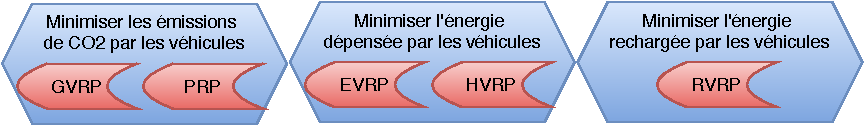
\includegraphics[width=\textwidth]{./figures/Etat_art_recharge.pdf}
	%\caption[Problèmes incluant tournée de véhicules et gestion de leurs alimentations]{Classes de problèmes qui incluent tournée de véhicules et gestion de leurs alimentations.}
	\label{Etat_art_recharge}
\end{figure}

%Canhong Lin, K.L. Choy, G.T.s Ho, Sai-Ho Chung, and H. Lam. Survey of green vehicle routing
%problem : Past and future trends. Expert Systems with Applications, 41 :1118–1138, 03 2014.

\begin{thebibliography}{2}
%\setlength{\itemsep}{0.5pt}
%\setlist[thebibliography]{itemsep=5pt}
%\begin{enumerate}
 
  \bibitem[1]{article_Conrad}
    Canhong Lin et al. %, Miguel Figliozzi.
	\textcolor{black}{Survey of green vehicle routing problem : Past and future trends.}
	Expert Systems with Applications, 2014.
 
 \bibitem[2]{article_Erdelić}
    Tomislav Erdelić et al. %, Miguel Figliozzi.
	\textcolor{black}{A Survey on the Electric Vehicle Routing Problem: Variants and Solution Approaches.}
	Journal of Advanced Transportation, 2019.
%\end{enumerate}
\end{thebibliography}
\end{frame}

\section{Problématique}

\subsection{SMEPC : formulation générale} 



%\begin{frame} : 
%\frametitle{SMEPC à Tour Fixé}
%\end{frame}

\begin{frame}
\frametitle{Formulation générale SMEPC : véhicules et stations (1/3)}

%\begin{altenv}<7>{texte avant}{texte apres}
%{autre texte avant}{autre texte apres}
%\end{altenv}

\begin{minipage}{.4\textwidth}%
 \begin{center}
\begin{figure}
    \centering%\textwidth
    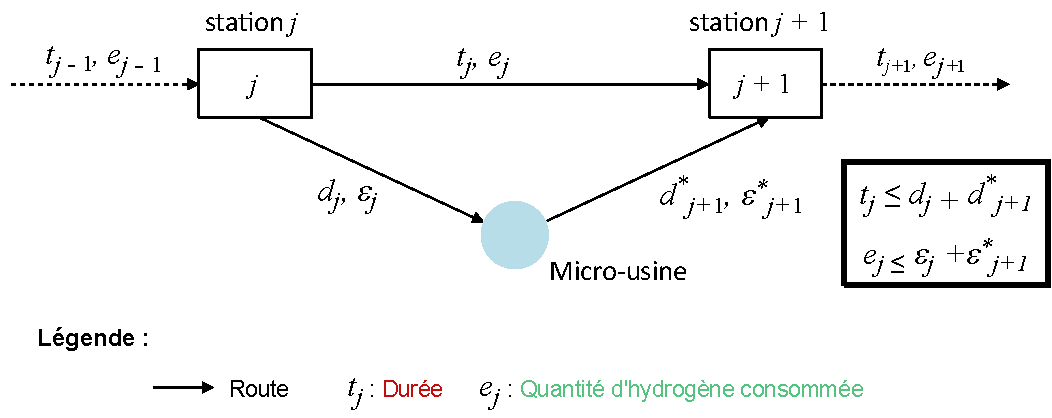
\includegraphics[width=11cm]{./figures/slide_Fr_Notation_inputs.pdf}%load_french(2)(1).pdf
    
    \label{fig:my_label}
\end{figure}
\end{center}
\end{minipage}%
\hfill
\vspace{3}
\begin{minipage}{.9\textwidth}%
\begin{itemize}
    \item Plusieurs véhicules alimentés en hydrogène et ayant chacun un réservoir limité.
    \space
    \item Chaque véhicule :
    \begin{itemize}
      \item départ et retour dépôt.
     \space
    \item  doit parcourir les stations dans un ordre à déterminer.%effectuer des \textcolor{blue}{requêtes} (transports d'objets) 
    \space
    \item  utilise du \textcolor{red}{temps} et de l'\textcolor{greenn}{énergie} pour réaliser cela.
     \space
    \item  a un temps maximal donné pour effectuer sa tournée.
    \space
    \item peut aller à la micro-usine se recharger en cours de tournée.
    
    \end{itemize}
    
\end{itemize}
\end{minipage}%

\end{frame}


%\begin{frame}
%\multiinclude[format=pdf]{./figures/tourn}
%\end{frame}

\begin{frame}
\frametitle{Formulation générale SMEPC : dépôt et micro-usine (2/3)}
%\begin{itemize}
%\item We have a depot which produces hydrogen and contains electric terminals.
%\item All vehicles can come to charge energy in the depot.
%\end{itemize}



\begin{minipage}{.50\textwidth}%
\begin{figure}
    \centering
    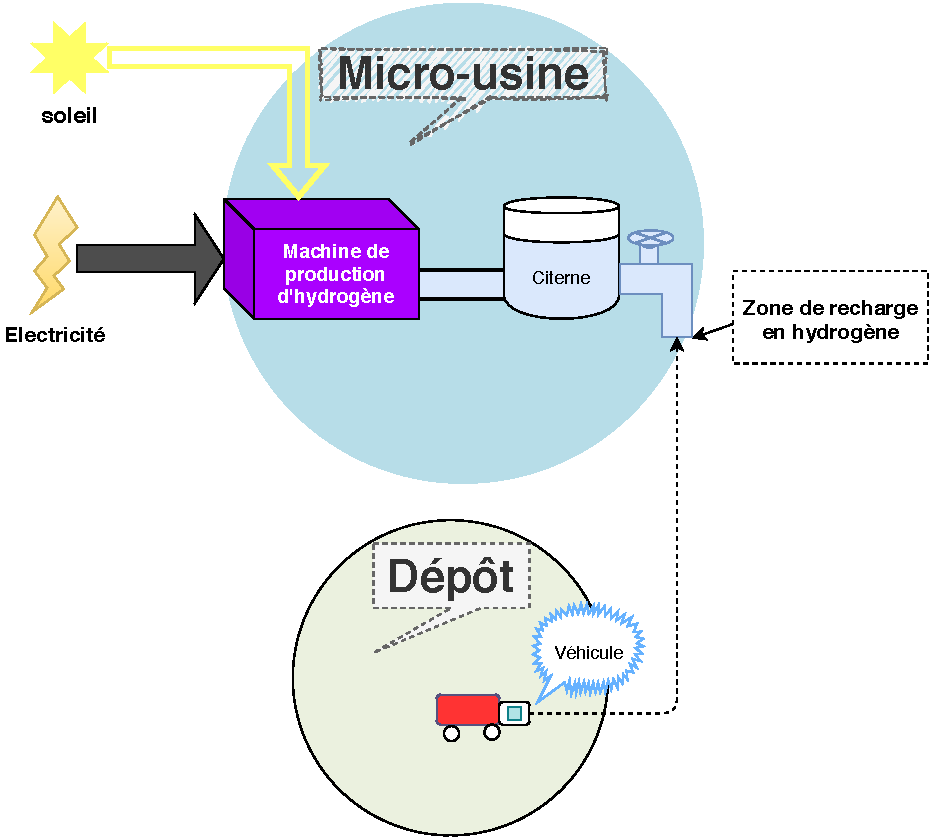
\includegraphics[width=\textwidth]{./figures/illustration_depotrond.pdf}%depotfinal_french(1)(3)
   % \caption{Illustration du \textcolor{gray}{dépôt} et de la \textcolor{blue}{micro-usine} de production d'hydrogène.}
    \label{fig:dept}
\end{figure}

\end{minipage}%
\hfill
\begin{minipage}{.5\textwidth}%
%\textbf{Contraintes} :
\begin{itemize}
 
    \item L'hydrogène est produite par photolyse dans une micro-usine.
    \space
    \item Les rendements et coûts de production dépendent de l'ensoleillement.
    \space
    \item \`{A} la fin de la tournée, le réservoir et la citerne doivent être au moins aussi remplis qu'au départ.
\end{itemize}   
 \setbeamercolor{itemize item}{fg=red}
%\textbf{Hypothèses} :
%%\begin{itemize}
    
%%    \space
%%    \item \`{A} la fin de la tournée, le réservoir et la citerne doivent être au moins aussi remplis qu'au départ.
%%\end{itemize}
\end{minipage}%
%	\centering
%	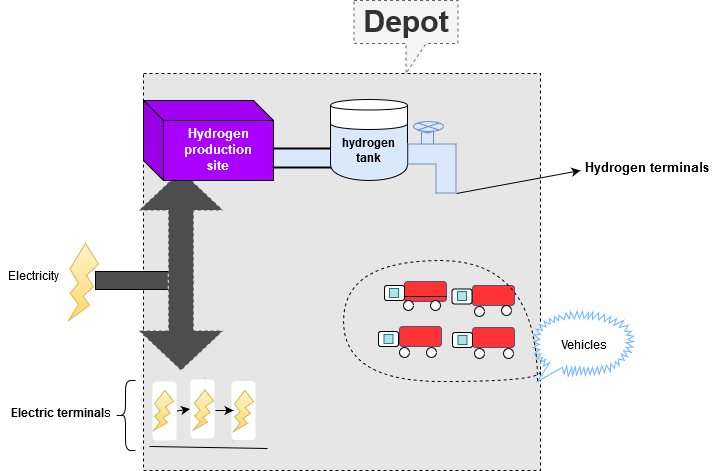
\includegraphics[scale=0.45]{./figures/depotfinal(2)-ENGLISH.png}


\end{frame}

\begin{frame}
\frametitle{Formulation générale SMEPC : but et difficultés (3/3) } 

%\begin{itemize}
%\item Difficultés :
%\begin{itemize}

%\item Gestion algorithmique du comportement autonome des véhicules ;
%\item Gestion algorithmique du mécanisme de synchronisation ;
%\item Gestion algorithmique de la dimension collaborative dans les procédés ;% (Comportement autonome des véhicules)
%\item Aspect collaboratif : synchronisation des recharges des véhicules et de la production d’hydrogène;
%\item  %(prévisions météorologiques).
%   \end{itemize}    
%\end{itemize} 

\begin{block}<+->{Objectifs}
\begin{itemize}
 \item Planifier le parcours de chaque véhicule en incluant les recharges de façon à optimiser la qualité du
tour du point de vue du \textit{Vehicle Manager}.
  \item Planifier de façon synchrone la production d’hydrogène de façon à minimiser les coûts de
production du point de vue du \textit{Production Manager}.
 \end{itemize}
 \end{block}
 \begin{alertblock}<+->{Principales difficultés}
\begin{itemize}
 
 \item Interaction entre les deux décideurs (convergence des agendas, %compromis
 schéma bi-objectif, %simultané
 bi-niveau,%maitre esclave
 etc.).
 \item Synchronisation entre processus production et véhicules.
  \item Incertitude sur la production.
  \item Autonomie des véhicules (gestion des risques et de la sécurité, optimisation dynamique des tournées, etc.).
\end{itemize}
 \end{alertblock}
\end{frame}

\subsection{SMEPC à Tour Fixé}%pb avec hypothèses simplificatrices
\begin{frame}
\frametitle{Plan}
\addtocounter{framenumber}{-1}
\tableofcontents[currentsection,currentsubsection]
\end{frame}

\begin{frame}
\frametitle{SMEPC à Tour Fixé : hypothèses simplificatrices (1/2)}

\begin{block}{Hypothèses}
\begin{itemize}
\item Un seul véhicule.
\item La tournée est fixée.
\item Combiner les critères associés au véhicule et à la production en un
seul critère.
\item Contexte déterministe.
\item Production et recharge ne se font pas simultanément.
 \end{itemize}
 \end{block}
\end{frame}

\begin{frame}
\frametitle{SMEPC à Tour Fixé : exemple de solution (2/2)}
%\begin{itemize}
%\item We have a depot which produces hydrogen and contains electric terminals.
%\item All vehicles can come to charge energy in the depot.
%\end{itemize}



\begin{minipage}{.75\textwidth}%
\begin{figure}
    \centering
    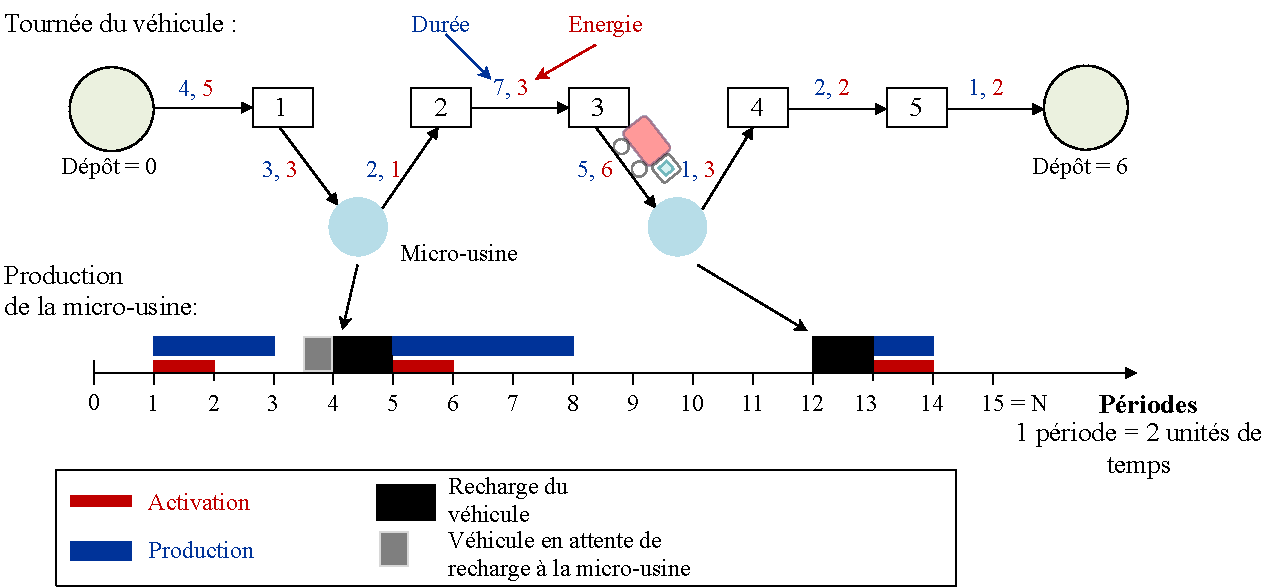
\includegraphics[width=\textwidth]{./figures/Synchro_exemple.pdf}%Dessin62.pdf
    \caption{Synchronisation de la tournée (véhicule) et de la production d'hydrogène (micro-usine).}
    \label{fig:dept}
\end{figure}
\end{minipage}%
\hfill
\pause
\begin{minipage}{.25\textwidth}%
    \begin{enumerate}
 \item  Planifier les recharges en hydrogène du \textcolor{red}{véhicule} en :
 \begin{itemize}
 \item  Minimisant la durée de la tournée.
 \end{itemize}
 \item Planifier la \textcolor{blue}{production} d'hydrogène en :
 \begin{itemize}
 \item   Minimisant le coût de production.
 \end{itemize}

 \end{enumerate}

\end{minipage}%
%	\centering
%	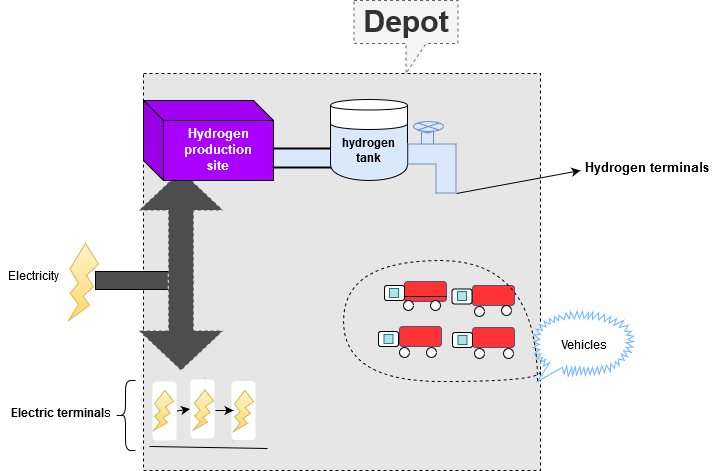
\includegraphics[scale=0.45]{./figures/depotfinal(2)-ENGLISH.png}


\end{frame}

%\begin{frame}
%\frametitle{Le problème : exemple de solution (3/3)}

%\begin{alertblock}{Buts}
 %\begin{enumerate}
 %\item  Planifier les recharges en hydrogène du véhicule en :
% \begin{itemize}
 %\item  Minimisant la durée de la tournée.
% \end{itemize}
 %\item Planifier la production d'hydrogène en :
 %\begin{itemize}
% \item   Minimisant le coût de production.
% \end{itemize}

% \end{enumerate}
% \end{alertblock}
%\hspace{0.2}
%\begin{figure}
 %   \centering
%    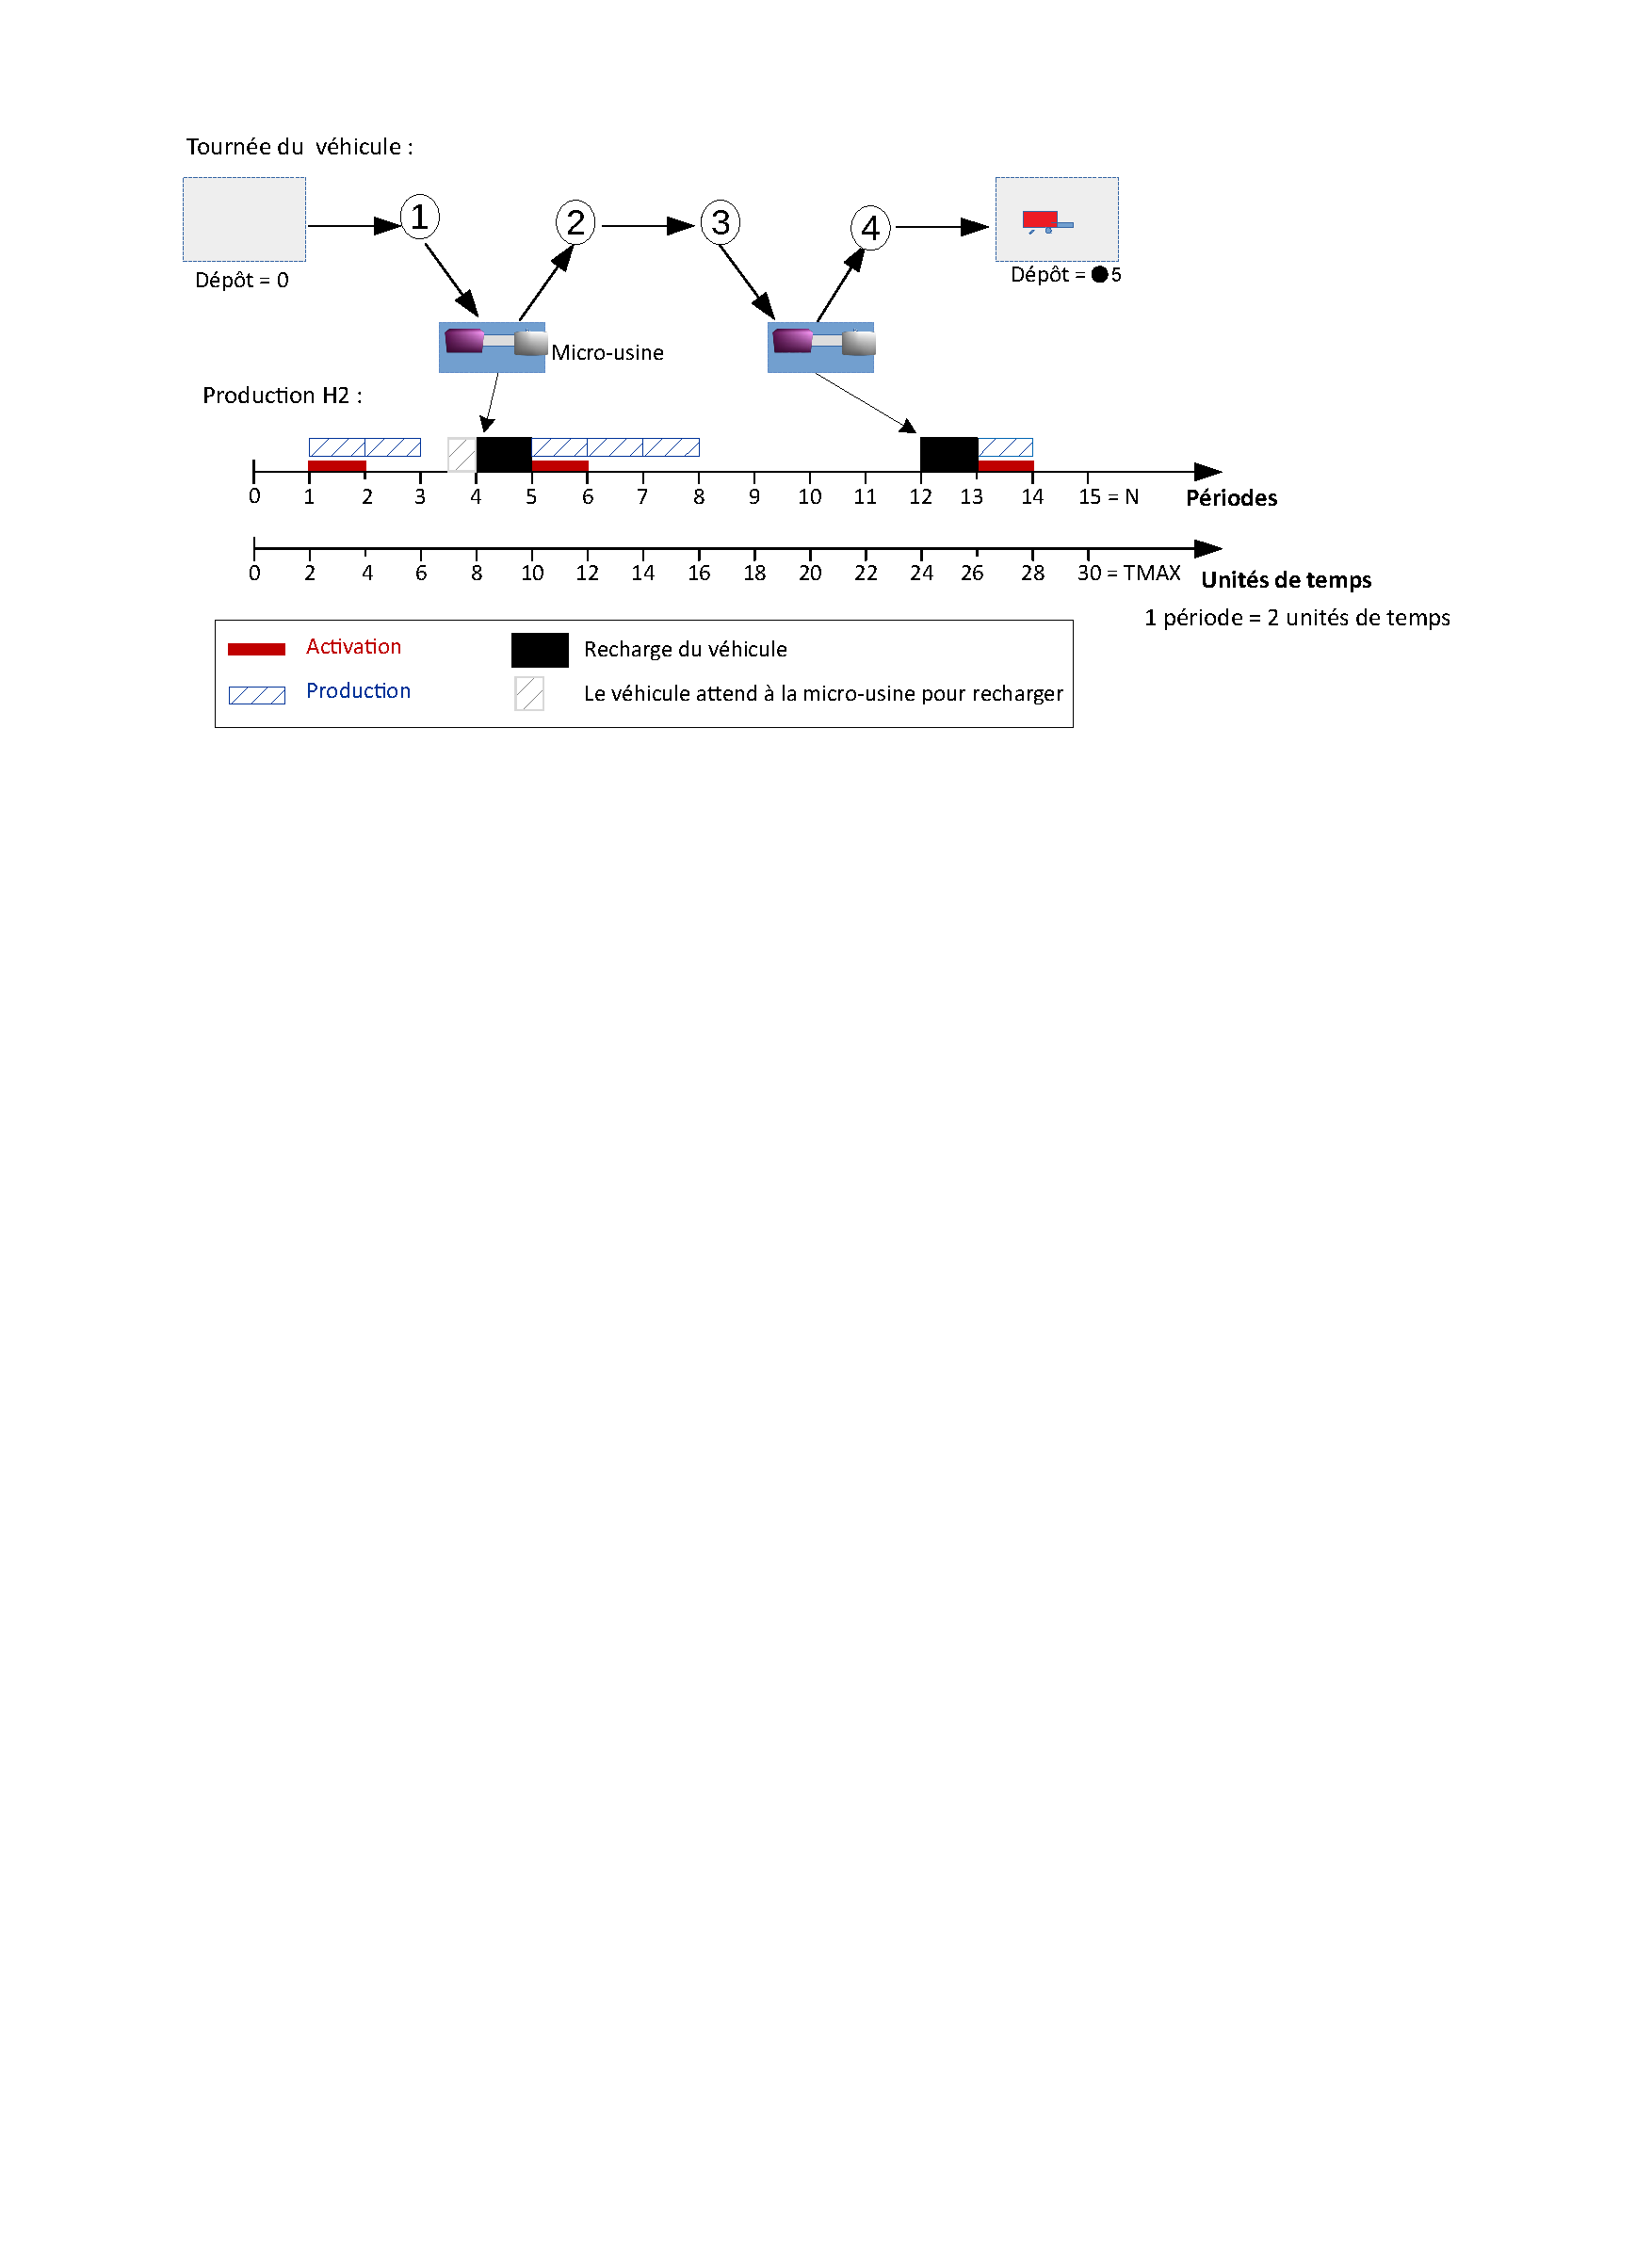
\includegraphics[width=9cm]{./figures/Dessin62.pdf}
 %   \caption{Exemple de solution du problème.}
 %   \label{fig:my_label}
%\end{figure}
%\end{frame}



%\section{Revue de la littérature}


\begin{frame}
\frametitle{Décomposition du problème}
%\begin{itemize}
%\item This system contains two subsystems : recharging system and production system.
%\end{itemize}

%\begin{minipage}{.80\textwidth}%
\begin{center}
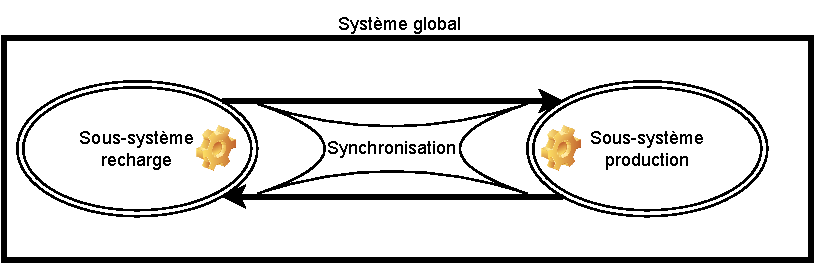
\includegraphics[width=\textwidth]{./figures/slide_synchronisation_pb.pdf}
\end{center}
%\end{minipage}%
%\hfill
%\begin{minipage}{.4\textwidth}%
\begin{itemize}
\item Découpage du problème en deux sous-problèmes :
\begin{enumerate}
 \item  problème du véhicule ;
 \item  problème de production.
  %\item  \textit{Durée de la recharge fixée}
 \end{enumerate}
 \end{itemize}
%\end{minipage}%

\end{frame}








%--------------------------------------------------------



%--------------------------------------------------------


%--------------------------------------------------------

 
%--------------------------------------------------------


%---------------------------------------------------------

%\subsection{Problème du véhicule}



%\end{frame}
\begin{frame}

\frametitle{problème du véhicule : RVRP (1/2)}
%\begin{itemize}

%\item We have many stations which are connected by roads.
%\item We know for each road its duration and energies requirements. %(hydrogen and electricity).
%\item Each station has a request : picking up or delivering packages.
%\item Stations, vehicule, dépôt.
%\end{itemize}
\begin{itemize}

		\begin{block}{Hypothèse}%<+->{Hypothèse}
		\begin{itemize}
		 % \item Ordre de visite des stations fixé.
 \item  On a une quantité infinie d'hydrogène dans la citerne à la micro-usine.

		\end{itemize}


 \end{block}
 \pause
   \space 
    \begin{alertblock}{Objectifs}%<+->{Objectifs}
    Planifier les recharges du véhicule en minimisant un critère qui combine : 
\begin{enumerate}
 \item La durée de la tournée.
  \item L'énergie consommée par le véhicule.
 \end{enumerate}
 \end{alertblock}
  
\pause

\end{itemize}
\begin{figure}
    \centering
    \tiny{durée de la tournée = $4+3+\textcolor{blue}{duree\_rech}+2+7+5+\textcolor{blue}{duree\_rech}+1+2+1=25+2\times \textcolor{blue}{duree\_rech}$ }
    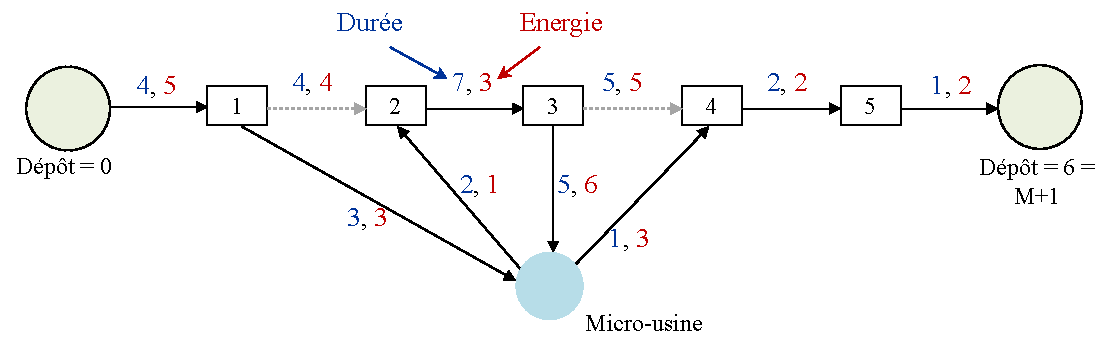
\includegraphics[width=12cm]{./figures/Trip.pdf}
    %\caption{Une tournée de véhicule avec deux opérations de recharge avec $TMax=30$.}
    \label{fig:dept}
\end{figure}

\end{frame}

%\begin{frame}
%\frametitle{Complexité de RVRP}

 %\end{frame}
%\begin{frame}

%\frametitle{Description recharging problem}

	%\centering
  	%\centering
	%\cenering
 		%wentering
 		%\centeng
	%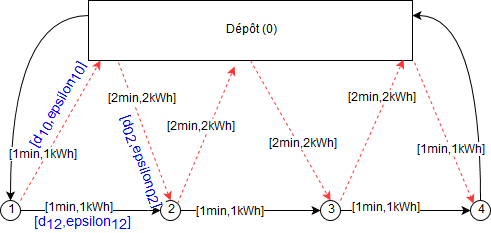
\includegraphics[scale=0.480]{./figures/recharg.png}



%\end{frame}


%\begin{itemize}
%\item We have a depot which produces hydrogen and contains electric terminals.
%\item All vehicles can come to charge energy in the depot.
%\end{itemize}


%%\begin{frame}
%%\frametitle{Exemple de tournée (2/2)}
%%\begin{minipage}{.75\textwidth}%
%%\begin{figure}
%%    \centering
%%    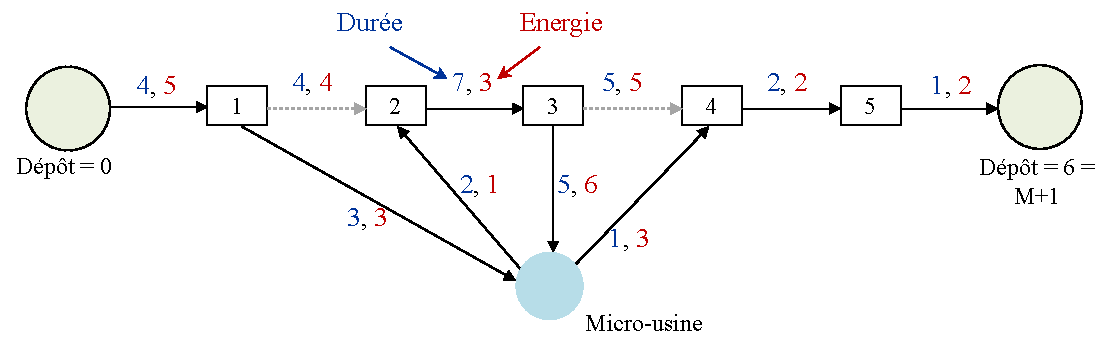
\includegraphics[width=\textwidth]{./figures/Trip.pdf}
 %%   \caption{Une tournée de véhicule avec deux opérations de recharge avec $TMax=30$.}
 %%   \label{fig:dept}
%%\end{figure}
%%\end{minipage}%
%%\hfill
%%\begin{minipage}{.25\textwidth}%
 %%   \frametitle{Exemple de tournée (2/2)}

%%\begin{itemize}
%%    \item Hydrogène initiale du véhicule : $E_0= 8$ ;
%%    \item Capacité du réservoir : $C^{Veh}=15$ ;
%%    \item \textbf{Solution} : une tournée est  0-1-MU-2-3-MU-4-5-0.
%%\end{itemize}

%%\end{minipage}%
%%\end{frame}
%	\centering
%	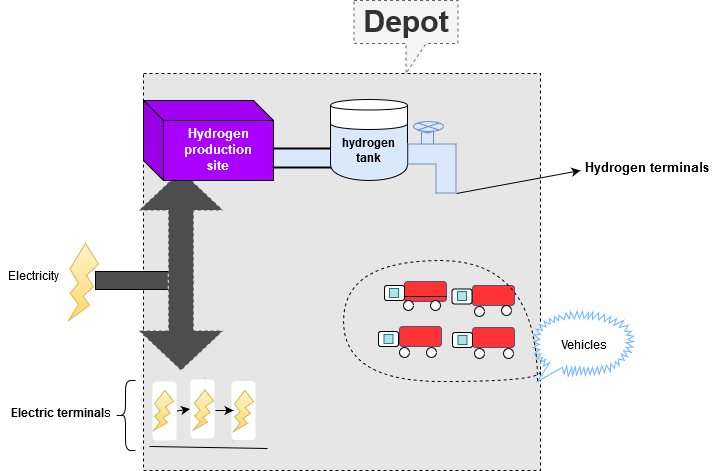
\includegraphics[scale=0.45]{./figures/depotfinal(2)-ENGLISH.png}



%	\begin{columns}[t]
%\column{.5\textwidth}

%\begin{figure}
 %   \centering
    %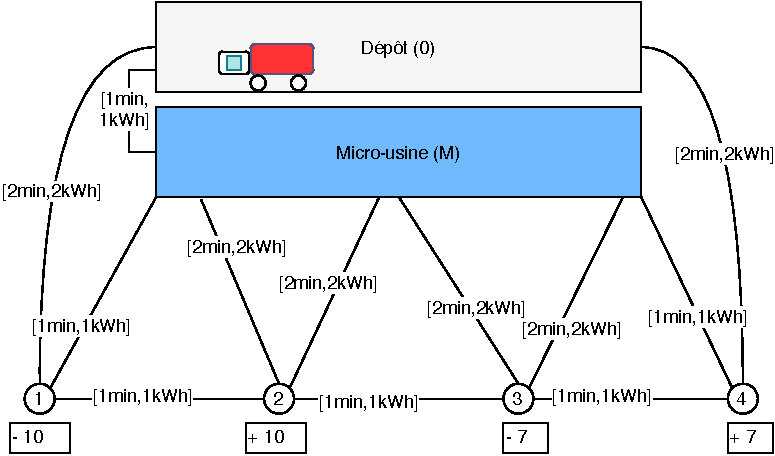
\includegraphics[width=5.3cm]{./figures/new recharg_french_ar(2)(1).pdf}
    %\caption{Une instance du problème du véhicule.}
    %\label{fig:my_label}
%\end{figure}

%\column{.5\textwidth}
%\begin{figure}
%    \centering
    %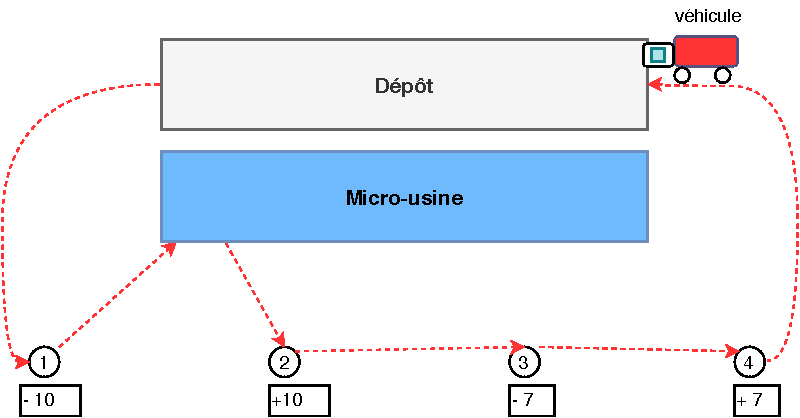
\includegraphics[width=6cm]{./figures/tousr_french(3).pdf}
    %\caption{Une solution du problème du véhicule.}
    %\label{fig:my_label}
%\end{figure}


%\end{columns}

%\begin{frame}
%\transduration<0-1>{0}
%            \multiinclude[<+->][format=pdf, graphics={width=\textwidth}]{./figures/tourn}
%\end{frame}
%\begin{frame}

%\frametitle{Complexity}

	%\centering
  	%\centering
	%\cenering
 		%wentering
 		%\centeng
	%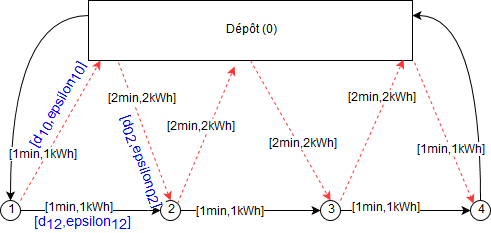
\includegraphics[scale=0.480]{./figures/recharg.png}



%\end{frame}




%\subsection{Problème de production}


\begin{frame}
\frametitle{Problème de production}% (1/2)
	\begin{itemize}
	   
	   % \item La micro-usine peut être démarrée (coût fixe) et arrêtée. 
	    %\item The start-up cost is given, but we don't have a stop cost.
	    
	\end{itemize}
		\begin{block}<+->{Hypothèse}
		\begin{itemize}
 \item On connait toutes les demandes du véhicule. 
 %\item Chaque demande doit être satisfaite.
 \end{itemize}
\end{block}
 %\centering
%	
\includegraphics[scale=0.21]{./figures/stop.jpg}
	\begin{alertblock}<+->{Objectifs}
	Déterminer la stratégie de production de l'hydrogène : %dont le véhicule aura besoin en :
\begin{enumerate}
 
 \item Minimisant les coûts de production.
 \item Satisfaisant les recharges le plus rapidement possible.
 \end{enumerate}
 \end{alertblock}
%\end{frame}

%\begin{frame}
%\frametitle{Description production problem}
	


 %
	   


	
%\end{frame}

%\begin{frame}
%\frametitle{Description production problem}


	

%\end{frame}
%---------------------------------------------------------

%\begin{frame}
%\frametitle{Exemple de stratégie de production (2/2)}
	\begin{columns}[t]
	\column{.5\textwidth}
	\only<3->{\begin{figure}
    \centering
    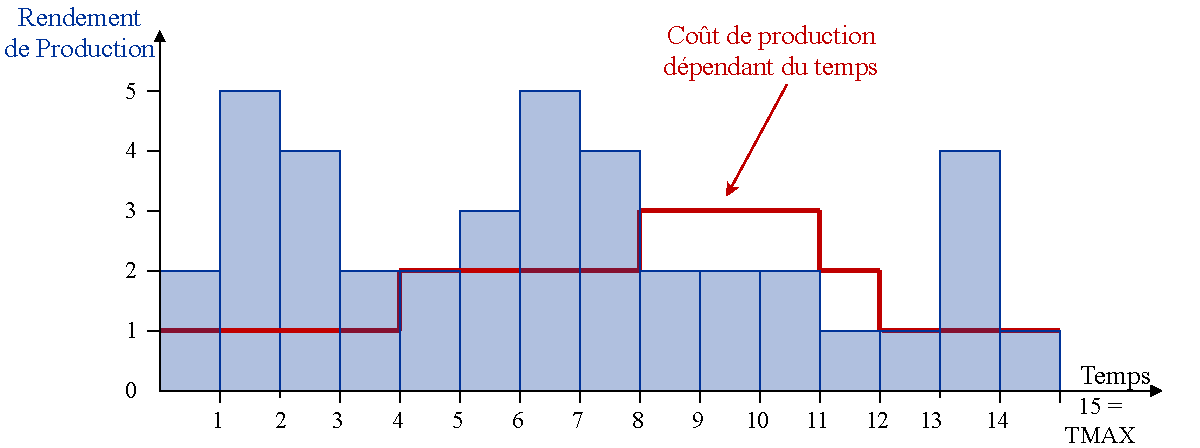
\includegraphics[width=6cm]{./figures/Dessin3.pdf}
   % \caption{Une instance du problème de production avec $H_0=4$, $Cost^F=7$, $C^{Tank}=15$.}
    \label{fig:my_label}
\end{figure}}

\column{.5\textwidth}
\only<4->{\begin{figure}
    \centering
      \tiny{coût de production = $\textcolor{red}{7\times3} +1+1+2+2+2+1=30$ }
    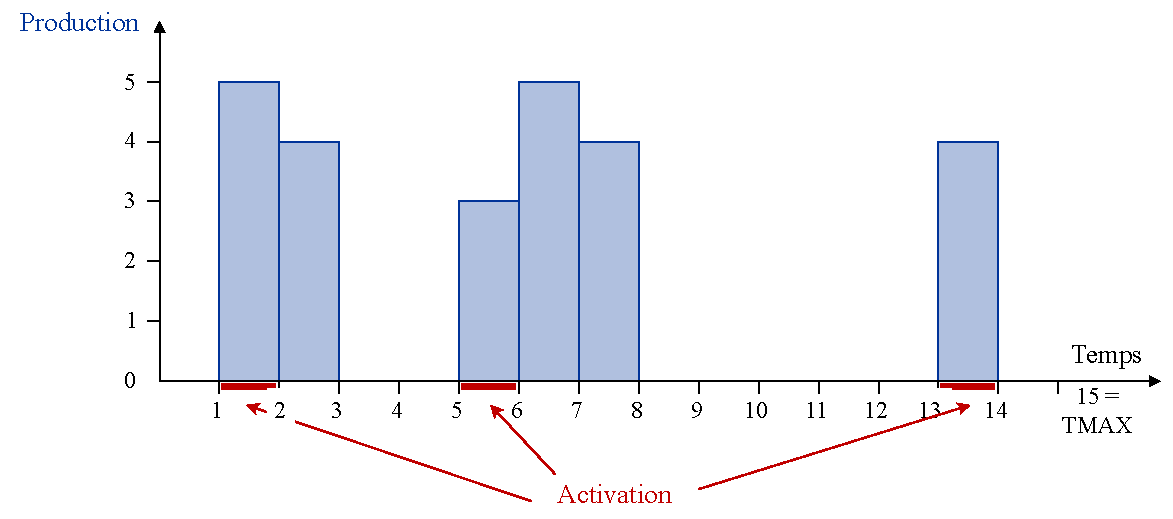
\includegraphics[width=5.5cm]{./figures/Dessin2(1).pdf}
    %\caption{Une solution du problème de production.}
    \label{fig:my_label}
     
\end{figure}}
	\end{columns}
\end{frame}
% $H_0=4$, $TMax=30$, $Cost^F=7$, $C^{Tank}=15$, $C^{Veh}=15$


%--------------------------------------------------------

%---------------------------------------------------------




\section{Résolution exacte à Tour Fixé}
\subsection{Modèle \textbf{\textit{MILP}}}%\textbf{\textit{LR}} : Relaxation %Programmation linéaire à variables mixtes}
\begin{frame}
\frametitle{Modèle : données, variables et fonction objectif (1/3)}
\begin{minipage}{.45\textwidth}%

\textbf{Données} :
\begin{enumerate}
	\item Véhicule : \textcolor{red}{$M$}, $C^{Veh}$, $E_0$ ;
		%\begin{itemize}
		%\item \textcolor{blue}{$M$}, $C^{Veh}$, $E_0$ ;
   %\item \forall j=0, ..., M, $t_j$, $d_j$, $d_j^*$, $e_j$, $\varepsilon_j$, $\varepsilon_j^*$.% $\Gamma$,
		%\end{itemize}
	\item Production
		\begin{itemize}
		  \item $N$, $C^{Tank}$, $H_{0}$, \textcolor{blue}{$Cost^F$} ; 
            \item $\textcolor{blue}{Cost_i^V}, \forall i=0, ..., N-1$ .%, $R_i$, $P_i=[p\times i, p\times(i+1)[$.
		\end{itemize}
	\item Paramètre : $\alpha$
		%\begin{itemize}
		%  \item $\alpha$
		%\end{itemize}
\end{enumerate}
\pause
\textbf{Variables} :
\begin{enumerate}
	\item Véhicule
	   \begin{itemize}
		      \item $x_j$, $L_j$, $\forall j=0, ..., M$;
        
        \item  $T_j^*$, $V^{Veh}_j$, $\textcolor{red}{T_j}$,   $\forall j=0, ..., M+1$. 
	   \end{itemize}
		
	\item Production
		\begin{itemize}
				\item $\textcolor{blue}{z_i}$, $\textcolor{blue}{y_i}$, $\delta_i$, $\forall i=0, ..., N-1$ ;
    
    \item  $V_i^{Tank}$, $\forall i=0, ..., N$.%$L^*_i$	;%
	  \end{itemize}
	\item Synchronisation
		\begin{itemize}
			\item \textcolor{greenn}{$U_{i,j}$ \forall i=0, ..., N-1, \forall j=0, ..., M}
	  \end{itemize}
	%\item Linéarisation
	%\begin{itemize}
	%\item  \forall i=0, ..., N-1, \forall j=0, ..., M, $m_{i,j}$
	%\end{itemize}
\end{enumerate}

\end{minipage}%
\pause
\hfill
\begin{minipage}{.55\textwidth}%
\textbf{Mon objectif} :
\begin{equation*}
\label{d13}
%\boxed{
\textbf{Min}	\sum_{i=0}^{N-1}[(\textcolor{blue}{Cost^F} \times \textcolor{blue}{y_i}) + (\textcolor{blue}{Cost_i^V} \times \textcolor{blue}{z_i})]+ \alpha \times \textcolor{red}{T_{M+1}}
%}
\boxe
\end{equation*}
\end{minipage}%

\end{frame}	
	
\begin{frame}	
\frametitle{Modèle : contraintes véhicule et producion (2/3)}
\begin{enumerate}
%\item Fonction objectif
%\begin{equation}
%\label{d13}
%%\boxed{
%\textbf{Min}	\sum_{i=0}^{N-1}[(\textcolor{red}{Cost^F} \times \textcolor{red}{y_i}) + (\textcolor{red}{Cost_i^V} \times \textcolor{red}{z_i})]+ \alpha \times \textcolor{blue}{T_{M+1}}
%%}
%	\boxe
%\end{equation}
%\item Contraintes :
%\begin{itemize}
%\item Contraintes sur le véhicule 
%%\begin{itemize}
%%\item évolution du stock d'hydrogène du véhicule ;
%%\item évolution des dates d'arrivées aux stations ;
%%\item calcul des quantités rechargées.
%%\end{itemize}
%\item Contraintes sur la production d'hydrogène
%%\begin{itemize}
%%\item calcul des dates de démarrage et arrêt de la micro-usine ;
%%\item évolution du stock d'hydrogène de la citerne.
%%%\item calcul des dates du stock
%%\end{itemize}
%\item Contraintes de synchronisation
%\begin{itemize}
%\item Dates recharge ;
%\item Dates usine.
%%\item calcul des dates du stock
%\end{itemize}
%\end{itemize}

%\end{frame}

%\begin{frame}
	
%\frametitle{Modèle : contraintes véhicule et production (3/4)}
\item \textbf{\textcolor{red}{Contraintes véhicule}} 
\begin{itemize}

\small{
\item Evolution du \textbf{stock d'hydrogène} du \textbf{véhicule} ;
% Véhicule :
%\begin{center}
	\begin{equation}
	%\boxed{% \left\{
		\begin{array}{lll}
			% &V_0^{Veh} = E_0, V_{M+1}^{Veh} \geq E_0& \squad \\
	        %&V_j^{Veh} \leq C^{Veh}& \squad $\forall j = 1 \dots M+1$\\
			%&V_j^{Veh} \geq \varepsilon_j & \squad $\forall j = 0 \dots M$\\
			&V_{j+1}^{Veh} = V_j^{Veh}-e_j + x_j \times(e_j-\varepsilon_j-\varepsilon_{j+1}^*) +L_j & \squad $\forall j = 0 \dots M$\\
			
	\end{array}
		%\right.
	%}
	\end{equation}
%\end{center}
}

\item Evolution des \textbf{dates d'arrivées} aux stations ;

\small{
%\begin{center}
	\begin{equation}
	%\boxed{% \left\{
		\begin{array}{lll}
			%&T_0=0, T_{M+1} \leq TMax & \squad \\
			&T_{j+1} \geq (1-x_j)\times (T_j+t_j)+x_j \times (T_j^*+p +d_{j+1}^*)  & \squad    \forall j = 0 \dots M\\
			%&T^*_j \geq T_j +d_j & \squad $\forall j = 0 \dots M$\\
		
	\end{array}
		%\right.
	%}
	\end{equation}
%\end{center}
}

%\item Calcul des quantités rechargées.

%\small{
%\begin{center}
%	\begin{equation}
%	%\boxed{% \left\{
%		\begin{array}{lll}
			%&L_j \geq 0, L_j \leq C^{Veh}&  $\forall j = 0 \dots M$\\
			%&L_j \leq C^{Veh} \times x_j& \squad $\forall j = 0 \dots M$\\
%			&C^{Veh} + \varepsilon_j - V_j^{Veh} \leq L_j \leq C^{Veh} & \squad $\forall j = 0 \dots M$\\
%	\end{array}
		%\right.
%	%}
%	\end{equation}
%\end{center}
%}

\end{itemize}
\pause
\item \textbf{\textcolor{blue}{Contraintes production}} 
\begin{itemize}
%\small{
%\item Production et recharge ne se réalisent jamais simultanément ;

%%Production :
%%\begin{center}
%	\begin{equation}
%	%\boxed{%Production \left\{
%		\begin{array}{lll}
			%&z_0 = y_0&\\
%			 &z_i+\delta_i \leq 1 &\quad $\forall i = 0 \dots N-1$ \\
            %&y_i=1 \rightarrow (z_{i-1}=0 \land z_i=1)& \quad $\forall i = 1 \dots N-1$\\
			
	
%		\end{array}
		%\right.
	%}
%	\end{equation}
%\end{center}
%}
\item Evolution du \textbf{stock d'hydrogène} de la \textbf{citerne} ;

\small{
%\begin{center}
	\begin{equation}
	%\boxed{%Production \left\{
		\begin{array}{lll}
	
			%&V_0^{Tank} = H_0, V_N^{Tank}\geq H_0& \quad\\
			% &V_i^{Tank}\leq C^{Tank}& \quad $\forall i = 0 \dots N-1$\\
			 &V_{i+1}^{Tank} = V_{i}^{Tank} + z_i \times R_i -L_i^*& \quad \forall i = 0 \dots N-1\\
			% &L_i^* \geq 0 &\quad $\forall i = 0 \dots N-1$\\
			%&L_i^* \leq C^{Tank} \times \delta_i & \quad $\forall i = 0 \dots N-1$\\
	
		\end{array}
		%\right.
	%}
	\end{equation}
%\end{center}
}

\item \textbf{Production et recharge} ne se font pas simultanément.

\small{

%%Production :
%\begin{center}
	\begin{equation}
%	\boxed{%Production \left\{
		\begin{array}{lll}
			%&z_0 = y_0&\\
			 &z_i+\delta_i \leq 1 &\quad \forall i = 0 \dots N-1 \\
            %&y_i=1 \rightarrow (z_{i-1}=0 \land z_i=1)& \quad $\forall i = 1 \dots N-1$\\
			
	
		\end{array}
		%\right.
%	}
	\end{equation}
%\end{center}
}
\end{itemize}
\end{enumerate}
\end{frame}

%\begin{frame}
	
%\frametitle{Modèle : contraintes production (3/4)}

 %\begin{itemize}

%\small{
%\item Changement des dates de démarrage et arrêt de la micro-usine ;

%%Production :
%\begin{center}
%	\begin{equation}
%	\boxed{%Production \left\{
%		\begin{array}{lll}
%			%&z_0 = y_0&\\
%			 &z_i+\delta_i \leq 1 &\quad $\forall i = 0 \dots N-1$ \\
%            %&y_i=1 \rightarrow (z_{i-1}=0 \land z_i=1)& \quad $\forall i = 1 \dots N-1$\\
			
	
%		\end{array}
		%\right.
%	}
%	\end{equation}
%\end{center}
%}
%\item Evolution du stock d'hydrogène de la citerne.

%\small{
%\begin{center}
%	\begin{equation}
%	\boxed{%Production \left\{
%		\begin{array}{lll}
%	
%			%&V_0^{Tank} = H_0, V_N^{Tank}\geq H_0& \quad\\
			% &V_i^{Tank}\leq C^{Tank}& \quad $\forall i = 0 \dots N-1$\\
%			 &V_{i+1}^{Tank} = V_{i}^{Tank} + z_i \times R_i -L_i^*& \quad $\forall i = 0 \dots N-1$\\
			% &L_i^* \geq 0 &\quad $\forall i = 0 \dots N-1$\\
			%&L_i^* \leq C^{Tank} \times \delta_i & \quad $\forall i = 0 \dots N-1$\\
	
%		\end{array}
		%\right.
%	}
%	\end{equation}
%\end{center}
%}
%\end{itemize}
%\end{frame}

\begin{frame}
	
\frametitle{ Modèle : contraintes de synchronisation (3/3)}
\begin{itemize}
	 %   \item Faire correspondre temps véhicule et temps citerne.
  \item Chaque station de recharge correspond à une unique période de recharge

 \small{
%\begin{center}
	\begin{equation}
	%\boxed{	%s.t \left\{
		\begin{array}{lll}
		
		 &\sum_{i=0}^{N-1}U_{i,j} = x_j &\quad \forall j = 0 \dots M\\
       % &x_j=1 \rightarrow  \sum_{i=0}^{N-1} p \times i \times U_{i,j} \geq T_j +d_j& \quad $\forall j = 0 \dots M$\\
        % &T_j^* \geq \sum_{i=0}^{N-1} p \times i \times U_{i,j}& \quad \forall j = 0 \dots M,\\
		
		  
			\end{array}
		%\right.
	%}
	\end{equation}
%\end{center}
}
\item Chaque période de recharge correspond à une unique station de recharge

 \small{
%\begin{center}
	\begin{equation}
	%\boxed{	%s.t \left\{
		\begin{array}{lll}
		
		& \delta_i = \sum_{j=0}^{M}U_{i,j}& \quad \forall i = 0 \dots N-1\\
      %  &L_i^* \geq  \sum_{j=0}^{M} U_{i,j} \times L_j  & \quad \forall i = 0 \dots N-1\\
		
		  
			\end{array}
		%\right.
	%}
	\end{equation}
%\end{center}
}

	\end{itemize}

 \pause
%\begin{block}{Liste de nos modèles}
%\begin{itemize}
%\item MILP :  Programme Linéaire en nombres Entiers Mixtes
%\item LR : Relaxation Linéaire du MILP
%\end{itemize}
%\end{block}

\begin{block}{Complexité}
\begin{itemize}
\item SMEPC est NP-Difficile.
 \item  Si on fixe la quantité d'hydrogène à charger alors RVRP est NP-Complet.
 \item Si la quantité d'hydrogène à charger est libre alors RVRP est polynomial.
 \end{itemize}
 \end{block}
%\pause

\end{frame}
\begin{frame}
\frametitle{ Contraintes additionnelles}

\begin{alertblock}{Contraintes additionnelles pour relaxation non nulle}
\begin{itemize}
\item Contraintes STC : renforce que le temps forme une séquence non décroissante ;
\item Contraintes EC : renforce que la quantité d'énergie produite est suffisante pour réaliser la tournée. EC est subdivisé en trois groupes EC1, EC2 et EC3.

\end{itemize}
\end{alertblock}
\pause

\begin{block}{Etude structurelle}
Soit $G = (I +J, E)$, sommets partitionnés en deux ensembles indépendants $I$ et $J$ et les arêtes $E = {(i, j) : 0 \leq i \leq N - 1, 0 \leq j \leq M}$.

Considérons 2 recharges ($i_1$, $j_1$) et ($i_2$, $j_2$) avec  $i_1<i_2$, on a :
\begin{itemize}
\item Correspondance \textbf{non croisée} : le véhicule visite forcément la station $j_1$ avant la station $j_2$.
\item	Correspondance \textbf{\textit{Time-inconsistent}} : le nombre de périodes qui sépare $i_1$ de $i_2$ est au moins égal au nombre de périodes qu'il faut pour se déplacer de $j_1$ à $j_2$ sans se recharger.
\end{itemize}
\end{block}
\end{frame}
%on a réalisé l'étude structurelle de notre problème, considerons un graphe G dont les sommets sont une paires (i,j)
%Si on considère deux recharge:
%une correspondance non croisée traduit le fait que ...
%cette étude structurelle nous aide à améliorer la résolution de notre modèle






%\subsection{Modèlisation linéaire et fractionnaire}%Programmation linéaire à variables mixtes}
%\begin{frame}
%\frametitle{Modèle linéaire : données et variables (1/4)}
%Données :
%\begin{enumerate}
%	\item Véhicule
%		\begin{itemize}
%		\item \textcolor{red}{$n$}, $\varepsilon_{i,j}$, $d_{i,j}$, $e_0$, $e_{max}$.
%		\end{itemize}
%	\item Production
%		\begin{itemize}
%		\item \textcolor{red}{$C_t$}, \textcolor{red}{$C_f$}, $TMAX $, $q_t^{MAX}$, $S_{max}$ , $S_{init}$,  
%		\end{itemize}
%		\item Paramètre
%		\begin{itemize}
%		\item \textcolor{red}{$\lambda$}  
%		\end{itemize}
%\end{enumerate}
%Variables :
%\begin{enumerate}
%	\item Véhicule
%	\begin{itemize}
%		\item \textcolor{red}{$T_i$}, $x_i$, $v_i $, $T^*_i $ $R_t $. 
%		\end{itemize}
%		
%	\item Production
%		\begin{itemize}
%				\item \textcolor{red}{$E_t$}, $y_t $, $S_t $ , $q_t $,	$\theta_t$ 
%	\end{itemize}
%		\item Synchronisation
%		\begin{itemize}
%			\item \textcolor{green}{$u_{i,t} $} , \textcolor{green}{$u^*_{i,t} $ }
%	\end{itemize}
%	\item Linéarisation
%	\begin{itemize}
%	\item \textcolor{red}{$z_t$} , $w^i_t$ , $w^i_t $, $m_t$ 
%	\end{itemize}
%\end{enumerate}
%		\end{frame}
	

%\begin{frame}
	
%\frametitle{Modèle linéaire : fonction objectif et contraintes (2/4)}
%\begin{enumerate}
%\item Fonction objectif
%\begin{equation}
%\label{d13}
%\boxed{
%	\sum_{t=1}^{TMAX}[(\textcolor{red}{C_t} \times \textcolor{red}{E_t}) + (\textcolor{red}{C_f} \times \textcolor{red}{z_t})]+ \textcolor{red}{\lambda} \times \textcolor{red}{T_n}}
%	\boxe
%\end{equation}
%\item Contraintes :
%\begin{itemize}
%\item Contraintes sur le véhicule 
%\begin{itemize}
%\item évolution du stock d'hydrogène du véhicule ;
%\item évolution des dates d'arrivées aux stations ;
%\item calcul des quantités rechargées.
%\end{itemize}
%\item Contraintes sur la production d'hydrogène
%\begin{itemize}
%\item calcul des dates de démarrage et arrêt de la micro-usine ;
%\item évolution du stock d'hydrogène de la citerne.
%%\item calcul des dates du stock
%\end{itemize}
%\item Contraintes de synchronisation
%\begin{itemize}
%\item Dates recharge ;
%\item Dates usine.
%\item calcul des dates du stock
%\end{itemize}
%\end{itemize}
%end{enumerate}
%\end{frame}


%\begin{frame}
	
%\frametitle{Modèle linéaire: contraintes véhicule et production (3/4)}


%\scriptsize{
%\begin{center}
%	\begin{equation*}
%	\boxed{ \textcolor{red}{Véhicule} \left\{
%		\begin{array}{lll}
		
		%	$Pour tout i =0 \dots n$, v_i&\leq&  e_{max} \\
		%	$Pour tout i =1\dots n$, v_i&\geq&  x_i \times \varepsilon_{i,0} \\
	%%	v_{n-1}&\geq&  \varepsilon_{n-1,0} \\
%x_i+ \frac{v_i-v_{i+1}-\varepsilon_{i,i+1}}{2e_{max}} &\geq&  0\\
%		w^i_t+ \frac{v_{i+1}- v_i + \varepsilon_{i,0}-R_t+ \varepsilon_{0,i+1}}{2e_{max}} &\leq&1\\
%		w^i_t+ \frac{v_i - \varepsilon_{i,0}+R_t - e_{max}}{2e_{max}} &\leq& 1\\
%		$pour i=0...n-1$, x_i + \frac{T_{i+1}-T_{i}-d_{i,i+1}}{2TMAX} &\geq& 0 \\
%		$pour i=0...n-1$,		x_i + \frac{T^*_i+d_{0,i+1}+(\delta-1) -T_{i+1} }{2TMAX}&\leq& 1\\%d_{i,0}+
%		T^*_i &\geq& T_i + d_{i,0} 
%		\end{array}
%		\right.
%	}
%	\end{equation*}
%\end{center}
%}
 
%\scriptsize{
%\begin{center}
%	\begin{equation*}
%	\boxed{\textcolor{blue}{Production} \left\{
%		\begin{array}{lll}
		
		
%		E_t -y_t\leq E_{t-1}, E_t +y_t	 \geq   E_{t-1},2y_t-E_t& \leq  &  E_{t-1}+1 \\
%		E_t + y_t & \leq  & 2-E_{t-1} \\
%		z_t \leq  E_{t}, z_t\leq  y_{t}, E_t +y_t-1  &\leq&   z_{t}\\
%		$pour tout t, tout \beta=0 \dots \delta-1$, E_{t+\beta}    & \leq  &1-\theta_{t-1}\\
%		\theta_{t-1}+y_t& \leq  & E_{t-1}+1 \label{30052019eq1}\\
%		\theta_{t-1}+E_{t-1}& \leq  & y_{t+1}\\
%			0 \leq q_t = q_t^{max} \times E_t\\
%		S_t&=  &S_{t-1} +q_t  -R_t  \\
%		R_t & \leq  &e_{max} \times \theta_t\\
%		0 \leq S_t + R_t  &\leq& S_{max} \\
		
		
	
%		\end{array}
%		\right.
%	}
%	\end{equation*}
%\end{center}
%}


%\end{frame}
%\begin{frame}
	
%\frametitle{ Modèle linéaire : contraintes de synchronisation (4/4)}
%\begin{itemize}
%	 %   \item Faire correspondre temps véhicule et temps citerne.
%	\end{itemize}
%\begin{center}
%	\begin{equation*}
%	\boxed{	s.t \left\{
%		\begin{array}{lll}
%		
%			$pour i=0...n-1$, \sum_{t=1}^{TMAX}u^i_t&=&1\\
%		$pour i=0...n-1$, \sum_{t=1}^{TMAX}t \times u^i_t&=&T_i + d_{i,0}\\
%		%	\theta_t&=&	\sum_{i=1}^{n-1}u_t^i \times x_i\\
%		w_t^i \leq	 x_i, w_t^i \leq	 u_t^i, u_t^i+ x_i-1 \leq w_t^i\\
%		\theta_t&=&	\sum_{i=1}^{n-1}w_t^i \\
		%$pour i=0...n-1$, x_i + \frac{T_{i}+d_{i,i+1}-T_{i+1}}{4emax} &\geq& 0 \\
		%$pour i=0...n-1$,		x_i + \frac{T_{i+1}-T_i-d_{i,0}-d_{0,i+1} }{4emax}&\leq& 1\\
%\sum_{t}t \times u^i_t -t \times m_t &=&T^*_i\\
%		m_t\leq	E_t, m_t \leq u_t^i, u_t^i+E_t-1 &\leq& m_t
%			\end{array}
%		\right.
%	}
%	\end{equation*}
%\end{center}
%\end{frame}

 %\subsection{Expérimentations numériques}



%\begin{frame}
 % \frametitle{MILP (1H, \textit{mono-thread}) pour INST\_VAR et INST\_CTE}

  %\begin{columns}[onlytextwidth]
   % \begin{column}{0.5\textwidth}
    %  \centering
     % 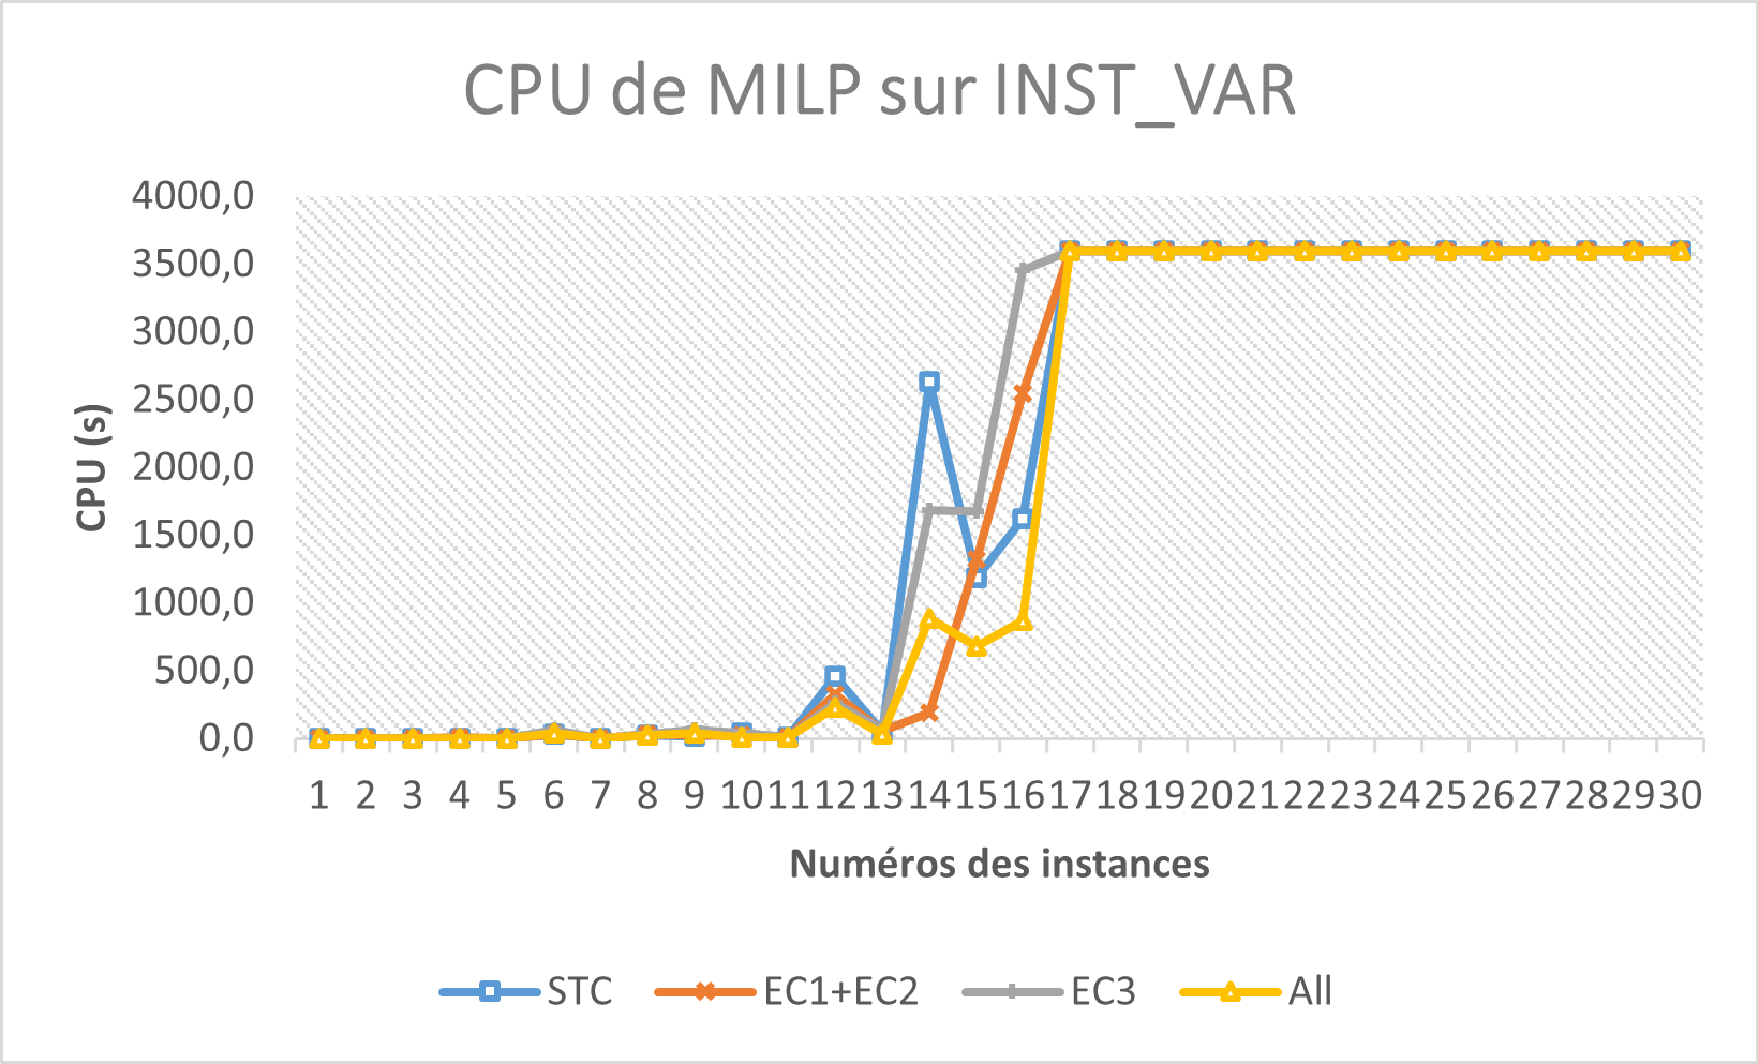
\includegraphics[width=\textwidth]{figures/CPU_MILP_INST_VAR.pdf}
    %\end{column}
    %\begin{column}{0.5\textwidth}
     % \centering
      %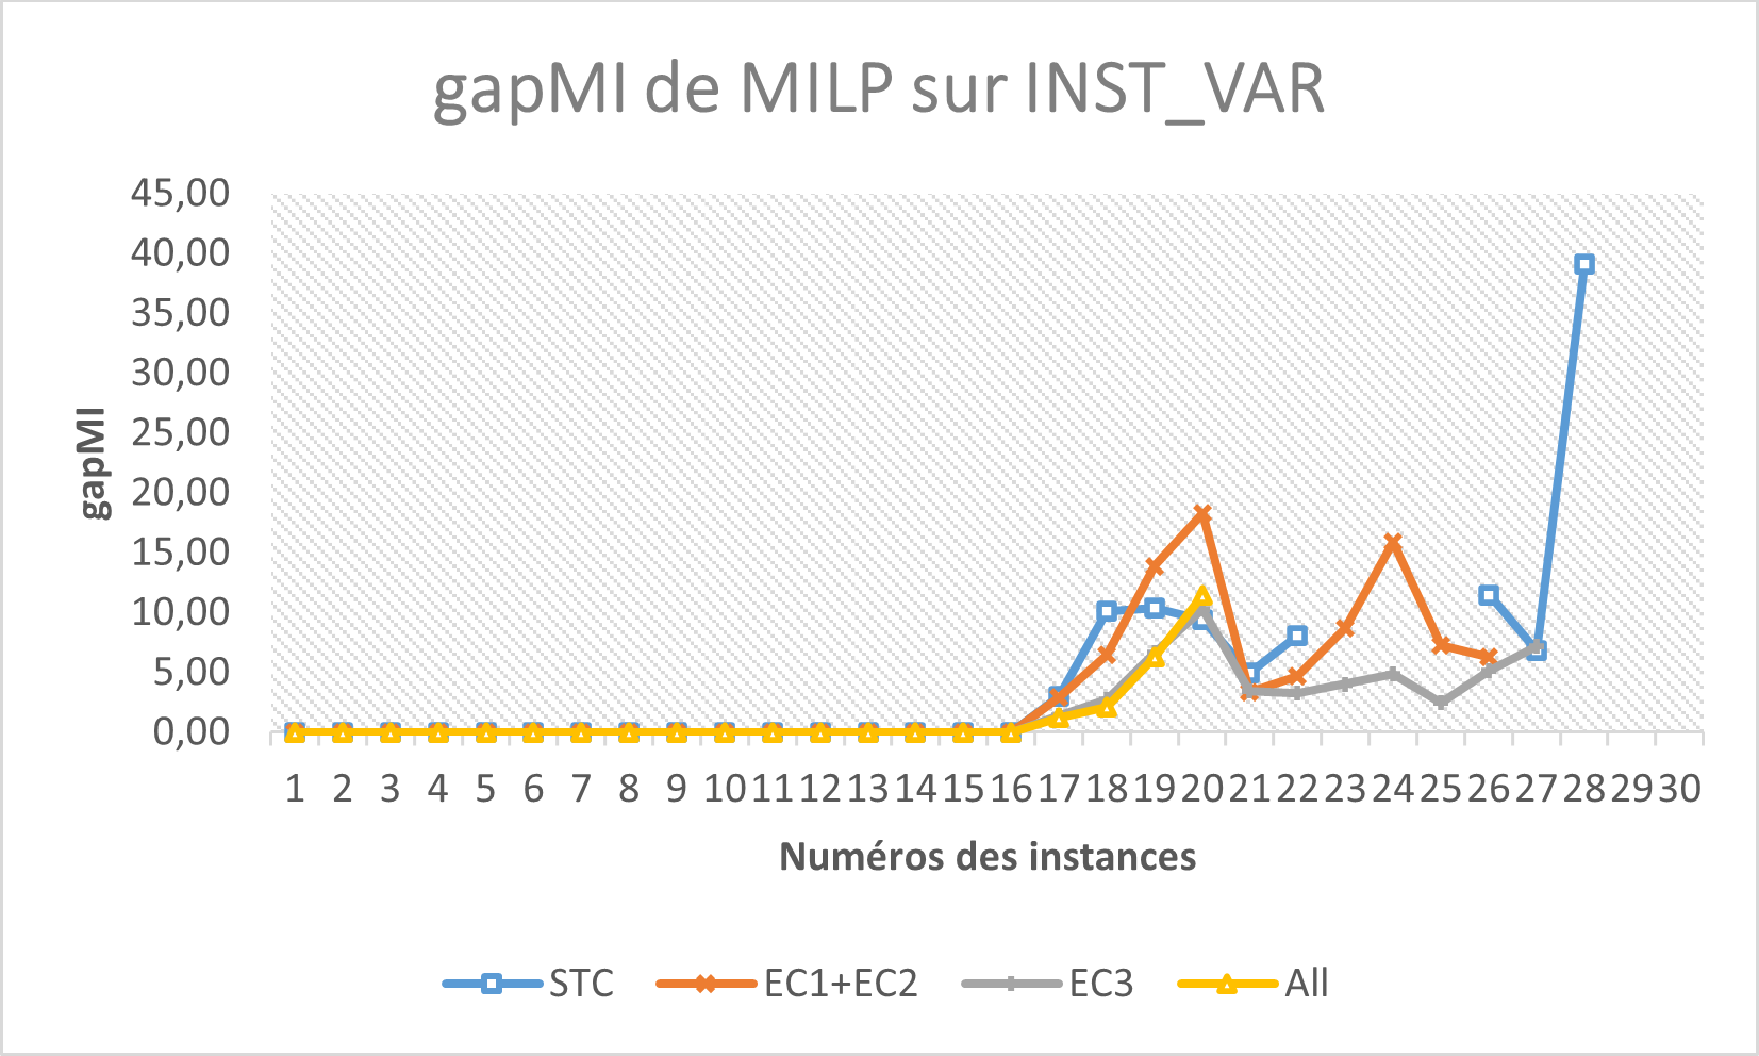
\includegraphics[width=\textwidth]{figures/gapMI_MILP_INST_VAR.pdf}
    %\end{column}
  %\end{columns}

  %\begin{columns}[onlytextwidth]
   % \begin{column}{0.5\textwidth}
    %  \centering
     % 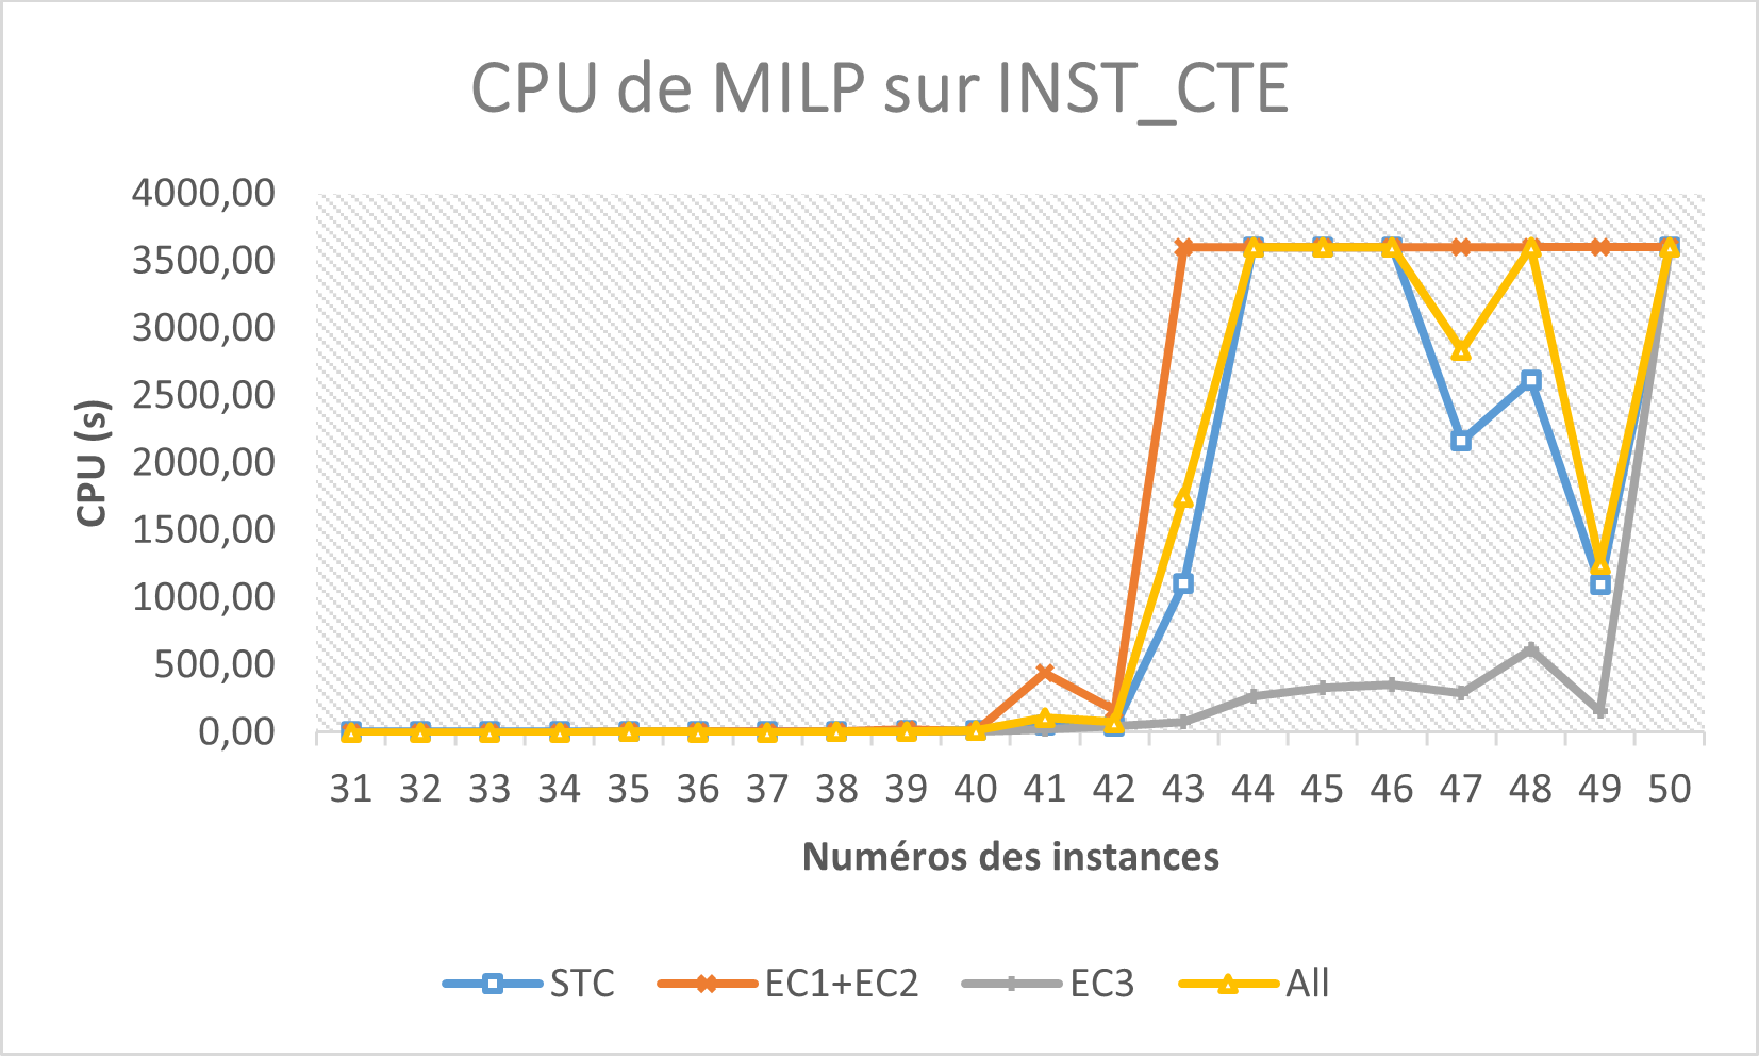
\includegraphics[width=\textwidth]{figures/CPU_MILP_INST_CTE.pdf}
    %\end{column}
    %\begin{column}{0.5\textwidth}
     % \centering
      %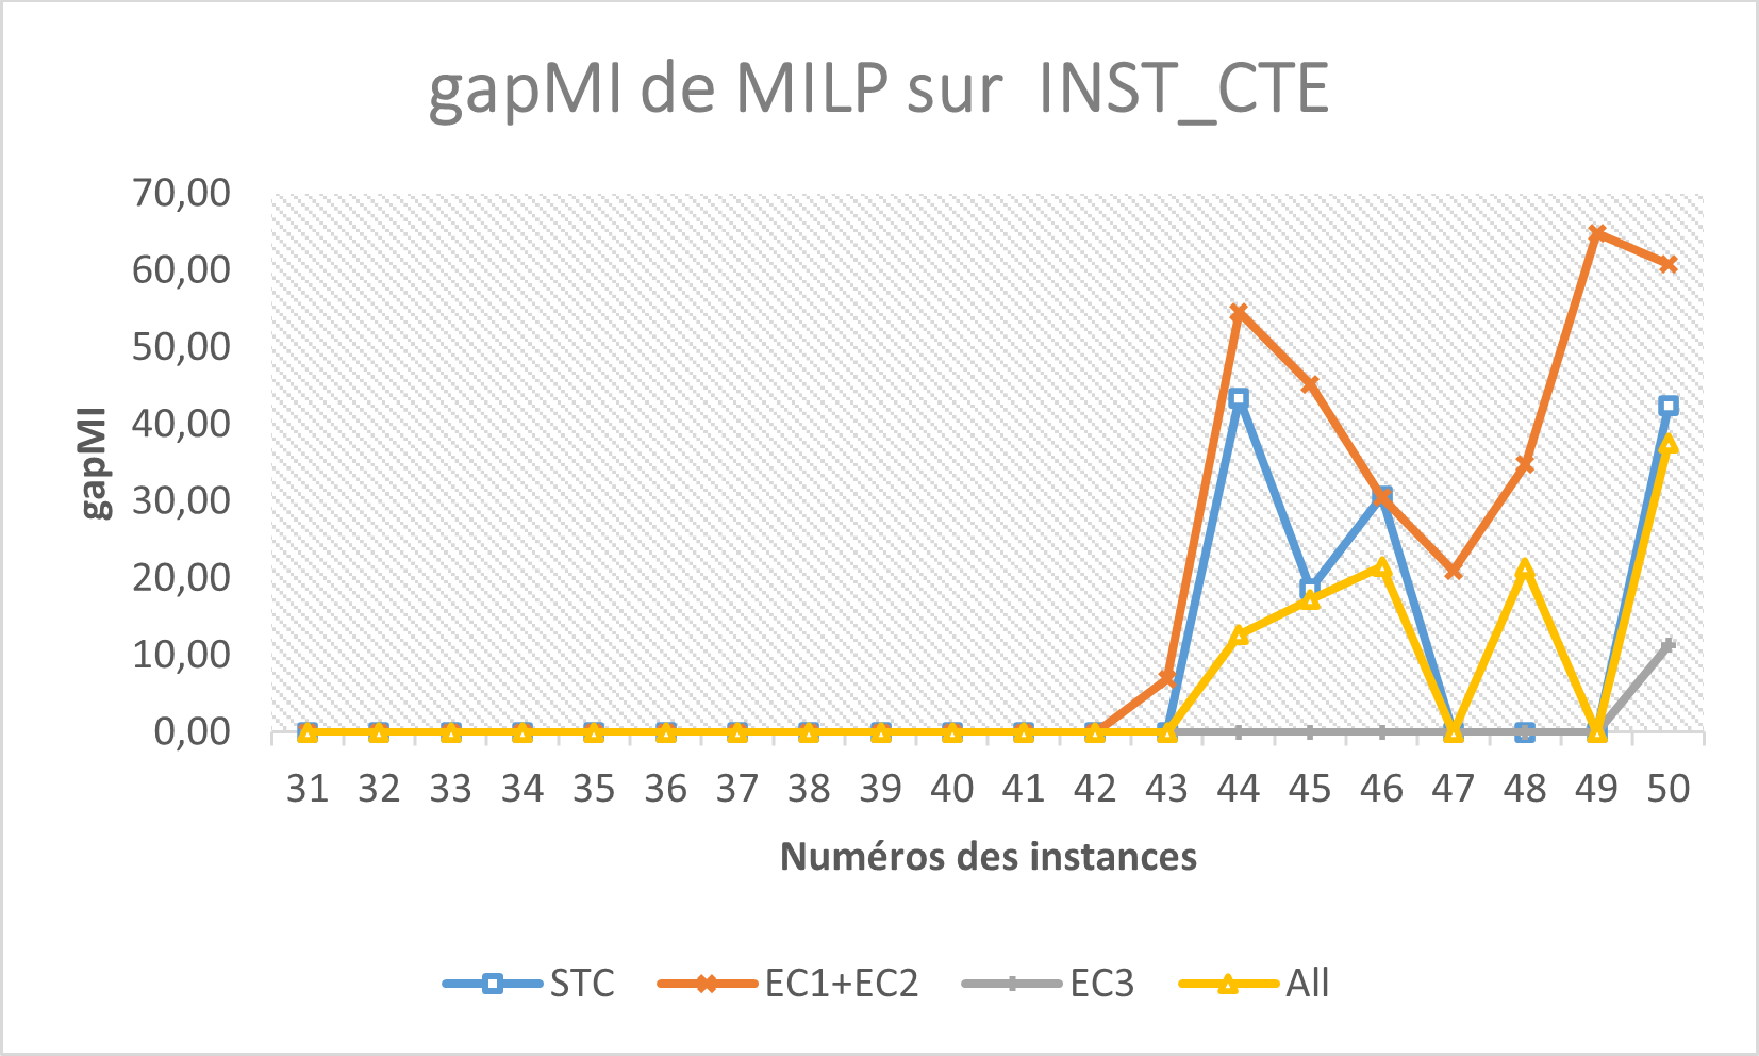
\includegraphics[width=\textwidth]{figures/gapMI_MILP_INST_CTE.pdf}
    %\end{column}
%  \end{columns}
%\end{frame}
%§§§§§§§§§§§§§§§§§§§§§§§§§§§§§§§§§§§§§§§§§§§§§§§§§§§
%\begin{frame}
%\frametitle{Expérimentations de MILP (1H)}% , \textit{mono-thread}) pour INST\_VAR

%\begin{itemize}
%\frametitle{Environnement}
%\item Gnu/linux Ubuntu 20.04.2, C++, CPLEX 12.10
%\item 30 instances
%\end{itemize}
%\begin{figure}[H]
%	\centering
%	\begin{tabular}{c c}
%		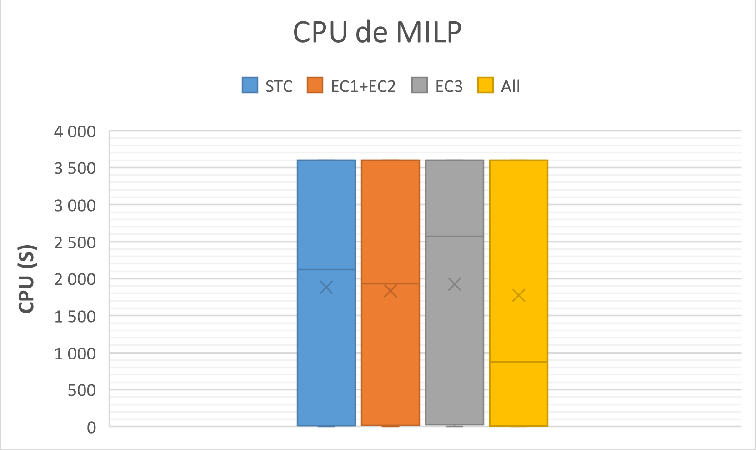
\includegraphics[width=6.5cm]{figures/slide_CPU_MILP_INST_VAR.pdf}&%CPU_MILP_INST_VAR
%		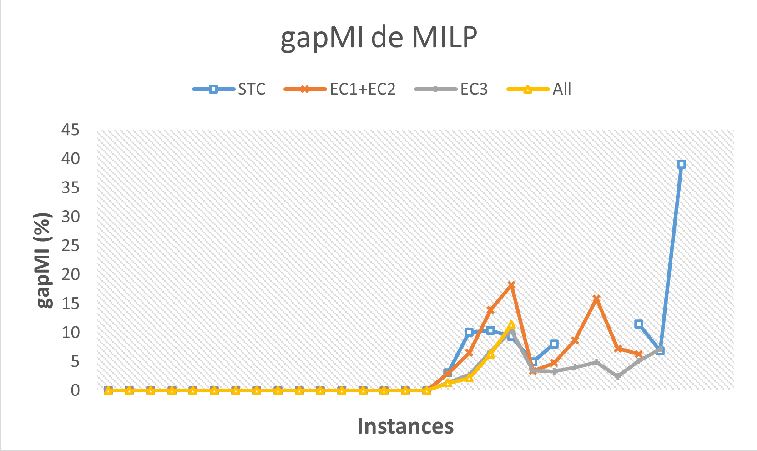
\includegraphics[width=6.5cm]{figures/slide_GAPMI_MILP_INST_VAR.pdf}%gapMI_MILP_INST_VAR
%		\\
%		(a) & (b)
%	\end{tabular}
%	\caption{ (a) représente le temps CPU et (b) représente le gap de chaque instance.}\label{gapMI_cpu_RMILP_INST_VAR}% de INST\_VAR.
%\end{figure}

%\end{frame}

%\begin{frame}
%\frametitle{MILP (1H, \textit{mono-thread}) pour INST\_CTE}
%\begin{figure}[H]
%	\centering
%	\begin{tabular}{c c}
%		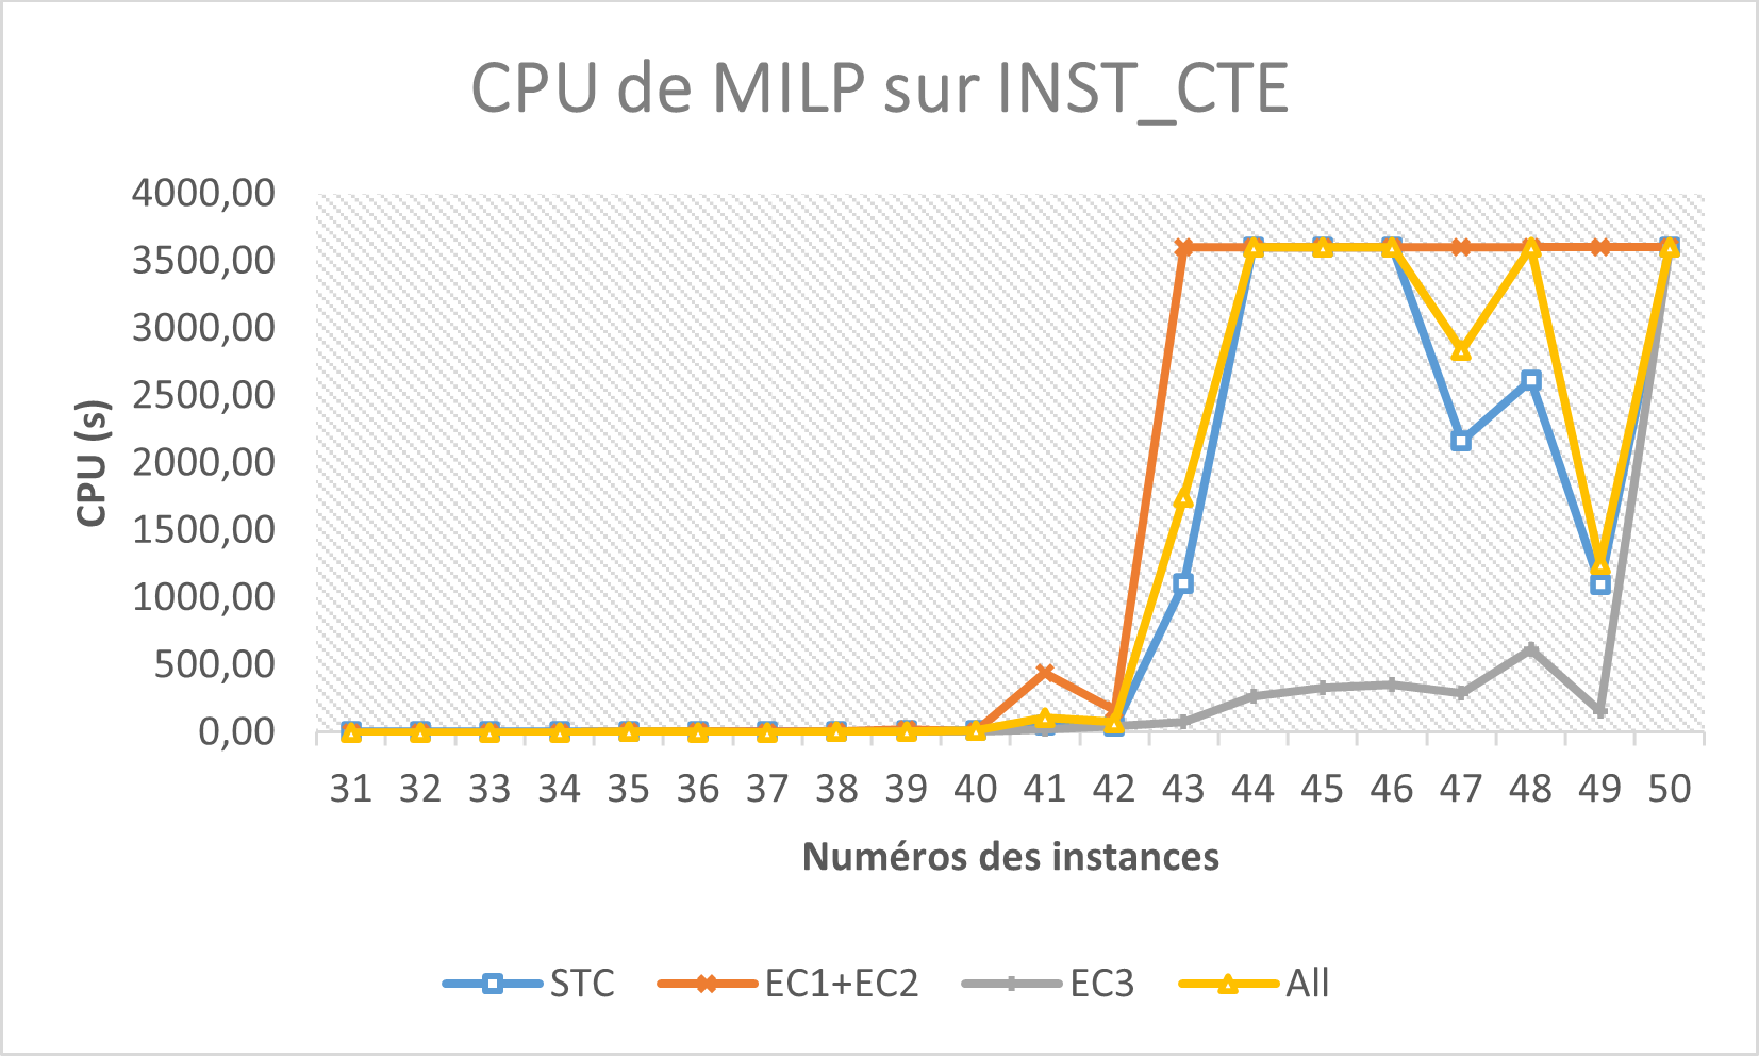
\includegraphics[width=6.5cm]{figures/CPU_MILP_INST_CTE.pdf}&
%		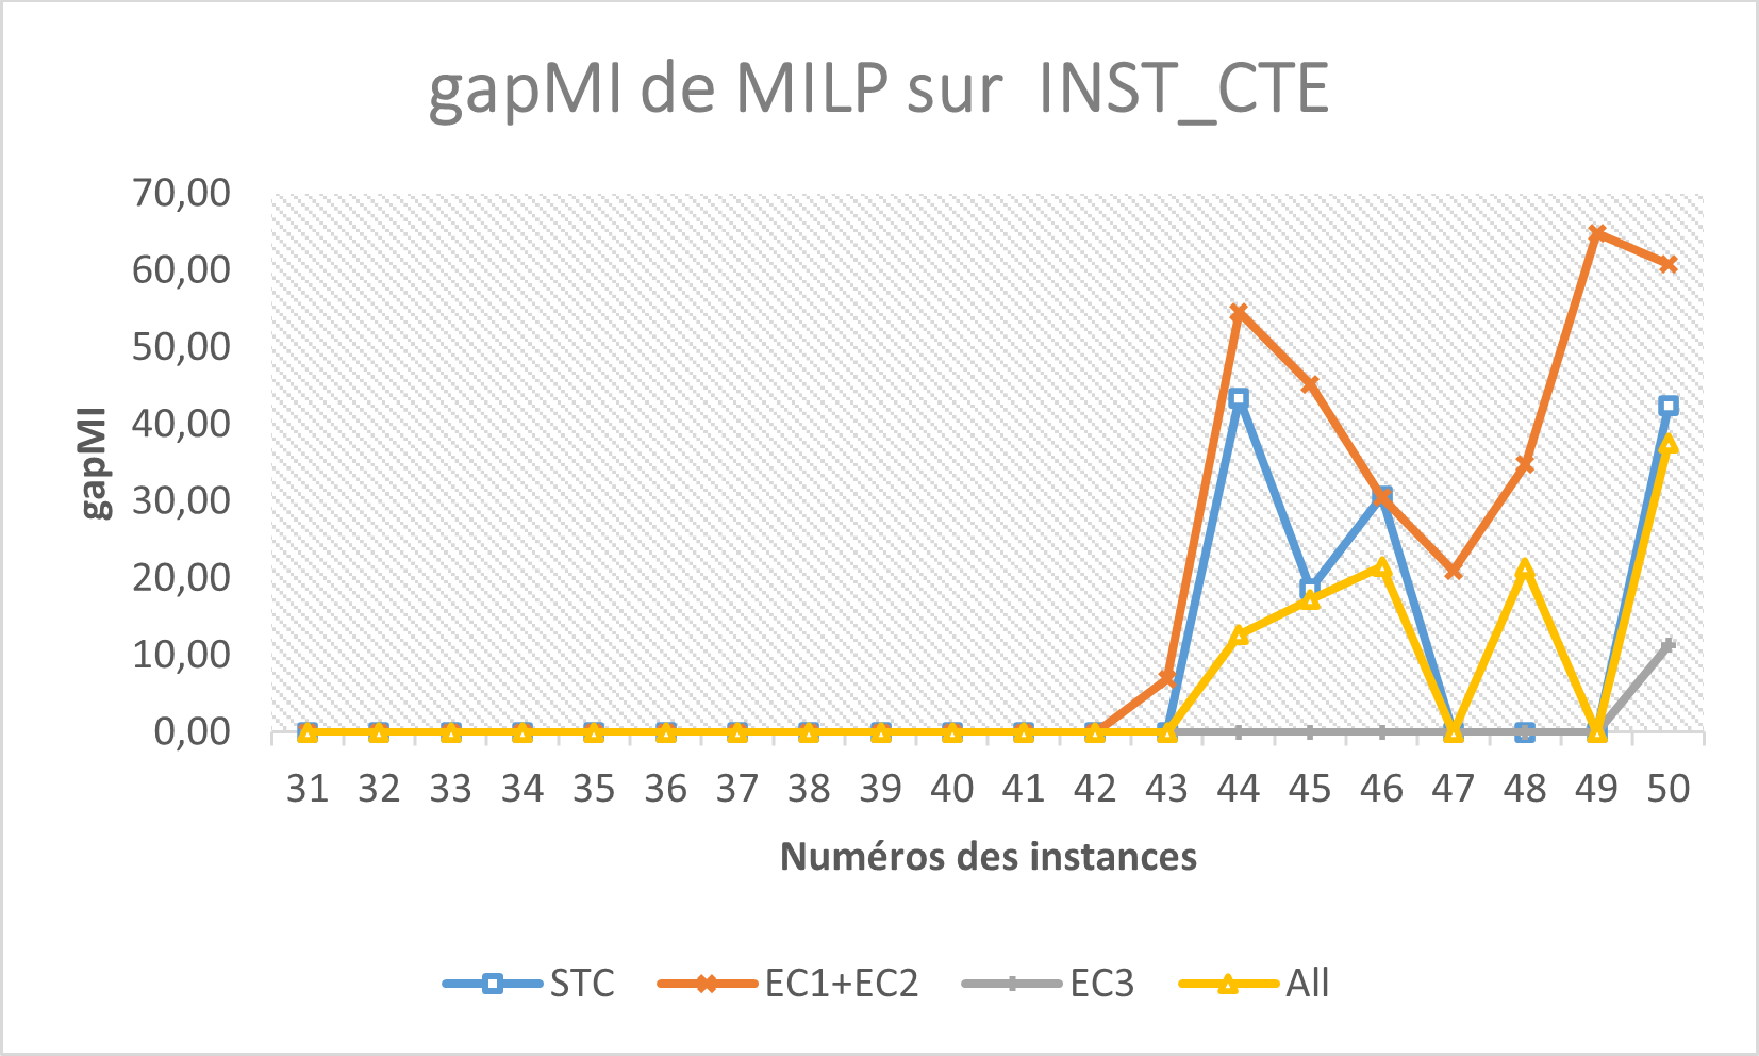
\includegraphics[width=6.5cm]{figures/gapMI_MILP_INST_CTE.pdf}
%		\\
%		(a) & (b)
%	\end{tabular}
%	\caption{(a) représente le temps CPU et (b) représente le gap pour chaque instance de INST\_CTE.}\label{gapMI_cpu_RMILP_INST_CTE}
%\end{figure}
%\end{frame}


%\begin{frame}
 % \frametitle{RMILP (1H, \textit{mono-thread}) pour INST\_VAR et INST\_CTE}

  %\begin{columns}[onlytextwidth]
  %  \begin{column}{0.5\textwidth}
   %   \centering
    %  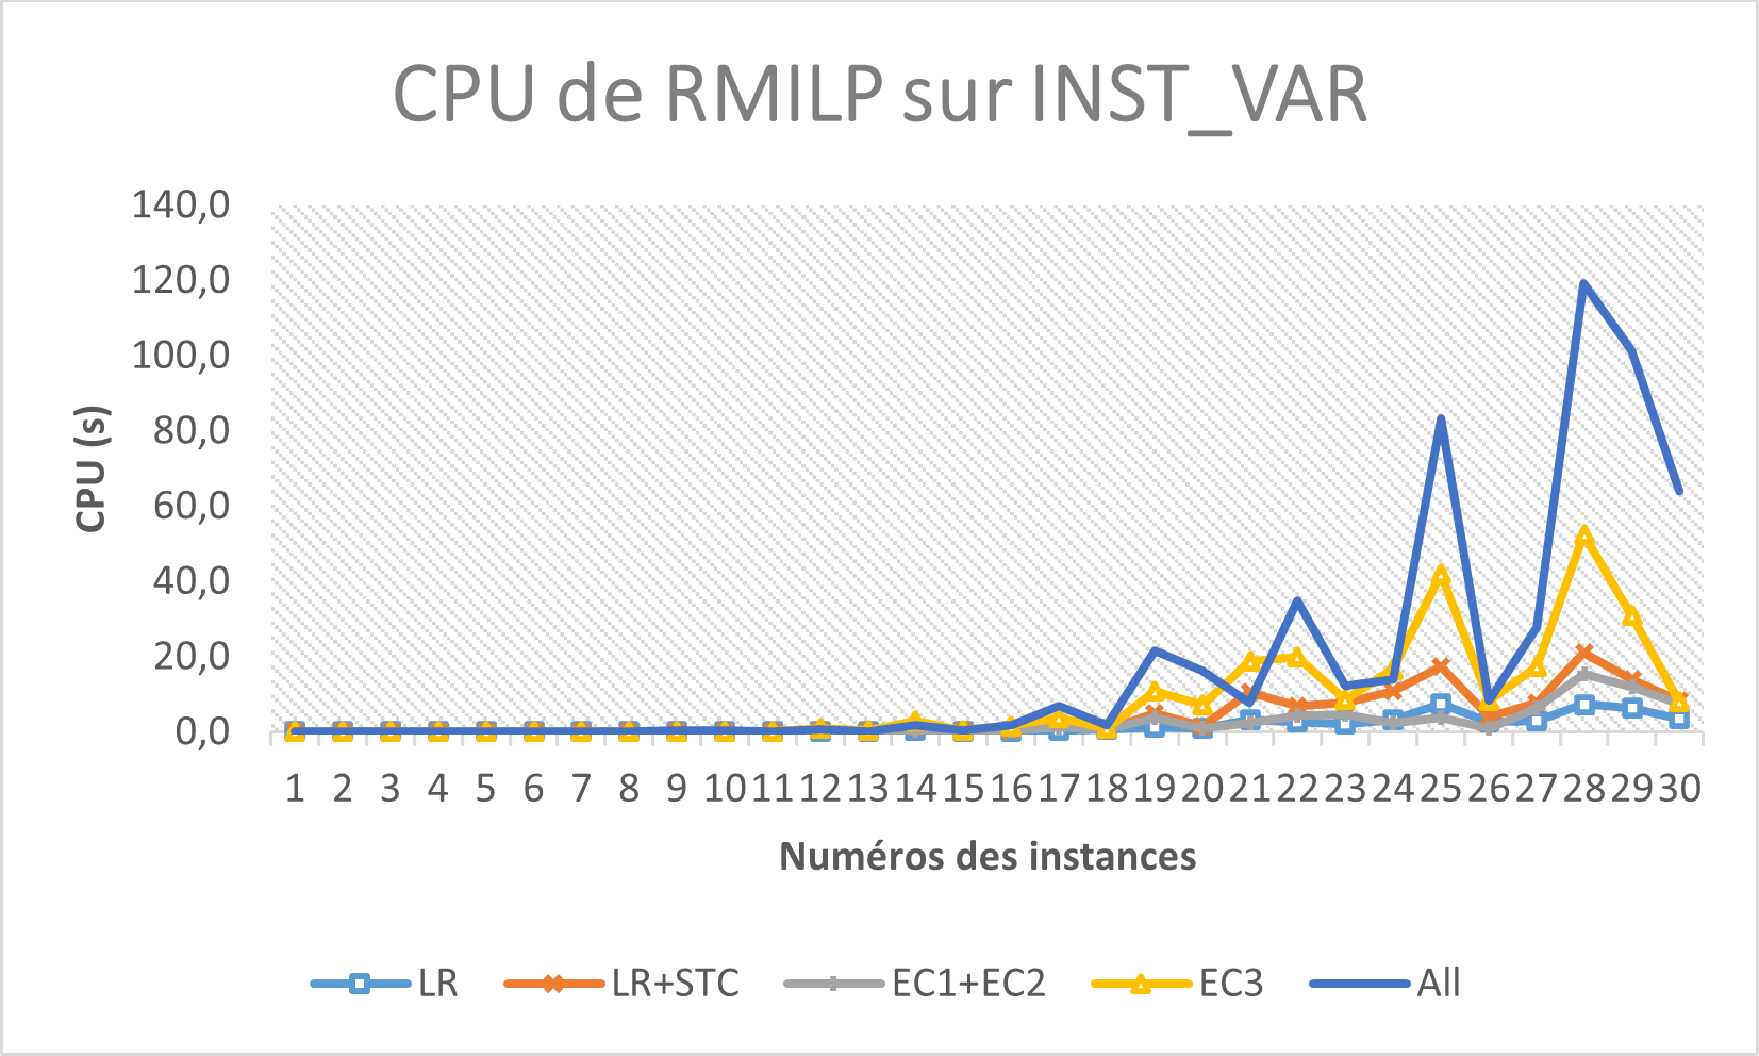
\includegraphics[width=\textwidth]{figures/CPU_RMILP_INST_VAR.pdf}
    %\end{column}
    %\begin{column}{0.5\textwidth}
     % \centering
     % 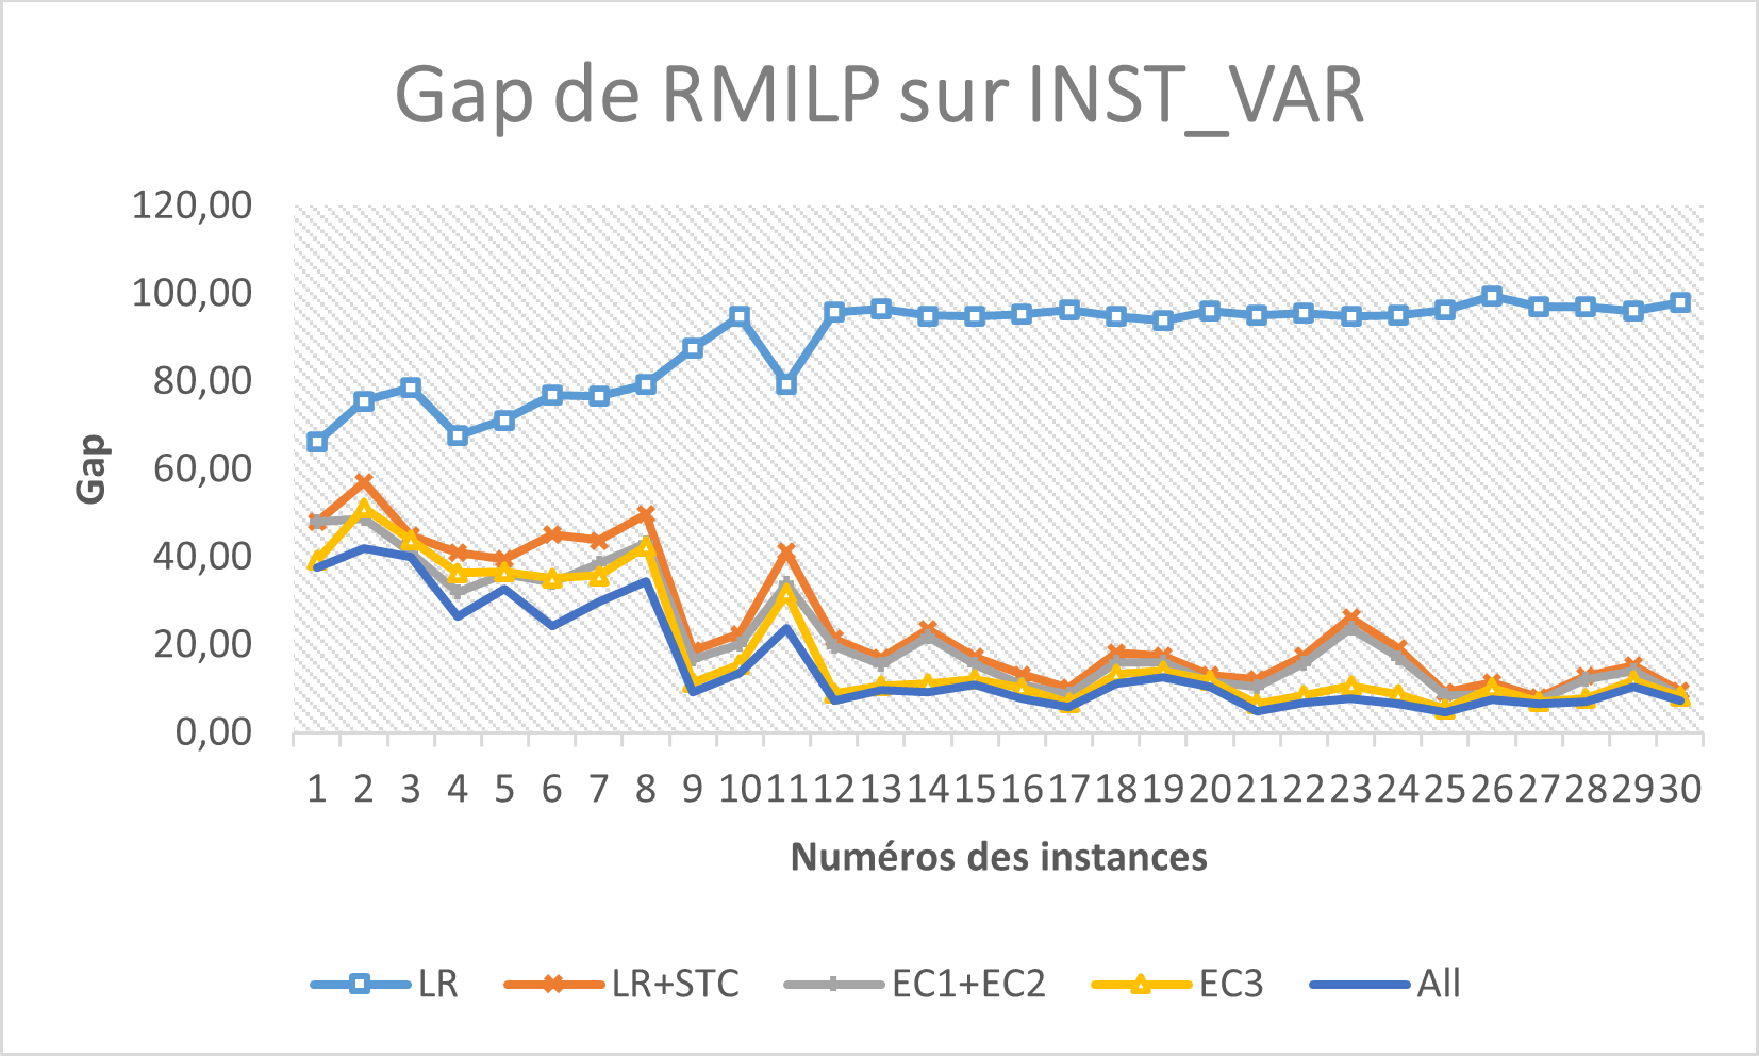
\includegraphics[width=\textwidth]{figures/Gap_RMILP_INST_VAR.pdf}
    %\end{column}
  %\end{columns}

  %\begin{columns}[onlytextwidth]
   % \begin{column}{0.5\textwidth}
    %  \centering
     % 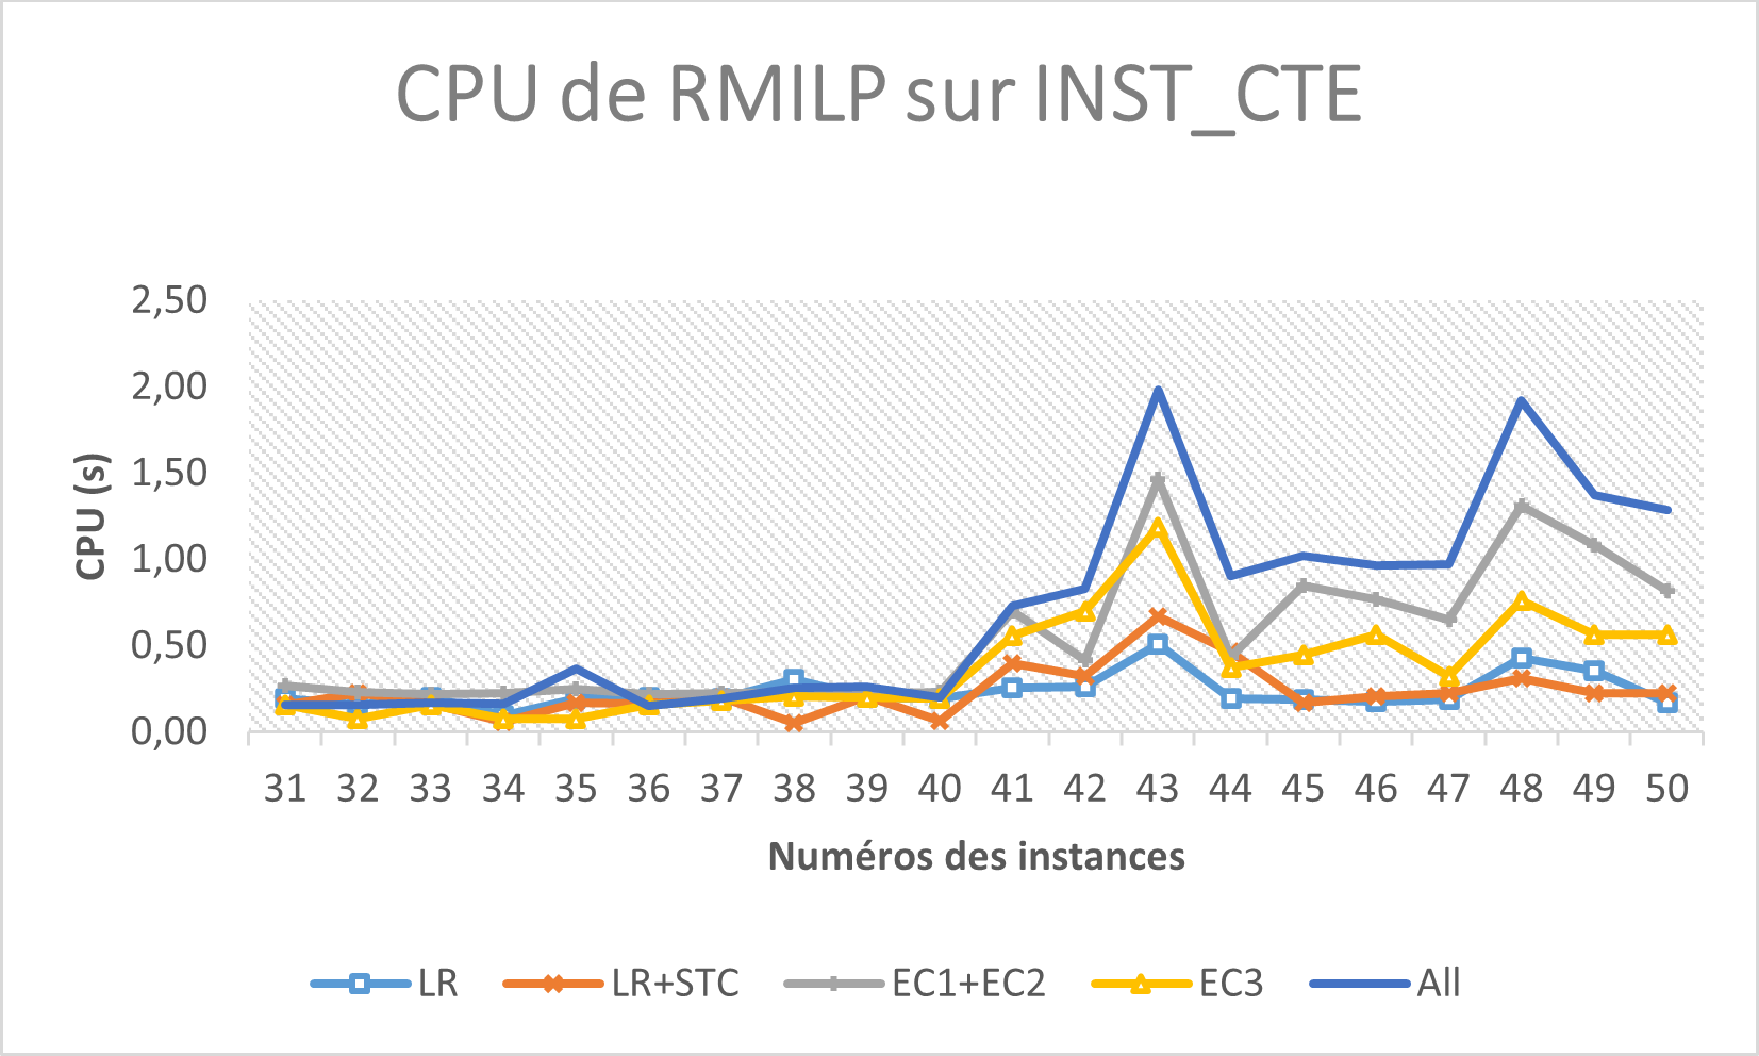
\includegraphics[width=\textwidth]{figures/CPU_RMILP_INST_CTE.pdf}
    %\end{column}
    %\begin{column}{0.5\textwidth}
     % \centering
      %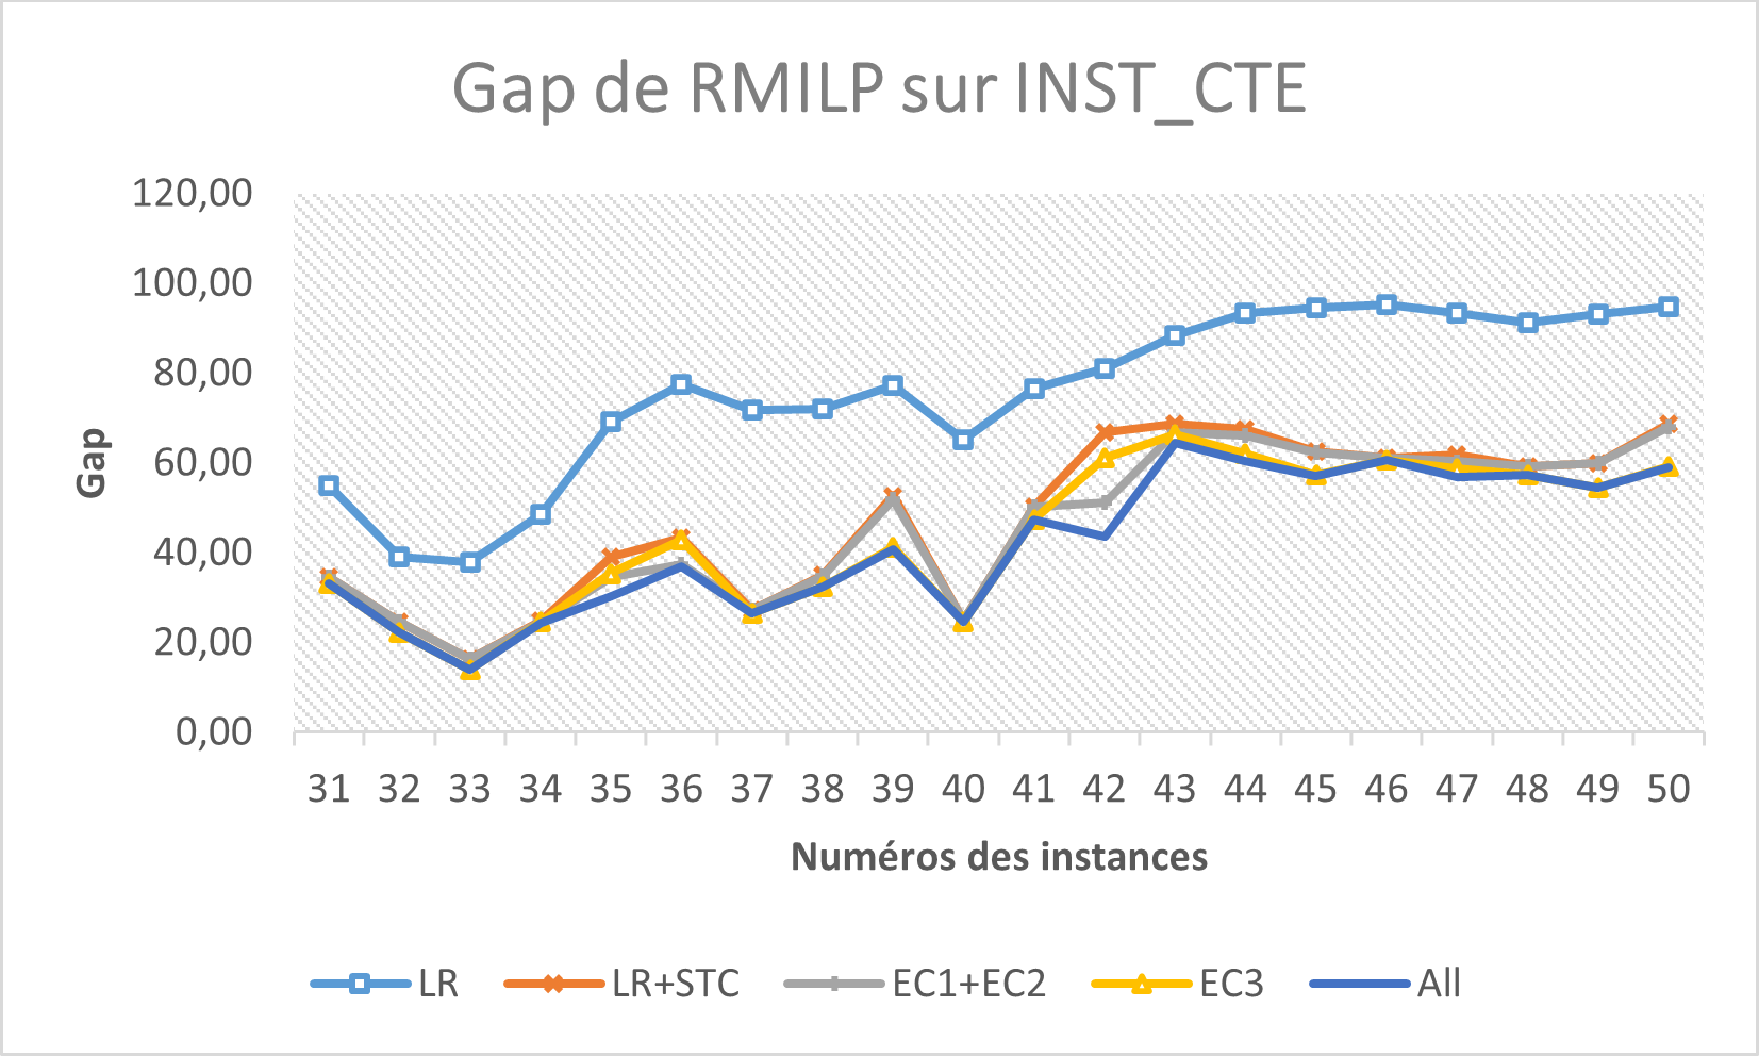
\includegraphics[width=\textwidth]{figures/Gap_RMILP_INST_CTE.pdf}
    %\end{column}
%  \end{columns}
%\end{frame}
%§§§§§§§§§§§§§§§§§§§§§§§§§§§§§§§§§§§§§§§§§§§§§§§§§§§

\begin{frame}
\frametitle{Expérimentations de la relaxation LR (1H)}%, \textit{mono-thread}) pour INST\_VAR
\begin{itemize}
\item Gnu/linux Ubuntu 20.04.2, C++, CPLEX 12.10
\item 30 instances. Solution de référence \textbf{BSup} : Borne supérieure de MILP (3H)
\item $Gap=100 \times \frac{\textbf{BSup}-Val}{\textbf{BSup}}$
\end{itemize}
\begin{figure}[H]
	\centering
	\begin{tabular}{c c}
		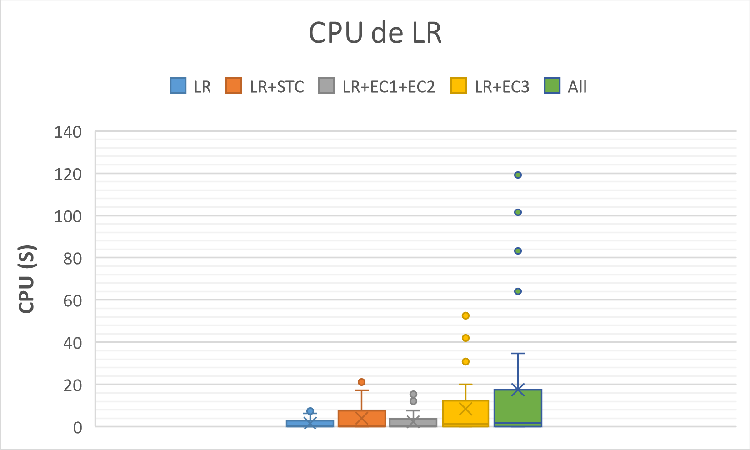
\includegraphics[width=6.5cm]{figures/slide_CPU_RMILP_INST_VAR.pdf}&%CPU_RMILP_INST_VAR.pdf
		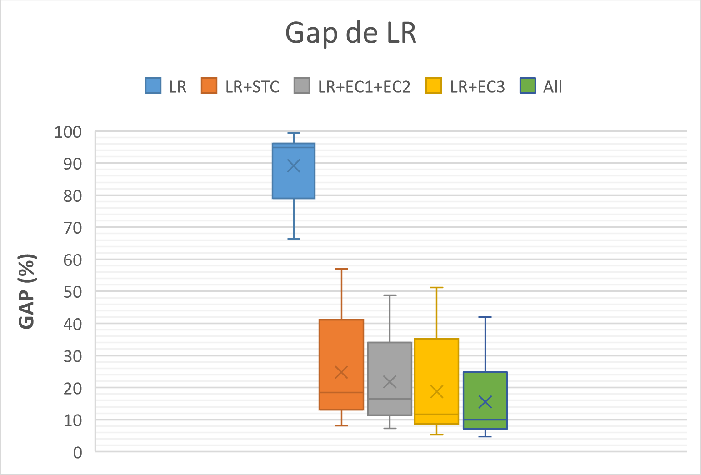
\includegraphics[width=6.5cm]{figures/slide_GAP_RMILP_INST_VAR.pdf}%Gap_RMILP_INST_VAR.pdf
		\\
		(a) & (b)
	\end{tabular}
	\caption{ (a) représente le temps CPU et (b) représente le gap de chaque modèle.}\label{gap_cpu_RMILP_INST_VAR}% de INST\_VAR
\end{figure}

\end{frame}
%\begin{frame}
%\frametitle{RMILP (1H, \textit{mono-thread}) pour INST\_CTE}
%\begin{figure}[H]
%	\centering
%	\begin{tabular}{c c}
%		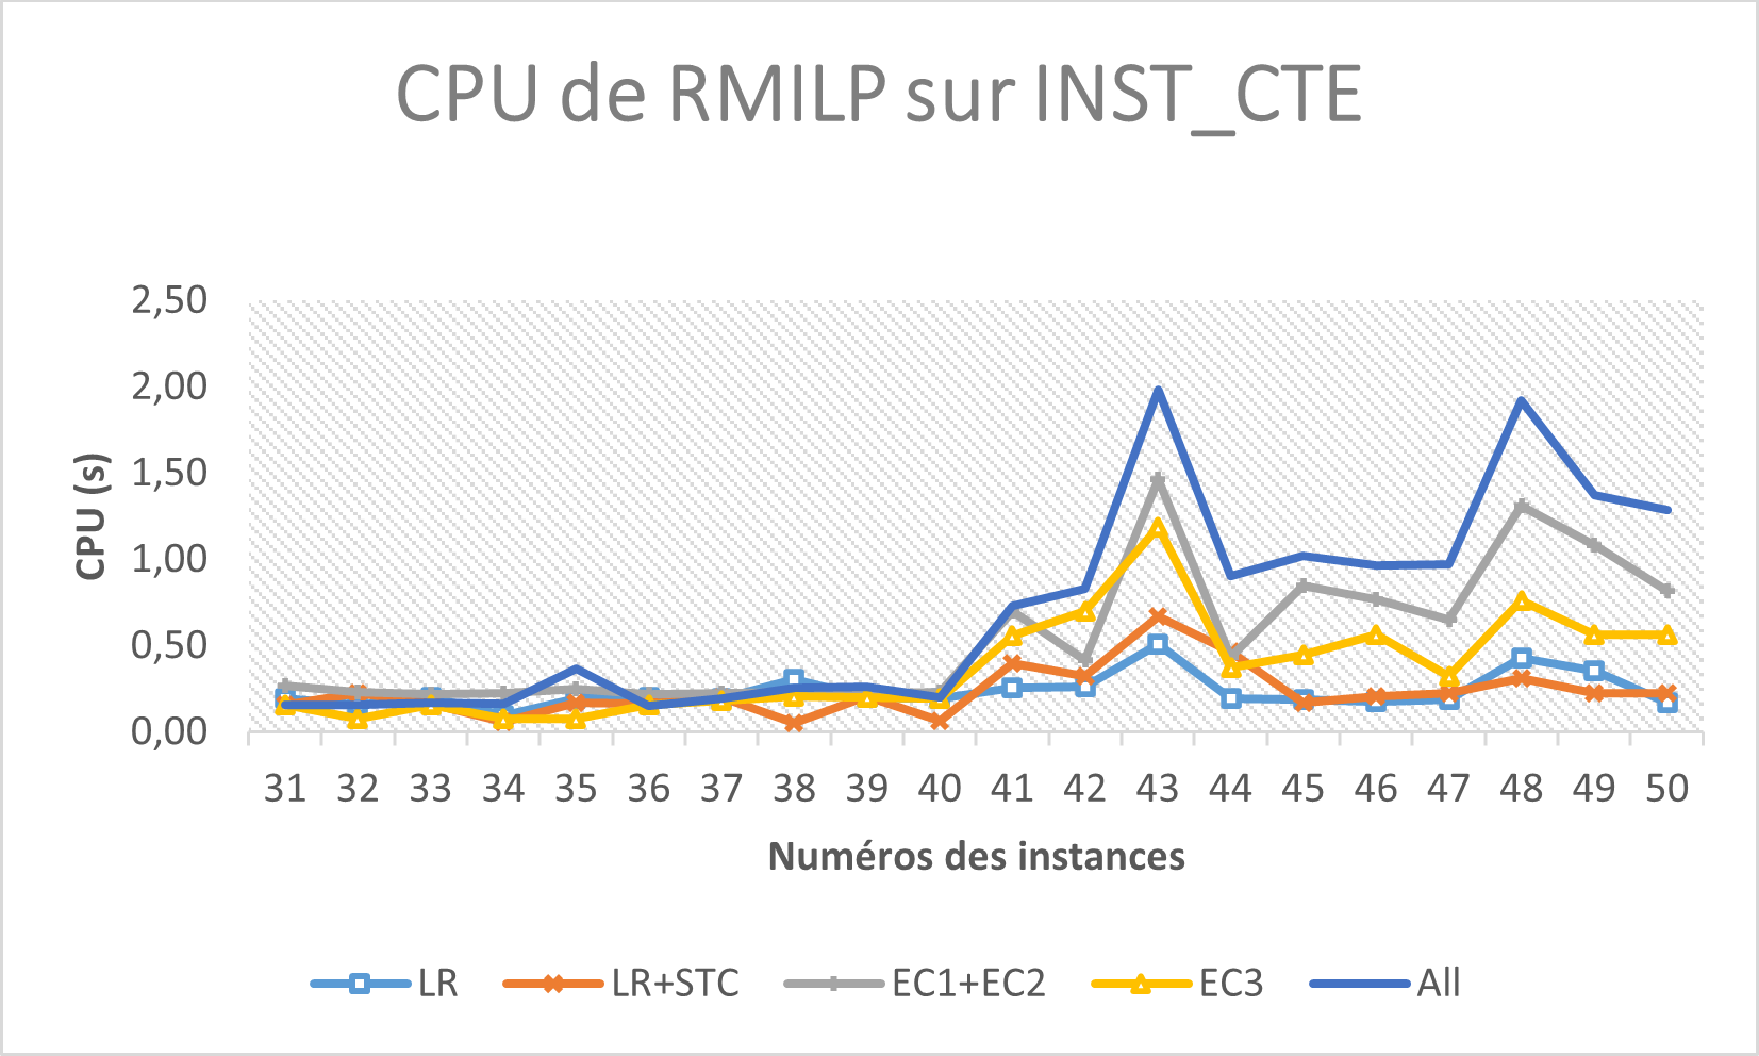
\includegraphics[width=6.5cm]{figures/CPU_RMILP_INST_CTE.pdf}&
%		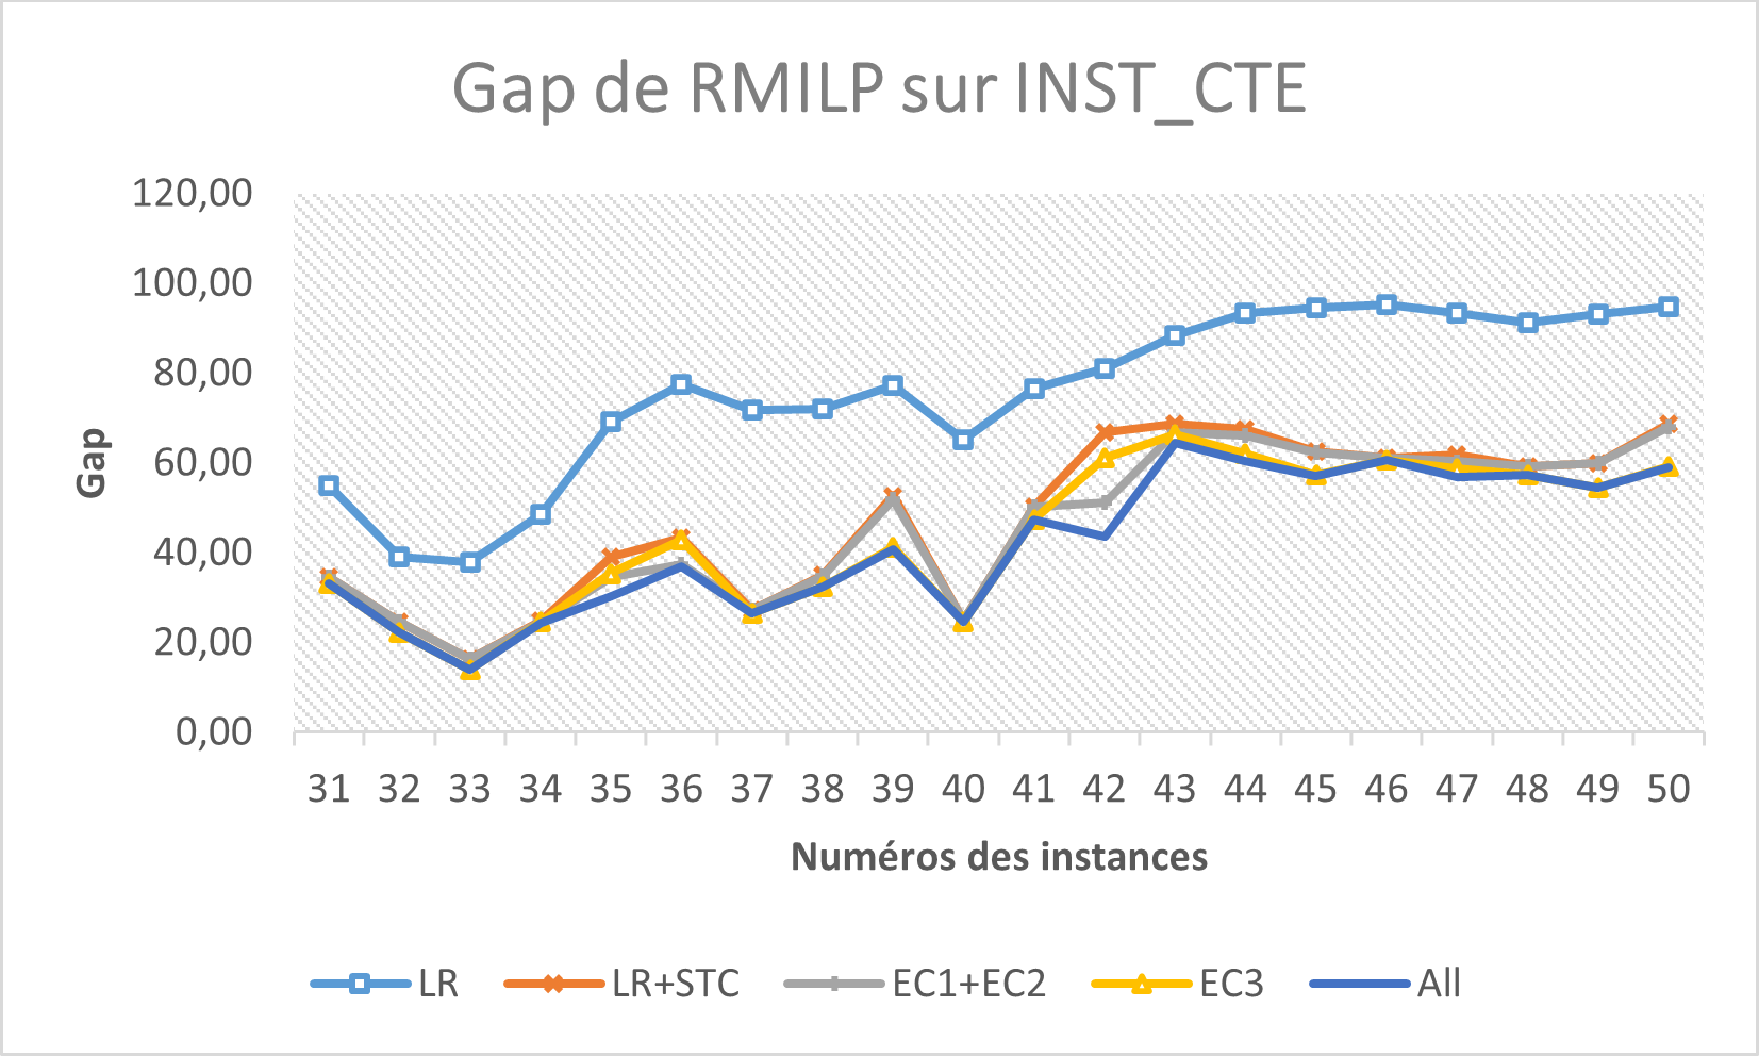
\includegraphics[width=6.5cm]{figures/Gap_RMILP_INST_CTE.pdf}
%		\\
%		(a) & (b)
%	\end{tabular}
%	\caption{(a) représente le temps CPU et (b) représente le gap pour chaque instance de INST\_CTE.}\label{gap_cpu_RMILP_INST_CTE}
%\end{figure}
%\end{frame}
\subsection{Programmation dynamique \textbf{\textit{DPS\_SMEPC}}}
\begin{frame}
\frametitle{Plan}
\addtocounter{framenumber}{-1}
\tableofcontents[currentsection,currentsubsection]
\end{frame}

\begin{frame}
	\frametitle{Programmation dynamique (1/4) : rappel}
 \begin{figure}
	\centering
   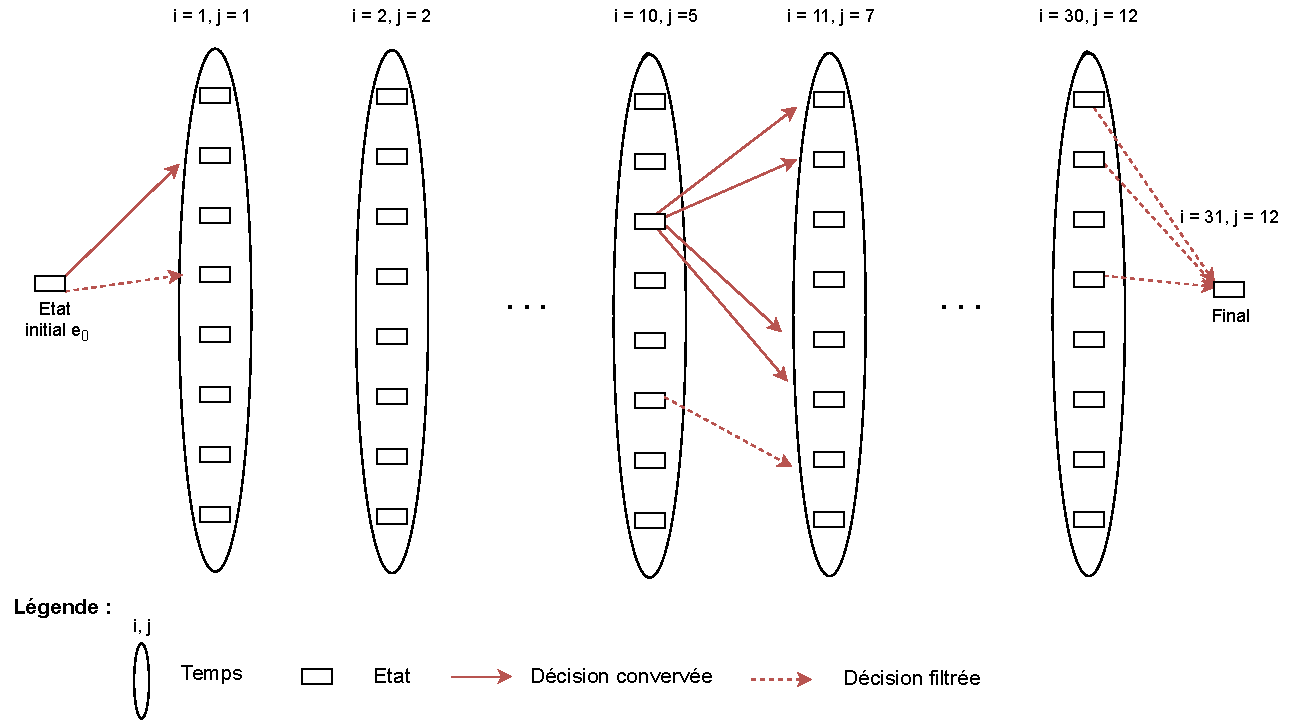
\includegraphics[width=\textwidth]{./figures/slide_Fr_Structure_G.pdf}
	%\caption[Structure Générale du Réseau d'État "Production" ]{Structure Générale du Réseau d'État «Production».}
	\label{Structure_G}
\end{figure}
 \end{frame}
\begin{frame}
	\frametitle{Programmation dynamique (2/4) : temps, états, décisions}
 


\begin{minipage}{.4\textwidth}%

\begin{figure}
    \centering
   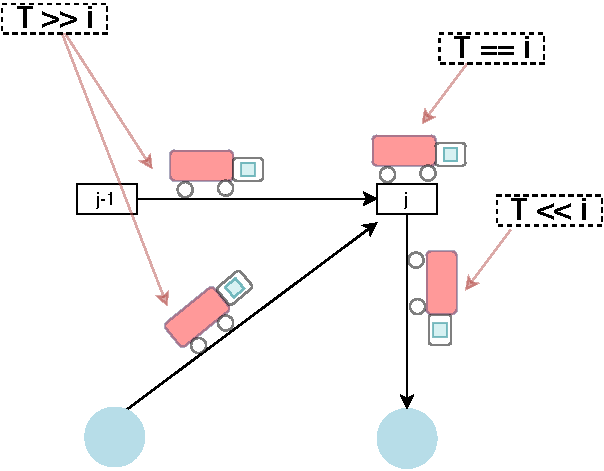
\includegraphics[width=\textwidth]{./figures/positions_vehicule.pdf}%exalgopdf(4)
   \caption{Exemple de décision du problème.}
   \label{fig:my_label}
\end{figure}

\end{minipage}%
\hfill
\begin{minipage}{.6\textwidth}%
\begin{enumerate}
\item Temps DPS (Dynamic Programming Schema)
\begin{itemize}
\item Temps station ($j$) ;
\item Temps usine ($i$).

\end{itemize}
\item Etats %($[i-1,i]$)
\begin{itemize}
%\item Station $i$ sur laquelle le véhicule se trouve
\item \'{E}tat de la micro-usine ($Z$) ;
\item Date d'arrivée du véhicule en $j$ ($T$) ;
\item Citerne ($V^{Tank}$) ;

\item Réservoir du véhicule ($V^{Veh}$).



\end{itemize}
\item Décisions %($[i,i+1]$)
\begin{itemize}
\item Décision de recharger($x$) ;
\item Décision de produire ($z$) ;
\item Choix période de recharge ($\delta$).
\end{itemize}
%\item $\sum_{t=0 \dots N-1} (C_f.q_t+C_t .z_t) + \lambda.T_{n+1}$

\item Etat initial $i=0$, $j=0$ : (0,0,$H_0$,$E_0$)
\item Etats finaux $i\leq N$, $ j=M+1$: $(Z,T\leq TMax; V^{Tank} \geq H_0; V^{Veh} \geq E_0)$ %(\textit{Forward})

\end{enumerate}
\end{minipage}%

\end{frame}
\begin{frame}
	\frametitle{Programmation dynamique (3/4) : Exemple}

\begin{table}[H]
	\centering
	\begin{tabular}{|c|c||c|c|c|c||c||c|c|c|}
		%\hline
	%\rowcolor{cyan}	\multicolumn{2}{|c||}{temps DPS (i,j)}& \multicolumn{4}{|c||}{Etat $s = (Z, T, V^{Tank}, V^{Veh})$}&Coût $ W$ & \multicolumn{3}{|c|}{Décisions $ D = (z, x, \delta )$ } \\
		\hline
		i & j & Z &T & $V^{Tank}$ & $V^{Veh}$&W=Cost + T & z & x&$\delta$ \\ 
		\hline
		0 & 0 & 0 &0 & 4 & 8&0 + 0 & 0 & \textcolor{greenn}{0}&0 \\ 
		\hline
		1 &\textcolor{greenn}{1} & 0 &\textcolor{greenn}{4} & 4 & \textcolor{greenn}{3}&0 + \textcolor{greenn}{4} & \textcolor{blue}{1} & 0&0 \\ 
		\hline
		2 &1 & \textcolor{blue}{1} &4 & \textcolor{blue}{9} & 3&\textcolor{blue}{8} + 4 & 1 & 1&0 \\ 
		\hline
		3 &1 & 1 &4 & 13 & 3&9 + 4 & 0 &0&0 \\ 
		\hline
		4 &1 & 0 &4 & 13 & 3&9 + 4 & 0 & 0&\textcolor{red}{1} \\ 
		\hline
		5 &\textcolor{red}{2} & 0 &\textcolor{red}{12} & \textcolor{red}{0} & \textcolor{red}{12}&9 + \textcolor{red}{12} & 1 & 0&0 \\ 
		\hline
		%6&	3&	1&	19&	3&	9&	18 + 19&	1&	0&	0\\
		%\hline
		%7&	3&	1&	19&	8&	9&	20 + 19	&1	&0	&0\\
		%\hline
		%8&	3&	1&	19&	12&	9&	22 + 19	&0	&0	&0\\
		%\hline
  %		9&	3&	0&	19&	12&	9&	22 + 19&	0&	1&	0\\
	%	\hline
	%	10&	3&	0&	19&	12&	9&	22 + 19	&0	&0	&0\\
	%	\hline
	%	11&	3&	0&	19&	12&	9&	22 + 19&	0&	0&	0\\
	%	\hline
	%	12&	3&	0&	19&	12&	9&	22 + 19&	0&	0&	1\\
	%	\hline
	%	13&	4&	0&	27&	0&	12&	22 + 27	&1  &0	&0\\
	%	\hline
	%	14&	5&	1&	29&	4&	10&	30 + 29	&0&	0	&0\\
		%\hline
		%15&	6&	0&	30&	4&	8&	30 + 30	&*&	*	&*\\

		\hline
		
	\end{tabular}
	%\caption[Simulation de l'évolution du temps DPS]{Simulation de l'évolution du temps $(i,j)$, $s$, $D$ et $Cost + \alpha \times T$ correspondant à la figure (\ref{Synchro_exemple}). }
	\label{Simulation_synchro}
\end{table}

\begin{figure}
	\centering
   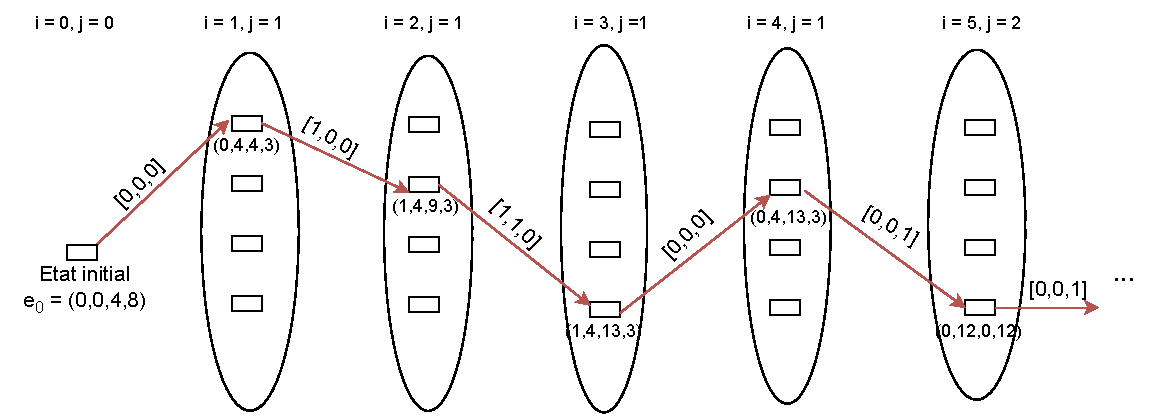
\includegraphics[width=11.8cm]{./figures/slide_exemple_Fr_Structure_G.pdf}
	%\caption[Structure Générale du Réseau d'État "Production" ]{Structure Générale du Réseau d'État «Production».}
	\label{exemple_Structure_G}
\end{figure}

\end{frame}


%\begin{frame}
%	\frametitle{Programmation dynamique (2/2) : règles de filtrage}
%	\begin{enumerate}
%	\item Règles de filtrage
% \begin{itemize}
%\item	Relations de dominance (\textbf{C})


%\item Filtrage par la réalisabilité : basé sur l’anticipation des incohérences (\textbf{A})


%\item	Filtrage par la borne supérieure (\textbf{B}) : sur la base du pré-calcul d'une solution initiale réalisable
% \end{itemize}
% \begin{figure}
 %   \centering
%   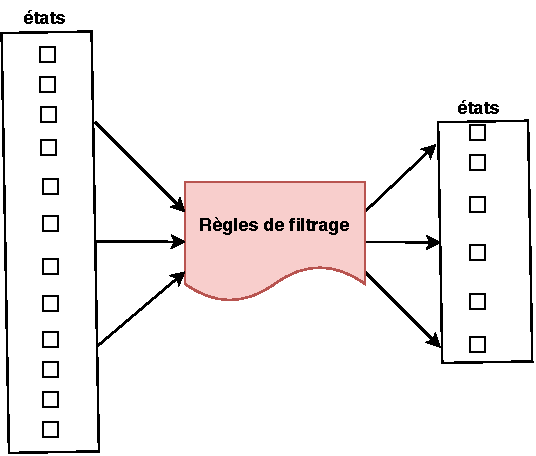
\includegraphics[scale=0.5]{./figures/Filtrage.pdf}
%    \caption{Impact des règles de filtrage sur le nombre d'états.}
 %   \label{fig:my_label}
%\end{figure}
% \item Approche heuristique : sélection des NS meilleurs états
 %\end{enumerate}
%\end{frame}


\begin{frame}
	\frametitle{DPS\_SMEPC (4/4) : règles de filtrage}


\begin{minipage}{.5\textwidth}%

\begin{figure}
    \centering
   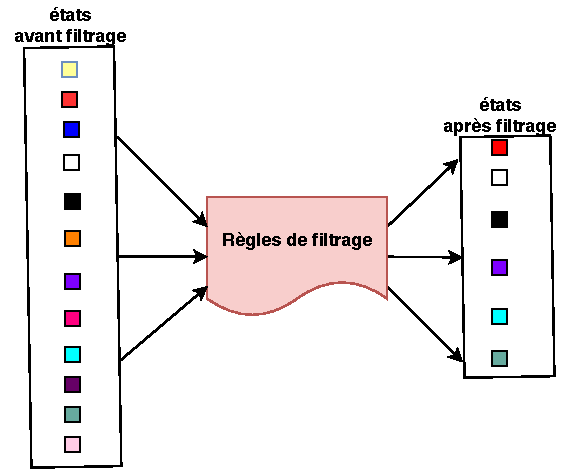
\includegraphics[width=\textwidth]{./figures/Filtrage(1).pdf}
    \caption{Impact des règles de filtrage sur le nombre d'états.}
    \label{fig:my_label}
\end{figure}

\end{minipage}%
\hfill
\begin{minipage}{.5\textwidth}%

	%\begin{enumerate}
	%\item
 Règles de filtrage :
 \begin{itemize}

\item \textbf{sans\_F} : Sans filtrage ;%ST(1)

\item \textbf{F\_logique} : Filtrage logique (suppression d'états si pas assez de temps ou d’énergie pour que le véhicule puisse finir sa
tournée) ;%ST(2) %(estimation de la durée et de l'énergie minimal necessaire pour finir la tournée plus petit respectivement que $TMax$ et l'énergie total stockée et produite;

\item \textbf{F\_optimiste} : F\_logique + Filtrage par estimation optimiste.%ST(3)
 \end{itemize}
 
 
% \end{enumerate}
\end{minipage}%

\end{frame}




%\begin{frame}
%  \frametitle{\textbf{DPS\_SMEPC} pour INST\_VAR et INST\_CTE}

 % \begin{columns}[onlytextwidth]
  %  \begin{column}{0.5\textwidth}
   %   \centering
    %  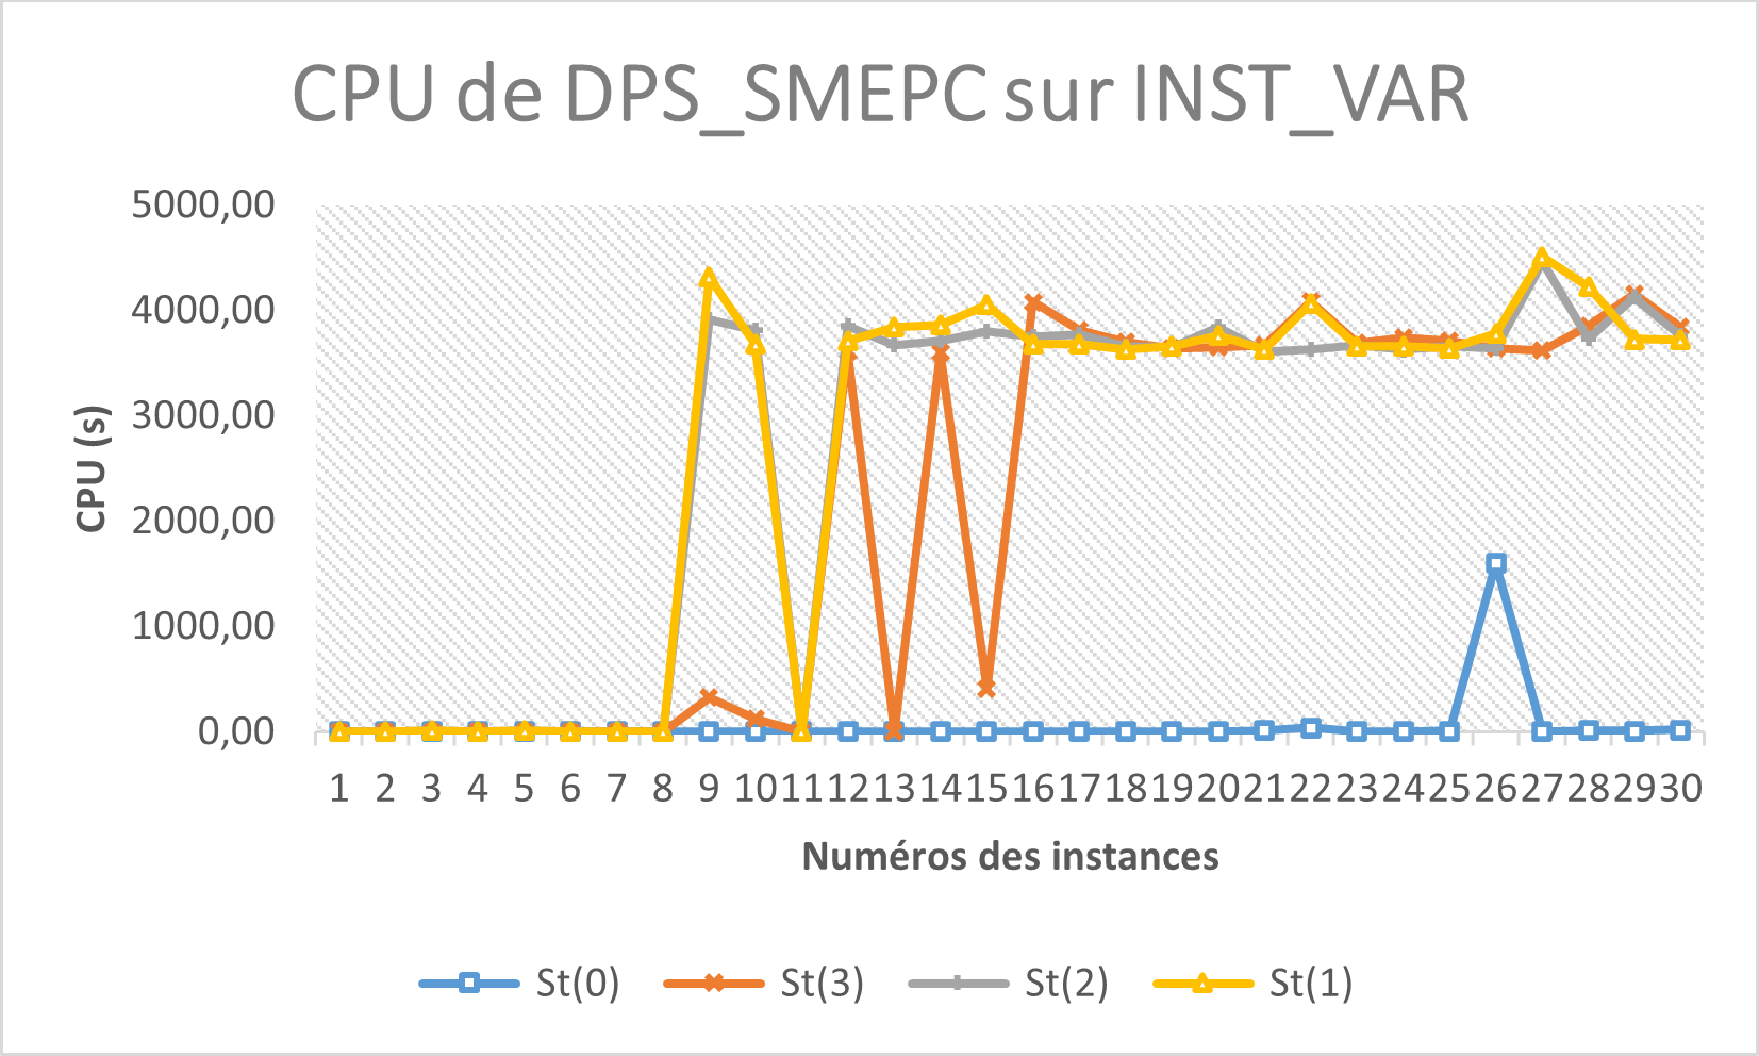
\includegraphics[width=\textwidth]{figures/CPU_DPS_SMEPC_INST_VAR.pdf}
%    \end{column}
 %   \begin{column}{0.5\textwidth}
  %    \centering
   %   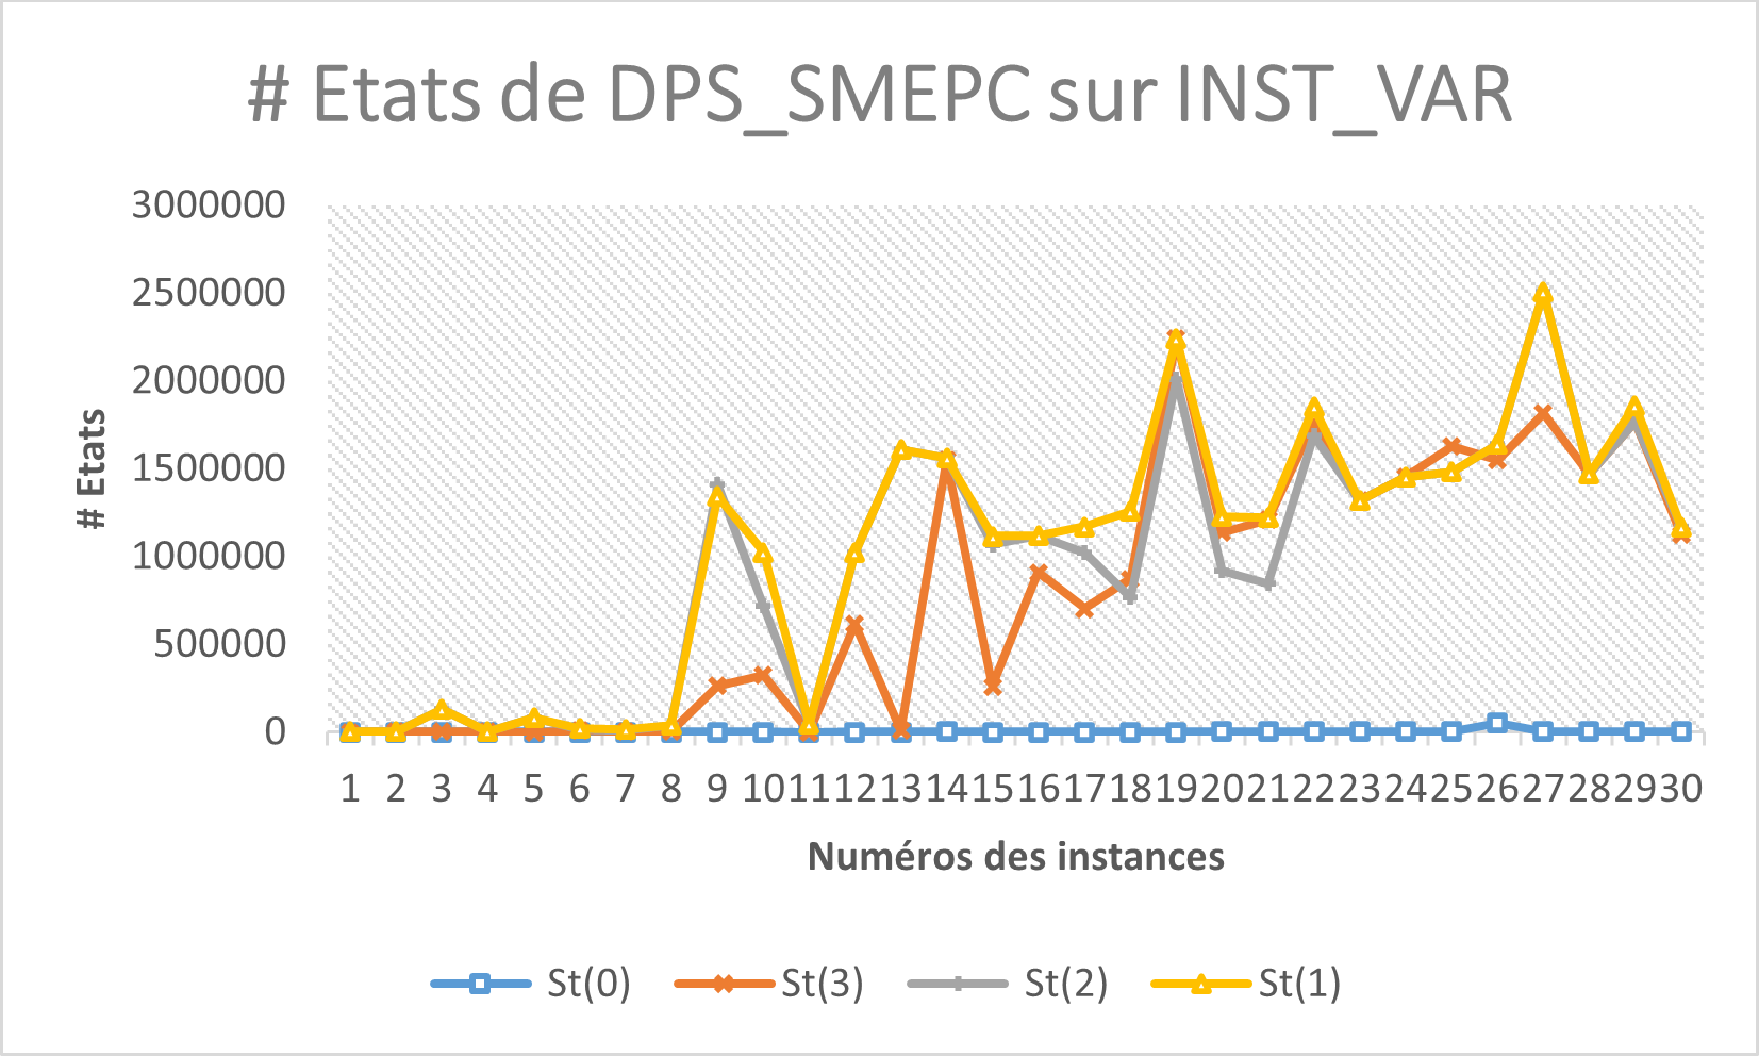
\includegraphics[width=\textwidth]{figures/Etats_DPS_SMEPC_INST_VAR.pdf}
   % \end{column}
  %\end{columns}

  %\begin{columns}[onlytextwidth]
   % \begin{column}{0.5\textwidth}
    %  \centering
    %  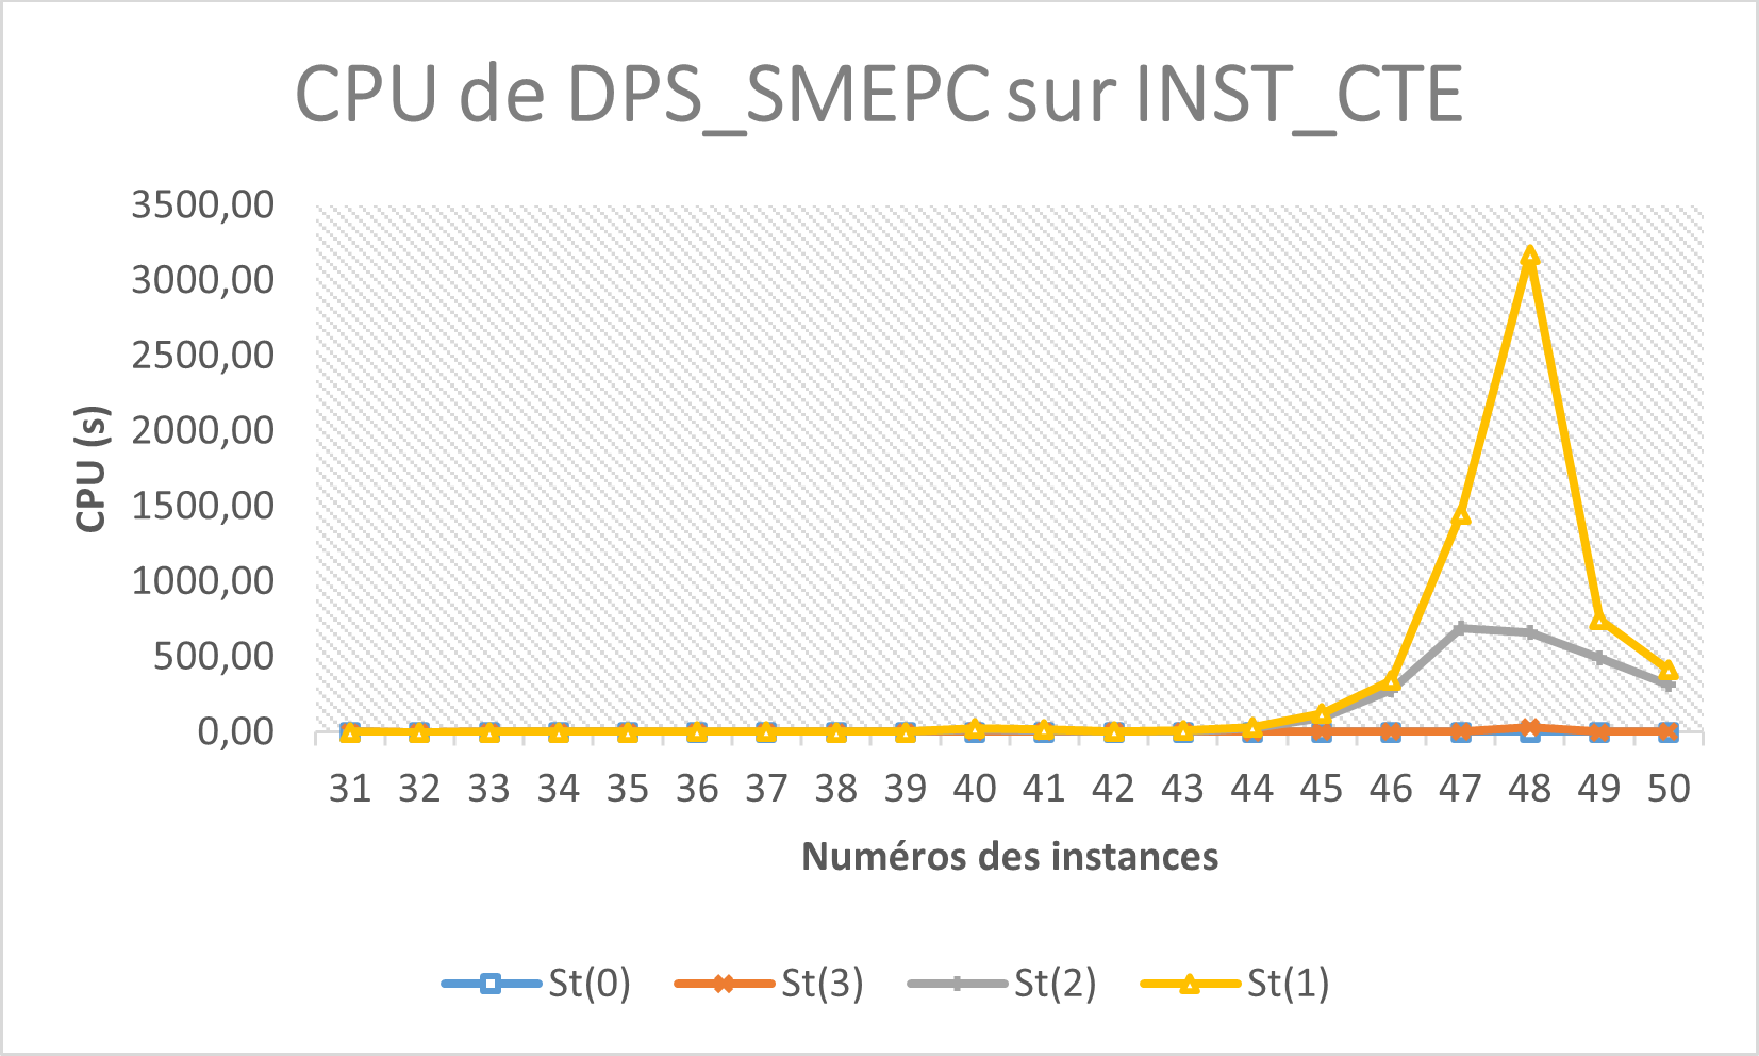
\includegraphics[width=\textwidth]{figures/CPU_DPS_SMEPC_INST_CTE.pdf}
    %\end{column}
    %\begin{column}{0.5\textwidth}
     % \centering
      %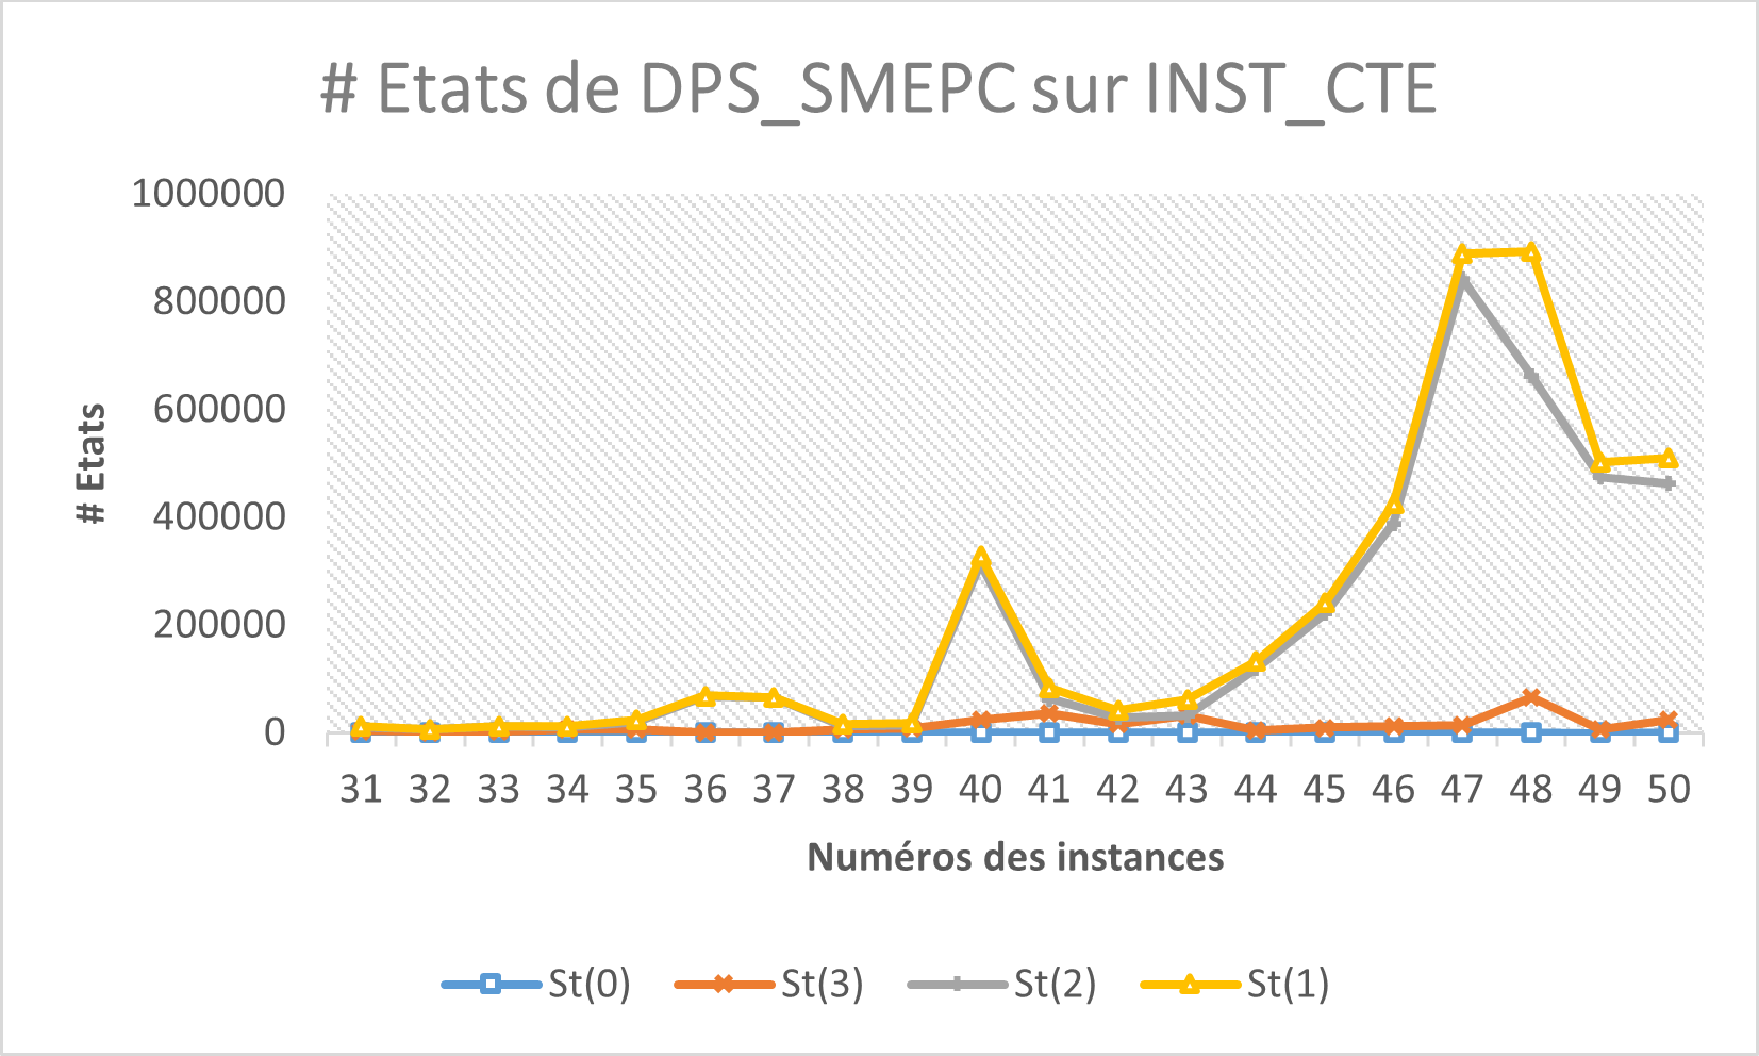
\includegraphics[width=\textwidth]{figures/Etats_DPS_SMEPC_INST_CTE.pdf}
 %   \end{column}
 % \end{columns}
%\end{frame}
%§§§§§§§§§§§§§§§§§§§§§§§§§§§§§§§§§§§§§§§§§§§§§§§§§§§


\begin{frame}
\frametitle{Expérimentations de \textbf{DPS\_SMEPC}}% pour INST\_VAR
\begin{itemize}
%\frametitle{Environnement}
\item Gnu/linux Ubuntu 20.04.2, C++
\item 30 instances
%\item Solution de référence : BSup de MILP (3H)
%\item BSUP : meilleure valeur Greedy-HR, NS(20), NS(50), NS(100)
\end{itemize}

\begin{figure}[H]
	\centering
	\begin{tabular}{c c}
		\includegraphics[width=6.5cm]{figures/sombre_slide_CPU_DPs_SMEPC_INST_VAR.pdf}&%CPU_DPS_SMEPC_INST_VAR
		\includegraphics[width=6.5cm]{figures/sombre_slide_Etats_DPS_SMEPC_INST_VAR.pdf}%Etats_DPS_SMEPC_INST_VAR
		\\
		(a) & (b)
	\end{tabular}
	\caption{(a) représente le temps CPU et (b) représente le nombre d'états engendrés par chaque règle de filtrage.}\label{gap_cpu_DPS_SMEPC_INST_VAR}% de INST\_VAR
\end{figure}
\end{frame}

%\begin{frame}
%\frametitle{\textbf{DPS\_SMEPC} pour %INST\_CTE}
%\begin{figure}[H]
%	\centering
%	\begin{tabular}{c c}
%		\includegraphics[width=6.5cm]{figures/CPU_DPS_SMEPC_INST_CTE.pdf}&
%		\includegraphics[width=6.5cm]{figures/Etats_DPS_SMEPC_INST_CTE.pdf}
%		\\
%		(a) & (b)
%	\end{tabular}
%	\caption{(a) représente le temps CPU et (b) représente le nombre d'états de chaque instance de INST\_CTE.}\label{gap_cpu_DPS_SMEPC_INST_CTE}
%\end{figure}
%\end{frame}



%\begin{frame}
%\frametitle{\# Etats Pipe-line VD\_PM pour INST\_VAR et INST\_CTE}
%\begin{figure}[H]
%	\centering
%	\begin{tabular}{c c}
%		\includegraphics[width=6.5cm]{figures/Etat_Pipe_INST_VAR.pdf}&
%		\includegraphics[width=6.5cm]{figures/Etat_Pipe_INST_CTE.pdf}
%		\\
%		(a) & (b)
%	\end{tabular}
%	\caption{(a) représente le nombre d'états de \textbf{Pipe-line VD\_PM} sur INST\_VAR et (b) représente le nombre d'états de \textbf{Pipe-line VD\_PM} sur INST\_CTE.}\label{gap_cpu_pipe_INST_VAR}
%\end{figure}
%\end{frame}


\subsection{Complexité}
\begin{frame}
\frametitle{Plan}
\addtocounter{framenumber}{-1}
\tableofcontents[currentsection,currentsubsection]
\end{frame}


\begin{frame}
\frametitle{Complexité}



 \begin{block}{Résultats de complexité de SMEPC à Tour Fixé}
SMEPC à tour fixé est Pseudo-Polynomial (polynomial si on
impose des bornes sur les quantités coûts, rendement de production, niveaux de consommation et temps de
parcours, etc.).
 \end{block}
 \end{frame}
 

\section{Résolution heuristique}

%\subsection{Motivations}
%\begin{frame}
%\frametitle{Motivations}
%\begin{itemize}
%\item Temps d'éxécution élevé pour les instances de grandes tailles
%\end{itemize}
%\end{frame}

%\subsection{Heuristique \textbf{\textit{Greedy-SMEPC(NS)}}}

%\begin{frame}
%\frametitle{Heuristique \textbf{\textit{Greedy-SMEPC(NS)}}}
%\begin{itemize}
%\end{itemize}
%\end{frame}
\subsection{DPS filtré par \textit{rounding} et par nombre d’états}
\begin{frame}
\frametitle{DPS Filtré par \textit{Rounding} et par Nombre d’Etats}
\begin{enumerate}
\item \textbf{DPS + Rounding} : Programmation Dynamique \textbf{Filtrée par \textit{Rounding}} : DPS SMEPC auquel on ajoute le filtrage heuristique (\textit{rounding} : conservation d'un unique état par classe d’équivalence ou états modulo K); 
%\vspace{3}

Les états sont équivalents modulo K si :
\begin{itemize}
\item les K premiers bits de la représentation binaire en base 2 de ces états sont identiques.
\item l'écart entre ces états est inférieur à une valeur dépendant de K.
\end{itemize}
%\pause
%\begin{table}[H]
%	\centering
%	\begin{tabular}{|c||c||c||c|}
%		\hline
%		Temps & Etat & Coût & Décision\\ 
%		\hline
%		$(i_0,j_0)$ & $E_0$&$W_0$ & $D$ \\ 
%		\hline
%		$(i,j)$ &  $E=(Z, T, V^{Tank}, V^{Veh})$& $W$ & \dots \\ 
%		\hline
%	\end{tabular}
%\end{table}
%\vspace{3}

% $\forall$ $ E_1=(Z_1, T_1, V^{Tank}_1, V^{Veh}_1)$ appartenant au temps $(i,j)$ et accompagné d'une valeur $W_1$ :
 %	\begin{itemize}
 %	\item Si $Z =Z_1$
  %      \item et $|V^{Tank} - V^{Tank}_1| \leq (C^{Tank} / K)$ 
   %     \item et $|V^{Veh} - V^{Veh}_1| \leq (C^{Veh} / K)$ 
    %    \item et $|T - T_1| \leq ((TMax - \sum_{ j \leq s \leq M}d_s -\sum_{ 0 \leq s \leq j-1} d_s) / K)$ alors on dit que $E$ et $E_1$ sont équivalents modulo $K$ :
 	%\begin{itemize}
 	%	\item si $W<W_1$ alors on remplace $E_1$ par $E$ ;
 	%	\item sinon on n'insère pas $E$ au temps $(i,j)$;
 	%\end{itemize}
%\end{itemize}
\pause
\item \textbf{ Greedy-SMEPC}(NS) - Programmation Dynamique \textbf{Filtrée par Nombre d’Etats} : Sélection des NS meilleurs états à chaque pas de temps DPS.
\end{enumerate}
\end{frame}



\subsection{Heuristique \textbf{\textit{Pipe-Line}}}
\begin{frame}
\frametitle{Plan}
\addtocounter{framenumber}{-1}
\tableofcontents[currentsection,currentsubsection]
\end{frame}

\begin{frame}
	\frametitle{Heuristique Pipe-Line (1/2) }
\begin{figure}
    \centering
   \includegraphics[width=390]{./figures/slide_Pipeline.pdf}
    %\caption{Structure de Pipe-Line.}
    \label{fig:my_label}
\end{figure}
 
\begin {enumerate}
%\item Fixer les paramètres des fonctions de coût. 
\item Résoudre, via le \textcolor{red}{DPS Vehicule}, l'instance du véhicule calculée pour obtenir le nombre de recharges $Q$ ainsi que les vecteurs $m$, $M$ et $\mu$. 
%\item Calculer la borne supérieure d'une solution initiale de l'instance de production résultante via le \textcolor{green}{DPS Greedy-Production}. 
\item Résoudre l'instance de production à travers le \textcolor{blue}{DPS Production}. 
%\item Reconstituer l'ensemble de la solution du problème du SMEPC (à la fois la visite du véhicule et l'activité de la micro-usine), ainsi que sa valeur.
 \end {enumerate}
%\textbf{Pi(1)} $\simeq$ \textbf{ST(1)},  \textbf{Pi(2)} $\simeq$ \textbf{ST(2)},  \textbf{Pi(3)}$\simeq$ \textbf{ST(3)},  \textbf{Pi(0)} $\simeq$ \textbf{ST(0)} 

%\begin{itemize}
	    
%\item  l'INSTANT au sens programmation dynamique est (i) : i = station (0...Nombre de stations+1 )

%\item les ETATS, associes a un instant (i) sont (V,T, pere) :
%\begin{itemize}
%\item 		V = energie dans le vehicule en i
%\item 		T = date de passage du vehicule en i
%\item pere est decrit par un entier qui permet de retrouver l'etat pere dans le tableaux des etats
%\end{itemize}
%\item les DECISIONS x pour l'instant i et un etat (V,T, pere) sont :
%\begin{itemize}
%\item x = 0 le vehicule se deplace de la sation i a la station i+1
%\item  x = 1 le vehicule se recharger entre la station i et la station i+1
%\end{itemize}
%\item Valeur :
%	\end{itemize}
	\end{frame}
\begin{frame}
	\frametitle{Heuristique Pipe-Line (2/2)}
\begin{enumerate}

\item<1-> \textcolor{red}{DPS Vehicule} : DPS\_VD

\begin{itemize}
\item Temps DPS : Temps station ($j$)
\item Etats %($[j-1,j]$)
\begin{itemize}
%\item Station $i$ sur laquelle le véhicule se trouve
\item Date d'arrivée du véhicule en j ($T$) ;
\item Réservoir du véhicule ($V^{Veh}$).
\end{itemize}
\item Décisions %($[j,j+1]$)
\begin{itemize}
\item Décision de recharger($x$)
\end{itemize}

%\item $\sum_{t=0 \dots N-1} (C_f.q_t+C_t .z_t) + \lambda.T_{n+1}$
\item Etat initial : (0,$E_0$), Etats finaux : $(T\leq TMax, V^{Veh}\leq E_0)$ %(\textit{Backward})
 
\end{itemize}



\item<2-> \textcolor{blue}{DPS Production} : DPS\_PM

\begin{itemize}
\item Temps DPS : Temps usine ($i$)
\item Etats %($[i-1,i]$)
\begin{itemize}
%\item Station $i$ sur laquelle le véhicule se trouve
\item \'{E}tat de la micro-usine ($Z$) ;
\item Citerne ($V^{Tank}$) ;
\item Numéro de la dernière opération de recharge effectuée ($Rank \in {1, \dots, Q}$
) ;
\item  Différence entre i et la période de la $Rank^{ième}$ recharge effectuée ($Gap$).
\end{itemize}
\item Décisions %($[i,i+1]$)
\begin{itemize}
\item Décision de produire (z) ;
\item Choix période de recharge ($\delta$).
\end{itemize}
\item Etat initial : (0,$H_0$,0,0), Etats finaux : $(Z, V^{Tank}\geq H_0, Q,0)$ %(\textit{Forward})

\end{itemize}

\end{enumerate}
\end{frame}


%	\begin{frame}
%	\frametitle{Pipe-Line(2/3) : problème production }

%\begin{itemize}


%\item l'INSTANT au sens programmation dynamique est (t) : t = station (0 ...Nombre de p periode)

%\item les ETATS, associes a un instant (t) sont (Z, VTank, Rank, Gap, pere) : 
%\begin{itemize}
%\item		$Z_t$ = Etat de la machine de production d'hydrogene au debut de la periode t
%\item	 $V^Tank$ = stock d'hydrogene dans la citerne au debut de la periode t
%\item		$ Rang \in 1..S$ = l'opération de ravitaillement en carburant portant le numéro Rang a ete effectuee et que nous attendons pour effectuer la prochaine operation de ravitaillement en carburant portant le numero Rang + 1.  
%\item Gap = l'ecart entre t et la periode a laquelle la Rang ieme recharge  a ete effectuee. 
%\itempere est decrit par un entier qui permet de retrouver l'etat pere dans le tableaux des etats
%\end{itemize}
%\item les DECISIONS (z,delta) pour l'instant t et un etat (Z, VTank, Rank, Gap, pere) sont :
%\begin{itemize}
%\item	z = 1 si l'usine produit de l'hydrogene a la periode [t,t+1]
%\item	delta = 1 si le vehicule se recharge en hydrogene a la periode [t,t+1] 
%\end{itemize}
%\item Valeur :
%	\end{itemize}

%\end{frame}
%\begin{frame}
%	\frametitle{Pipe-Line(2/2) }
%	Input: We suppose that we are provided with all data related to the micro-plant and the vehicle, as well as with the coefficient ;
%Output: Production vector z = (zi, i = 0..N-1), activation vector y = (yi, i = 0..N-1), micro-plant refueling vector  = (i, i = 0..N-1),  vehicle refueling vector x = (xj, j = 0,.., M), time vector T = (Tj, j = 0,.., M+1) load vector L = (Lj, j = 0..M), which tells us, in case xj = 1, which H2 quantity is involved, and value VAL =  i = 0..N -1 (CostF.yi + CostVi..zi) + .TM+1 .

 

%\end{frame}
%\section{Expérimentations}
%\begin{frame}
%\frametitle{Expérimentations}
%\begin{figure}
%\begin{minipage}[t]{.4\linewidth}
 %   \begin{center}
 %      \includegraphics[scale=0.5]{./figures/temps_BSUP.pdf}
%     \caption{Coût BSUP}
 %      \label{nbabo}
 %   \end{center}
%\end{minipage}
%\hfill
%\begin{minipage}[t]{.4\linewidth}
%    \begin{center}
%       \includegraphics[scale=0.5]{./figures/cout_BSUP.pdf}
%       \caption{Temps BSUP}
%       \label{croissnbabo}
%    \end{center}
%\end{minipage}
%\end{figure}
%\end{frame}

\subsection{Heuristique \textbf{\textit{Greedy-HR}}}%Heuristique \textbf{\textit{He}}
\begin{frame}
\frametitle{Plan}
\addtocounter{framenumber}{-1}
\tableofcontents[currentsection,currentsubsection]
\end{frame}
\begin{frame}
\frametitle{Heuristique \textbf{\textit{Greedy-HR}}}
\begin{enumerate}
\item<1-> \textbf{Idée} : Conception d'une Heuristique Rapide (HR) avec le problème de production résolu par approche gloutonne.
\item<2-> Le problème du véhicule peut être modélisé en un problème de plus court chemin dans un graphe $G$ :
\begin{itemize}
	\item \textbf{Arcs de type} 1 : arc $(j,j' )$ si $MU$,$j+1$ $\dots$ $j'$,$MU$ réalisable sans recharge %indique que le véhicule est capable de se rendre de la micro-usine (après la station $j$) à la micro-usine (après la station $j'$) sans opération de recharge (). 
	\item \textbf{Arcs de type} 2 : Un arc $(0,j)$ si
	 ($0$, $MU$) réalisable sans recharge (si $j=0$) %le véhicule peut aller du dépôt à la micro-usine juste après le dépôt ;
		ou  ($0$, $j$) réalisable sans recharge (si $j\geq1$). %le véhicule peut aller du dépôt à la station $j$ sans faire le plein (si $j\geq1$).
	
	\item \textbf{Arcs de type} 3 : arc $(j,M+1) $ si $MU$,$j+1$ $\dots$ $M+1$ réalisable sans recharge.%le véhicule peut aller de la micro-usine après la station $j$, jusqu'au dépôt final sans faire le plein. De plus, le véhicule doit arriver au dépôt avec au moins son énergie initiale $E_0$.
\end{itemize}
\item<3-> Après le calcul de la meilleure stratégie de recharge, on calcule la meilleure stratégie de production par approche gloutonne :
\begin{itemize}
	\item Produire le plus tôt possible ;% l'énergie que le véhicule viendra recharger ;
		\item Trouver la meilleure façon de produire entre deux recharges.%, c'est-à-dire au coût le plus bas pour satisfaire la recharge. 
	\end{itemize}
 \end{enumerate}
\end{frame}


%\begin{frame}
%  \frametitle{\textbf{He} et \textbf{Greedy-SMEPC}(NS) pour INST\_VAR et INST\_CTE}

%  \begin{columns}[onlytextwidth]
%    \begin{column}{0.5\textwidth}
%      \centering
%      \includegraphics[width=\textwidth]{figures/CPU_NS_INST_VAR.pdf}
%    \end{column}
%    \begin{column}{0.5\textwidth}
%      \centering
%      \includegraphics[width=\textwidth]{figures/Gap_NS_INST_VAR.pdf}
%    \end{column}
%  \end{columns}

%  \begin{columns}[onlytextwidth]
%    \begin{column}{0.5\textwidth}
 %     \centering
 %     \includegraphics[width=\textwidth]{figures/CPU_NS_INST_CTE.pdf}
 %   \end{column}
  %  \begin{column}{0.5\textwidth}
   %   \centering
 %     \includegraphics[width=\textwidth]{figures/Gap_NS_INST_CTE.pdf}
%    \end{column}
%  \end{columns}
%\end{frame}
%§§§§§§§§§§§§§§§§§§§§§§§§§§§§§§§§§§§§§§§§§§§§§§§§§§§


\begin{frame}
\frametitle{Expérimentations des Heuristiques}% pour INST\_VAR
\begin{itemize}
\item Gnu/linux Ubuntu 20.04.2, C++
\item 30 instances
\item Solution de référence : \textbf{BSup} de MILP (3H), $Gap=100 \times \frac{\textbf{BSup}-Val}{\textbf{BSup}}$
%\item BSUP : meilleure valeur Greedy-HR, NS(20), NS(50), NS(100)
\end{itemize}

\begin{figure}[H]
	\centering
	%\begin{tabular}{c c}
		\includegraphics[width=10.5cm]{figures/slide_Gap_Heuristiques_INST_VAR.pdf}&%CPU_NS_INST_VAR
		%\includegraphics[width=6.5cm]{figures/Gap_NS_INST_VAR.pdf}
		%\\
		%(a) & (b)
	%\end{tabular}
	%\caption{(a) représente le temps CPU et (b) représente le gap pour chaque instance.}\label{gap_cpu_NS_INST_VAR}% de INST\_VAR
\end{figure}
\end{frame}

\begin{frame}
\frametitle{Expérimentations des Heuristiques}% pour INST\_VAR
\addtocounter{framenumber}{-1}
\begin{itemize}
\item Gnu/linux Ubuntu 20.04.2, C++
\item 30 instances
\item Solution de référence : \textbf{BSup} de MILP (3H), $Gap=100 \times \frac{\textbf{BSup}-Val}{\textbf{BSup}}$
%\item BSUP : meilleure valeur Greedy-HR, NS(20), NS(50), NS(100)
\end{itemize}
\begin{figure}[H]
	\centering
	%\begin{tabular}{c c}
		\includegraphics[width=11.5cm]{figures/separateur_slide_Gap_Heuristiques_INST_VAR.pdf}&%CPU_NS_INST_VAR
		%\includegraphics[width=6.5cm]{figures/Gap_NS_INST_VAR.pdf}
		%\\
		%(a) & (b)
	%\end{tabular}
	%\caption{(a) représente le temps CPU et (b) représente le gap pour chaque instance.}\label{gap_cpu_NS_INST_VAR}% de INST\_VAR
\end{figure}
\end{frame}

%\begin{frame}
%\frametitle{ \textbf{He} et \textbf{Greedy-SMEPC}(NS) pour INST\_CTE}
%\begin{figure}[H]
%	\centering
%	\begin{tabular}{c c}
%		\includegraphics[width=6.5cm]{figures/CPU_NS_INST_CTE.pdf}&
%		\includegraphics[width=6.5cm]{figures/Gap_NS_INST_CTE.pdf}
%		\\
%		(a) & (b)
%	\end{tabular}
%	\caption{(a) représente le temps CPU et (b) représente le gap pour chaque instance de INST\_CTE.}\label{gap_cpu_NS_INST_CTE}
%\end{figure}
%\end{frame}

%\begin{frame}
 % \frametitle{Pipe-line VD\_PM pour INST\_VAR et INST\_CTE}

%  \begin{columns}[onlytextwidth]
%    \begin{column}{0.5\textwidth}
%      \centering
%      \includegraphics[width=\textwidth]{figures/CPU_Pipe_INST_VAR.pdf}
%    \end{column}
%    \begin{column}{0.5\textwidth}
%      \centering
%      \includegraphics[width=\textwidth]{figures/Gap_Pipe_INST_VAR.pdf}
%    \end{column}
%  \end{columns}

%  \begin{columns}[onlytextwidth]
%    \begin{column}{0.5\textwidth}
%      \centering
%      \includegraphics[width=\textwidth]{figures/CPU_Pipe_INST_CTE.pdf}
%    \end{column}
%    \begin{column}{0.5\textwidth}
%      \centering
%      \includegraphics[width=\textwidth]{figures/Gap_Pipe_INST_CTE.pdf}
%    \end{column}
%  \end{columns}
%\end{frame}
%§§§§§§§§§§§§§§§§§§§§§§§§§§§§§§§§§§§§§§§§§§§§§§§§§§§

%%\begin{frame}
%%\frametitle{Expérimentations des Heuristiques }%pour INST\_VAR
%\begin{itemize}
%\item Gnu/linux Ubuntu 20.04.2, C++
%\item 30 instances, Solution de référence : BSup de MILP (3H)
%\item BSUP : meilleure valeur Greedy-HR, NS(20), NS(50), NS(100)
%\end{itemize}
%%\begin{figure}[H]
%%	\centering
%%	\begin{tabular}{c c}
%%		\includegraphics[width=6.5cm]{figures/slide_CPU_NS_Heuristiques_INST_VAR.pdf}&%CPU_Pipe_INST_VAR
%%		\includegraphics[width=6.5cm]{figures/slide_CPU_ST_Pi_Heuristiques_INST_VAR.pdf}%Gap_Pipe_INST_VAR
		%\\
		%(a) & (b)
%%	\end{tabular}
	%\caption{Temps CPU des heuristiques}\label{gap_cpu_pipe_INST_VAR}% de INST\_VAR
 %(a) représente le temps CPU et (b) représente le gap de chaque instance.
%%\end{figure}
%%\end{frame}

%\begin{frame}
%\frametitle{Pipe-line VD\_PM pour INST\_CTE}
%\begin{figure}[H]
%	\centering
%	\begin{tabular}{c c}
%		\includegraphics[width=6.5cm]{figures/CPU_Pipe_INST_CTE.pdf}&
%		\includegraphics[width=6.5cm]{figures/Gap_Pipe_INST_CTE.pdf}
%		\\
%		(a) & (b)
%	\end{tabular}
%	\caption{(a) représente le temps CPU et (b) représente le gap de chaque instance de INST\_CTE.}\label{gap_cpu_pipe_INST_VAR}
%\end{figure}
%\end{frame}


\section{Problème à Tour Libre}% : réseau de neurones artificiels
%\subsection{Apprentissage supervisé : réseau de neurones artificiels}
%\begin{frame}
%\frametitle{Réseau de neurones SIMPLE\_PERIODE et SIMPLE\_TYPE}

%\begin{figure}[H]
%	\centering
%		\includegraphics[width=11cm]{figures/SFC2.pdf}
	%\caption{Ceci représente SIMPLE\_PERIODE.}
%\end{figure}

%Pour le réseau SIMPLE\_TYPE, les données sont regroupées par type.

%\end{frame}
\subsection{Motivation}
\begin{frame}
\frametitle{Schéma d’Elimination de la Production}

\begin{enumerate}
\item<+-> \textbf{Idée} 

Le tour augmenté de ses détours \enquote{recharges} (tour plein $\Gamma$) devient la variable
principale : On élimine toute la partie \enquote{Production} et on la remplace par un estimateur
\enquote{Surrogate} Surr qui sépare les bons tours des mauvais.

\item<+-> \textbf{Schéma algorithmique} 

Il s’appuie sur cet estimateur devient un schéma classique
d’amélioration locale, mettant en jeu un opérateur Trans($\Gamma$, $\lambda$) :
\begin{itemize}
\item Initialiser $\Gamma$ ; Not Stop ;
\item Tant que Not Stop faire
\begin{itemize}
\item Chercher $\lambda$ tel que appliquer Trans($\Gamma$, $\lambda$) améliore Surr($\Gamma$) ;
\item Si Echec(Chercher) alors Stop ;
\end{itemize}
\end{itemize}
\item<+-> \textbf{Question : Quel opérateur Surr ? }

\begin{alertblock}<+->{Notre approche}
Surr est la sortie d’un réseau de neurones qui estime le coût SMEPC induit par $\Gamma$ :
\begin{enumerate}
\item MIXTE\_*
\item INDIC\_*
\end{enumerate}
 \end{alertblock}


%\begin{itemize}
%\item Ajout de la planification de la tournée 
%\item Besoin d'évaluation rapide de la qualité d'une tournée
%\item Construction d'un estimateur du coût d'une tournée
%\end{itemize}
\end{enumerate}
\end{frame}
\subsection{Réseaux de neurones}% \textbf{\textit{MIXTE\_*}} et \textbf{\textit{INDIC\_*}}
\begin{frame}
\frametitle{Réseau de neurones MIXTE\_TEMPS et MIXTE\_COUT}
\begin{figure}[H]
	\centering
		\includegraphics[width=9.8cm]{figures/slide_FNFC.pdf}
%\caption{Ceci représente MIXTE\_TEMPS et MIXTE\_COUT.}
\end{figure}
\end{frame}
\begin{frame}

%\subsection{Réseau de neurones INDIC\_TEMPS  et INDIC\_COUT}
\frametitle{Réseau de neurones INDIC\_TEMPS }
\begin{itemize}
\item Indicateur $a_0=H_0/\sum \mu$ : plus sa valeur augmente, plus la valeur de T diminue. On a moins de données et de couches.
%\item	$T = Ga \times (m_Q + De) + (1 - Ga) \times M_Q$ avec $Ga \in  [0, 1]$ ;
%\item	$Ga = \Phi^x(X)$, où $\Phi^x$ = $Exp(x.X)/(Exp(x.X)+1)$, $x \geq 0$; $X = w_0.(H_0/Mu)$ $+w_1.(P^*/N) +  w_2.(A^*/N)+  w_3.C +  w_4.C^* - w_5.K$ $  - w_6.I^0/N $ $- w_7$%,  où $w_0, w_1, \dots, w_6 \geq 0$ et $w_7$ est non signé.
\end{itemize}
\begin{figure}[H]
	\centering
		\includegraphics[width=9.7cm]{figures/slide_time_value_scheme.pdf}
%\caption{Ceci représente MIXTE\_TEMPS et MIXTE\_COUT.}
\end{figure}


\end{frame}

%\begin{figure}
% \begin{center}
%       \includegraphics[scale=0.046]{figures/im_1_PROD_cost_value.pdf}
%     \caption{Problème de production.}
%       \label{NS_GAP}
%\end{center}
%\end{figure}

%\end{frame}
\begin{comment}

\begin{frame}
\frametitle{Expérimentations (1/6) : instances}
\begin{table}[htbp]
\begin{center}
\begin{tabular}{|*{6}{c|}}
\hline
Instance & M&N&p&Cost^F&Mean\_Cost^V\\ \hline
1&4&15&4&1&1,0\\\hline
2&8&25&4&21&1,1\\\hline
3&8&26&4&12&4,1\\\hline
4&8&26&4&15&2,8\\\hline
5&8&27&4&22&2,1\\\hline
6&8&30&4&22&3,5\\\hline
7&10&17&4&9&5,4\\\hline
8&10&19&4&9&2,1\\\hline
9&10&20&4&8&2,3\\\hline
10&10&36&2&25&4,6\\\hline
11&10&50&4&7&3,3\\\hline
12&10&57&2&13&1,9\\\hline
13&10&78&1&3&4,2\\\hline
14&12&32&4&31&4,7\\\hline
\end{tabular}
\caption{Instances : 14 instances, C++, Visual Studio 2017,  16 Go de RAM, CPLEX 12.8. \label{instances}}
\end{center}
\end{table}
\end{frame}

\begin{frame}
\frametitle{Expérimentations (2/6) : MIP et modèle fractionnaire}
\begin{table}[htbp]
\begin{center}
\begin{tabular}{|*{7}{c|}}
\hline
Inst.& PL\_G(\%)& PL\_T(s) & FRAC\_G(\%)& FRAC\_T(s)& F\_G(\%)& F\_T(s)\\\hline
1&0&0,1&100&0,013&-19,2&0,024\\\hline
2&0&0,6&100&0,025&-45,9&0,043\\\hline
3&0&0,7&100&0,029&-53,3&0,053\\\hline
4&0&0,3&100&0,023&-32,1&0,038\\\hline
5&0&0,4&100&0,023&-45,8&0,052\\\hline
6&0&0,7&100&0,026&-35,2&0,051\\\hline
7&0&0,2&100&0,021&-31,3&0,033\\\hline
8&0&0,1&100&0,02&-31,2&0,063\\\hline
9&0&0,3&100&0,022&-35,4&0,038\\\hline
10&0&0,3&100&0,034&-29,8&0,069\\\hline
11&0&1,6&100&0,045&-36,7&0,093\\\hline
12&0&1,3&100&0,083&-18,5&0,12\\\hline
13&0&0,6&100&0,098&-11,0&0,174\\\hline
14&0&2,3&100&0,034&-26,9&0,097\\\hline
%1&0&&100&&&\\\hline
%2&0&&100&&&\\\hline
%3&0&&100&&&\\\hline
%4&0&&100&&&\\\hline
%5&0&&100&&&\\\hline
%6&0&&100&&&\\\hline
%7&0&&100&&&\\\hline
%8&0&&100&&&\\\hline
%9&0&&100&&&\\\hline
%10&0&&100&&&\\\hline
%11&0&&100&&&\\\hline
%12&0&&100&&&\\\hline
%13&0&&100&&&\\\hline
%14&0&&100&&&\\\hline

\end{tabular}
\caption{Valeurs PL\_G, PL\_T, FRAC\_G, FRAC\_T, F\_G, F\_T. \label{PL_FRAC}}
\end{center}
\end{table}
\end{frame}

%\begin{frame}
%\frametitle{Expérimentations (3/6) : DPS-SMEPC et NS}

%\begin{table}[htbp]
%\begin{center}
%\begin{tabular}{|*{5}{c|}}
%\hline
%Inst.& G\_G(\%)& G\_T(s)& W\_G(20)(\%)& W\_T(20)(s) \\\hline
%1&2,2&0,1&2,2&0,1\\\hline
%2&33&0,3&31,5&0,4\\\hline
%3&5,2&0,4&    5,2&0,4\\\hline
%4&31,2&0,2&30,5&0,3\\\hline
%5&0&0,1&0&0,1\\\hline
%6&12,1&0,3&12,1&0,3\\\hline
%7&23,1&0,2&10,8&0,3\\\hline
%8&19,6&0,1&19,6&0,2\\\hline
%9&2,5&0,2&0,8&0,2\\\hline
%10&44,3&0,3&42,3&0,4\\\hline
%11&6,9&0,4&6,9&0,6\\\hline
%12&11,3&0,6&10,6&0,8\\\hline
%13&47,9&0,7&42,6&1,0\\\hline
%14&6,4&0,3&6,4&0,4\\\hline
%\end{tabular}
%\caption{Valeurs G-Gap, W-Gap(x). \label{GAP}}
%\end{center}
%\end{table}

%\end{frame}

\begin{frame}
\frametitle{Expérimentations (3/6) : DPS-SMEPC et NS}
\begin{figure}
\begin{minipage}[t]{.4\linewidth}
    \begin{center}
       \includegraphics[scale=0.45]{./figures/NS_GAP.jpg}
     \caption{Valeurs G-Gap, W-Gap(x).}
       \label{NS_GAP}
\end{center}
\end{minipage}
\hspace{0.55cm}
\begin{minipage}[t]{.4\linewidth}
    \begin{center}
      \includegraphics[scale=0.43]{./figures/NS_TEMPS.jpg}
       
      \caption{Valeurs G-Gap, W-Gap(x).}
       \label{NS_TEMPS}
    \end{center}
\end{minipage}
\end{figure}
%\begin{table}[htbp]
%\begin{center}
%\begin{tabular}{|*{5}{c|}}
%\hline
%Inst.& W\_G(50)(\%)& W\_T(50)(s)& W\_G(100)(\%)& W\_T(100)(s)\\\hline
%1&0&0,1&0&0,2\\\hline
%2&10,2&0,6&0&1,0\\\hline
%3&0&0,7&0&1,2\\\hline
%4&19,9&0,4&0&0,7\\\hline
%5&0&0,1&0&0,2\\\hline
%6&21,6&0,5&0&0,9\\\hline
%7&0&0,5&0&0,8\\\hline
%8&15,9&0,3&0&0,4\\\hline
%9&0,8&0,3&0&0,4\\\hline
%10&37,1&0,6&0&1,1\\\hline
%11&6,9&1,1&6,1&2,0\\\hline
%12&9,2&1,3&6,4&2,2\\\hline
%13&35,1&1,7&9,6&2,8\\\hline
%14&5,7&0,7&2,7&1,2\\\hline
%\end{tabular}
%\caption{Valeurs G-Gap, W-Gap(x). \label{GAP}}
%\end{center}
%\end{table}

\end{frame}

\begin{frame}
\frametitle{Expérimentations (4/6) : Filtrage DPS-SMEPC}
\begin{table}[htbp]
 \begin{center}
\begin{tabular}{|*{8}{c|}}
\hline
Inst.& ST(3)& T(3)(s)& ST(2)& T(2)(s)& ST(1)& T(1)(s)& ST(0)\\\hline
1&28&0,1&421&0,2&487&0,2&576000\\\hline
2&1350&2,1&16658&49,2&16712 &51,7 &705600\\\hline
3&916&1,7&13476&22,0&15011&25,0&718848\\\hline
4&121&0,2&10989&11,5&19183&20,1&2416128\\\hline
5&312&0,2&48501&181,4&48868&186,8&876096\\\hline
6&3014&4,0&13608&27,3&14912&31,6&1614720\\\hline
7&35&0,1&6013&10,0&6572&11,4&199920\\\hline
8&101&0,1&887&0,7& 2284&1,9&291840\\\hline
9&403&0,3&1718&1,1&1927&1,6&291600\\\hline
10&49&0,1&28876&140,5&29760&149,7&1559520\\\hline
11&9675&66,7&118795&1227,7&119347&1233,8&3136000\\\hline
12&1988&11,7&16028&135,7&18323&146,7&1206120\\\hline
13&10329&121,9&31810&492,9&37483&529,8&1137240\\\hline
14&10260&19,1&11589&32,2&15688&42,2&602112\\\hline

\end{tabular}
\caption{Expérimentations des règles de filtrage. \label{table-nom}}
\end{center}
\end{table}
\end{frame}

\begin{frame}
\frametitle{Expérimentations (5/6) : Pipe-Line}
\begin{table}[htbp]
\begin{center}
\begin{tabular}{|*{9}{c|}}
\hline
Inst.&PIPE\_G(\%)&PIPE\_T(s)&ST\_VEH&ST\_PROD\\\hline
1& 2,2 & 0,004 & 1 & 49\\\hline
2 & 0,9 & 0,011 & 13 & 535\\\hline
3 &0& 0,018&10&601\\\hline
4&0& 0,101&5&1159\\\hline
5&1&0,04&19&1909\\\hline
6&0&0,012&1&573\\\hline
7&0&0,01&5&629\\\hline
8&0&0,008&1&174\\\hline
9&2,5&0,008&19&76\\\hline
10&6,2&0,108&1&2900\\\hline
11&1,5&0,164&16&3222\\\hline
12&6,4&0,048&19&1647\\\hline
13&3,2&0,171&15&3024\\\hline
14&2,4&0,011&1&283\\\hline

\end{tabular}
\caption{Valeurs PIPE\_G, PIPE\_T, ST\_VEH, ST\_PROD. \label{PIPEL}}
\end{center}
\end{table}
\end{frame}


\begin{frame}
\begin{itemize}
\frametitle{Environnement}
\item Gnu/linux Ubuntu 20.04.2.
\item C++ , Python
%\item Visual Studio  2017 et 2019 ;
%\item Solveur : CPLEX 12.10 ;
%\item 512 Go de RAM ; 
\item 30 instances %: INST\_VAR 30, INST\_CTE 20 (N=20 pour toutes les instances) ;
%\item Temps : distance Euclidienne, Energie : distance Manhattan ;
\item Recherche d'une borne supérieure : Exécution sucessive de Greedy-HR, NS(20), NS(50), NS(100) en utilisant comme borne supérieure la meilleure déjà obtenue ;
\item Génération aléatoire de 6000 instances pour tester nos réseaux de neurones ;
\item Solution de référence : BSup de MILP (3H) ;%, 8 \textit{threads}
%\item $Gap=100 \times \frac{Opt-Obj}{Opt}$
%\item  $gapMI=100 \times \frac{BSup-BInf}{BSup}$
\end{itemize}
\end{frame}
\end{comment}


\begin{frame}

\begin{itemize}
\item Gnu/linux Ubuntu 20.04.2, Python, Tensorflow/Keras
\item Génération aléatoire de 6000 instances

\end{itemize}
\frametitle{Comparaison de nos réseaux de neurones}
\begin{table}[H]
	\begin{center}
		\begin{tabular}{|c|c|c|c|c|}%{|m{4cm}|m{1.9cm}|m{1.5cm}|m{2cm}|m{1.5cm}|}
			\hline
				Nom du réseau de neurones & \textcolor{blue}{Gap test} (\%)&Gap fit(\%)& \textcolor{red}{\# poids}\\
			\hline
			Réseau \textcolor{blue}{\textbf{MIXTE\_TEMPS}} &11,26 & 8,31& 570 \\
			\hline
			Réseau \textcolor{red}{\textbf{INDIC\_TEMPS}} &13,21 &8,78 &9 \\
			\hline
		\end{tabular}
	\end{center}
	\caption{Apprentissage du numéro de période de la dernière recharge : Moyenne de la valeur absolue des gaps des données de test et d'apprentissage. \label{Gap_time}}
\end{table}

\begin{table}[H]
	\begin{center}
	\begin{tabular}{|c|c|c|c|c|}%{|m{4.5cm}|m{1.9cm}|m{1.5cm}|m{1.5cm}|m{1.5cm}|}
	\hline

	Nom du réseau de neurones & \textcolor{blue}{Gap test} (\%)&Gap fit (\%)& \textcolor{red}{\# poids}\\
	\hline
	%Réseau \textbf{SIMPLE\_TYPE} & 20&25,45&24,8 &697\\
	%\hline
	%Réseau \textbf{SIMPLE\_PERIODE}& 2&23,28 &38,03 & 729\\
	%\hline
	Réseau \textcolor{blue}{\textbf{MIXTE\_COUT}} &17,14 & 14,49&570\\
	\hline
	Réseau \textcolor{red}{\textbf{INDIC\_COUT}} &24,19 &13,27 & 20\\
	\hline
\end{tabular}
	\end{center}
\caption{Apprentissage du coût de production : Moyenne de la valeur absolue des gaps des données de test et d'apprentissage. \label{Gap}}
\end{table}

\end{frame}

\begin{frame}
\frametitle{Réseau de neurones Mixte\_TEMPS}


\begin{figure}[H]
	\centering
	\begin{tabular}{c c}
		\includegraphics[width=6cm]{figures/time_6000_prediction_courbe_Al_He_complet_train.pdf}&
		\includegraphics[width=6cm]{figures/time_6000_prediction_courbe_Al_He_complet_test.pdf}
		\\
		(a) & (b)
	\end{tabular}
	\caption[Résultats du  réseau MIXTE\_TEMPS]{Résultats du  réseau \textbf{MIXTE\_TEMPS} pour la prédiction du numéro de période de la dernière recharge. (a) représente les données d'apprentissage et (b) représente les données de test. Les points rouges sont les valeurs prédites et les points verts sont les valeurs optimales.}\label{time_6000_prediction_courbe_Al_He_complet}
\end{figure}
\end{frame}


\begin{frame}
\frametitle{ Réseau de neurones Mixte\_COUT}

\begin{figure}[H]
	\centering
	\begin{tabular}{c c}
		\includegraphics[width=6cm]{figures/prediction_courbe_Al_He_complet_train.pdf}&
		\includegraphics[width=6cm]{figures/prediction_courbe_Al_He_complet_test.pdf} 
		\\
		(a) & (b)
	\end{tabular}
	\caption[Résultats du  réseau MIXTE\_COUT]{Résultats du  réseau \textbf{MIXTE\_COUT} pour la prédiction du coût de production. (a) représente les données d'apprentissage et (b) représente les données de test. La courbe rouge est la courbe des valeurs prédites et la courbe verte est la courbe des valeurs optimales.}\label{6000_prediction_courbe_Al_He_complet}
\end{figure}
\end{frame}

\section{Conclusion}
%\section{Conclusions et perspectives}

\begin{frame}
\frametitle{Conclusions et perspectives}

\begin{enumerate}
\item<1-> Récapitulatif
\begin{itemize}

\item Présentation d'un nouveau problème ;%qui synchronise tournée de véhicules et production d'hydrogène ;


\item Modèle :
\begin{itemize}
\item MILP : \textit{beaucoup de variables booléennes et entières} ;%, problème difficile à résoudre avec CPLEX à partir de 25 stations.
\space
\item LR : ajout de contraintes additionelles ;
\end{itemize}
\item Algorithme de programmation dynamique : \textit{grand nombre d'états} ;
\item Heuristiques : DPS + Rounding, Greedy-SMEPC(NS), Pipe-Line, Greedy-HR ;
\item Réseaux de neurones pour prédire le coût optimal.
\end{itemize}
\item<2-> Conclusions
\begin{itemize}
%\item MILP a du mal à résoudre des instances de  grandes tailles ;
\item  Filtrage par Rounding : très efficace pour filtrer les états;
\item Filtrage par estimation optimiste : filtrage exacte le plus efficace ;
\item Taille instance \& méthode de résolution.
\end{itemize}
\item<3-> Perpectives
\begin{itemize}
\item \'{E}tendre ces approches à plusieurs véhicules ;
\item Gérer les incertitudes liées à la production d'hydrogène ;
\item Ajouter la planification de la tournée au problème ;
\item Décision collaborative : retour du module esclave vers le module maitre.
\end{itemize}
\end{enumerate}



\end{frame}

%---------------------------------------------------------
%\begin{frame}
%\frametitle{Perpectives}
%\begin{itemize}
%\item Perpectives pour la suite de la thèse
%\begin{enumerate}
%\item Gérer les incertitudes liées à la production d'hydrogène
 %\item Concevoir un procédé de génération d'instances. 
 %\item Finaliser l’approche branch and cut.
%\item Ajouter de la planification de la tournée au problème.
%\item Finaliser la rédaction du rapport de thèse.
%\end{enumerate}
%\vspace{2}
%\item Perpectives du problème
%\begin{enumerate}
%\item Ajouter de la planification de la tournée au problème.
%\item \'{E}tendre ces approches à plusieurs véhicules.
%\item Gérer les incertitudes liées à la production d'hydrogène
%\end{enumerate}
%    \item Variantes du problème du véhicule

 %\begin{itemize}
 %    \item Quantité d'hydrogène chargée à chaque recharge : fixe ou variable (plein du réservoir) ;
  %   \item Durée de la recharge : fixe ou instantanée ;
  %   \item Périodes de recharge interdites.
 %\end{itemize}

 %\item Variantes du problème de production
 %\begin{itemize}
 %    \item Quantité d'hydrogène produite : fixe ou variable ;
 %    \item Périodes de production interdites.
 %\end{itemize}
 

%\end{itemize}
%\end{frame}

\begin{frame}
\frametitle{}

\transboxin % Effet de transition de fondu
\centering{
\begin{Large}
\textbf{Merci de votre attention !} %\\
%\textbf{Questions ?}
\end{Large}
}
%\includegraphics[width=12cm,height=9cm]{./figures/thhhh.jpg}
\end{frame}


%§§§§§§§§§§§§§§§§§§§§§§§§§§§§§§§§§§§§§§§§§§§§§§§§§§§
\begin{frame}
 \addtocounter{framenumber}{-1}
\frametitle{}

\transboxin % Effet de transition de fondu
\centering{
\begin{Large}
\textbf{} %\\
%\textbf{Questions ?}
\end{Large}
}
%\includegraphics[width=12cm,height=9cm]{./figures/thhhh.jpg}
\end{frame}

\begin{frame}
 \addtocounter{framenumber}{-1}
\frametitle{}

\transboxin % Effet de transition de fondu
\centering{
\begin{Large}
\textbf{} %\\
%\textbf{Questions ?}
\end{Large}
}
%\includegraphics[width=12cm,height=9cm]{./figures/thhhh.jpg}
\end{frame}

\begin{frame}
 \addtocounter{framenumber}{-1}
\frametitle{Expérimentations de MILP (1H)}% , \textit{mono-thread}) pour INST\_VAR

\begin{itemize}
%\frametitle{Environnement}
\item Gnu/linux Ubuntu 20.04.2, C++, CPLEX 12.10
\item 30 instances
\end{itemize}
\begin{figure}[H]
	\centering
	\begin{tabular}{c c}
		\includegraphics[width=6.5cm]{figures/slide_CPU_MILP_INST_VAR.pdf}&%CPU_MILP_INST_VAR
		\includegraphics[width=6.5cm]{figures/slide_GAPMI_MILP_INST_VAR.pdf}%gapMI_MILP_INST_VAR
		\\
		(a) & (b)
	\end{tabular}
	\caption{ (a) représente le temps CPU et (b) représente le gap de chaque instance.}\label{gapMI_cpu_RMILP_INST_VAR}% de INST\_VAR.
\end{figure}

\end{frame}

\begin{frame}
\addtocounter{framenumber}{-1}
\frametitle{Expérimentations des Heuristiques }%pour INST\_VAR
%\begin{itemize}
%\item Gnu/linux Ubuntu 20.04.2, C++
%\item 30 instances, Solution de référence : BSup de MILP (3H)
%\item BSUP : meilleure valeur Greedy-HR, NS(20), NS(50), NS(100)
%\end{itemize}
\begin{figure}[H]
	\centering
	\begin{tabular}{c c}
		\includegraphics[width=6.5cm]{figures/slide_CPU_NS_Heuristiques_INST_VAR.pdf}&%CPU_Pipe_INST_VAR
		\includegraphics[width=6.5cm]{figures/slide_CPU_ST_Pi_Heuristiques_INST_VAR.pdf}%Gap_Pipe_INST_VAR
		%\\
		%(a) & (b)
	\end{tabular}
	%\caption{Temps CPU des heuristiques}\label{gap_cpu_pipe_INST_VAR}% de INST\_VAR
 %(a) représente le temps CPU et (b) représente le gap de chaque instance.
\end{figure}
\end{frame}

\begin{frame}
 \addtocounter{framenumber}{-1}
\frametitle{Réseau de neurones INDIC\_COUT (1/2) }
\begin{itemize}
	\item $COST = K.Cost_A + Mu.Cost_P$ 
 \item On a moins de données et de couches.
\end{itemize}
%\begin{itemize}
%\item $Cost_A = (1 + Ta).A$
%(Be(A - A^0) + (1 - Be).(A + A^0))$ avec $Ta \geq 0$ et $Be \in [0, 1]$; 
%\begin{itemize}
%	\item	$Ta = (1/A).(Ta_1.P + Ta_2.P^0 + Ta_3.G-Ta_4.C)$, avec $Ta_1, Ta_2, Ta_3, Ta_4 \geq 0$ ;
	
%\item	$Ta = (R/A).(Ta_1.P + Ta_2.P^0 + Ta_3.G)$, avec $Ta_1, Ta_2, Ta_3 \geq 0$ ;
%\item	$Be = \Phi^y(Y)$ ;
%\item	$Y = Be_1.(A/P.R) + Be_2.(A^*/N) - Be_0$, avec $Be_1, Be_2 \geq 0$ ;
%\end{itemize}
%\item	$Cost_P = \alpha_1.(P - P^0) + \alpha_2.(P + P^0)$ avec $\alpha_1, \alpha_2 \in [0, 1]$; 
%\begin{itemize}
%\item	$\alpha_1 = \Phi^{z1}(Z_1)$ ;
%\item	$Z_1 = -\beta_1.(P^*/N) -  \gamma_1.(P^0/P) + \lambda_1.(A/PR) -  \sigma_1.(V^0/V) -\pi_1.C +\tau_1. (S/N)+ \delta_1$ , où $\beta_1, \gamma_1, \lambda_1, \sigma_1, \pi_1, \tau_1 \geq 0$ et $\delta_1$ est non signé.
%\item	$\alpha_2 = \Phi^{z2}(Z_2)$ ;
%\item	$Z_2 = -\beta_2.(P^*/N) -  \gamma_2.(P^0/P) + \lambda_2.(A/PR) -  \sigma_2.(V^0/V) -\pi_2.C +\tau_2. (S/N)+ \delta_2$ , où $\beta_2, \gamma_2, \lambda_2, \sigma_2, \pi_2, \tau_2 \geq 0$ et $\delta_2$ est non signé.

%\end{itemize}
%\end{itemize}
%Cost_A représente l'estimation du cout d'une activation de la micro-usine
%Cost_P est une valeur entre 0 et 2P qui représente l'estimation du cout de production d'une unité d'hydrogène à recharger


%\begin{figure}[H]
%	\centering
%		\includegraphics[width=6.5cm]{figures/im_1_PROD_cost_value.pdf}&
%		\includegraphics[width=7cm]{figures/im_2_PROD_cost_value.pdf}
%\end{figure}

%\begin{figure}[H]
%	\centering
%	\begin{tabular}{c c}
%		\includegraphics[width=5.4cm]{figures/im_1_PROD_cost_value.pdf}&
%		\includegraphics[width=9cm]{figures/im_2_PROD_cost_value.pdf}
%		\\
%		(a) & (b)
%	\end{tabular}
%	\caption{????}
%\end{figure}
\begin{figure}[H]
	\centering
		%\includegraphics[width=10cm]{figures/im_1_PROD_cost_value.pdf}&
		\includegraphics[width=13.5cm]{figures/slide_im_2_PROD_cost_value.pdf}
\end{figure}
%im_1_PROD_cost_value
%im_2_PROD_cost_value

\end{frame}

\begin{frame}
 \addtocounter{framenumber}{-1}
\frametitle{Réseau de neurones INDIC\_COUT (2/2) }
\begin{figure}[H]
	\centering
		\includegraphics[width=10cm]{figures/slide_im_1_PROD_cost_value.pdf}&
		%\includegraphics[width=7cm]{figures/im_2_PROD_cost_value.pdf}
\end{figure}

\end{frame}


\end{document}